% !Mode:: "TeX:UTF-8"
%# -*- coding:utf-8 -*-

\documentclass[winfonts,master,twoside]{njuthesis}

\usepackage{threeparttable}
% \usepackage{makecell}

\newcommand{\xform}[1]{\texttt{@XForm/#1}}

\renewcommand{\lstlistingname}{代码}

\definecolor{light-gray}{rgb}{0.95, 0.95, 0.95}
\definecolor{darkgray}{rgb}{0.4, 0.4, 0.4}
\definecolor{editor-gray}{rgb}{0.95, 0.95, 0.95}
\definecolor{editor-ocher}{rgb}{1, 0.5, 0} % #FF7F00 -> rgb(239, 169, 0)
\definecolor{editor-green}{rgb}{0, 0.5, 0} % #007C00 -> rgb(0, 124, 0)
\definecolor{orange}{rgb}{1,0.45,0.13}
\definecolor{olive}{rgb}{0.17,0.59,0.20}
\definecolor{brown}{rgb}{0.69,0.31,0.31}
\definecolor{purple}{rgb}{0.38,0.18,0.81}
\definecolor{light-blue}{rgb}{0.1,0.57,0.7}
\definecolor{light-red}{rgb}{1,0.4,0.5}

% JavaScript
\lstdefinelanguage{JavaScript}{
  morekeywords=[3]{typeof, new, true, false, catch, function, return, null, catch, switch, var, if, in, while, do, else, case, break, const},
  keywordstyle=[3]\color{red},
  morecomment=[s]{/*}{*/},
  morecomment=[l]//,
  morestring=[b]",
  morestring=[b]'
}

\lstdefinelanguage{HTML5}{
  language=html,
  sensitive=true,
  alsoletter={<>=-},
  morecomment=[s]{<!--}{-->},
  tag=[s],
  otherkeywords={
      html, body, button, div, script, span, input, Card, Input
    },
  ndkeywords={
      =, charset=, src=, id=, width=, height=, style=, type=, rel=, href=,
    },
  identifierstyle=\color{black},
  keywordstyle=\color{light-blue}\bfseries,
  ndkeywordstyle=\color{editor-green}\bfseries,
  stringstyle=\color{editor-ocher}\ttfamily,
  commentstyle=\color{brown}\ttfamily,
}

\lstdefinestyle{HTML-with-JavaScript} {
  basicstyle={\footnotesize\ttfamily},
  frame=b,
  xleftmargin={0.75cm},
  numbers=left,
  stepnumber=1,
  firstnumber=1,
  numberfirstline=true,
  language=HTML5,
  morekeywords=[3]{function, return},
  keywordstyle=[3]\color{light-red},
  morekeywords=[4]{const},
  keywordstyle=[4]\color{red},
  morecomment=[s]{/*}{*/},
  morecomment=[l]//,
  alsodigit={.:;},
  tabsize=2,
  showtabs=false,
  showspaces=false,
  showstringspaces=false,
  extendedchars=true,
  breaklines=true
}

\lstdefinestyle{component-example-style} {
  basicstyle={\footnotesize\ttfamily},
  frame=b,
  xleftmargin={0.75cm},
  numbers=left,
  stepnumber=1,
  firstnumber=1,
  numberfirstline=true,
  language=HTML5,
  keywords={
      html, body, button, div, script, span, input
    },
  morekeywords=[3]{function, return},
  keywordstyle=[3]\color{light-red},
  morekeywords=[4]{const},
  keywordstyle=[4]\color{red},
  morekeywords=[5]{value, title, onChange, setValue, children, props},
  keywordstyle=[5]\color{orange},
  morekeywords=[6]{Card, Input},
  keywordstyle=[6]\color{editor-green},
  morecomment=[s]{/*}{*/},
  morecomment=[l]//,
  alsodigit={.:;},
  tabsize=2,
  showtabs=false,
  showspaces=false,
  showstringspaces=false,
  extendedchars=true,
  breaklines=true
}

\lstdefinestyle{proxy-example} {
  basicstyle={\footnotesize\ttfamily},
  frame=b,
  xleftmargin={0.75cm},
  numbers=left,
  stepnumber=1,
  firstnumber=1,
  numberfirstline=true,
  % language=HTML5,
  morestring=[b]",
  stringstyle=\color{editor-ocher}\ttfamily,
  morecomment=[s]{/*}{*/},
  morecomment=[l]//,
  commentstyle=\color{brown}\ttfamily,
  morekeywords=[3]{function, return, class},
  keywordstyle=[3]\color{light-red},
  morekeywords=[4]{const},
  keywordstyle=[4]\color{red},
  morekeywords=[5]{Proxy, Reflect, Field, ObjectField, ArrayField},
  keywordstyle=[5]\color{editor-green},
  morekeywords=[6]{value, target, key},
  keywordstyle=[6]\color{light-blue},
  morecomment=[s]{/*}{*/},
  morecomment=[l]//,
  alsodigit={.:;},
  tabsize=2,
  showtabs=false,
  showspaces=false,
  showstringspaces=false,
  extendedchars=true,
  breaklines=true
}

\title{XForm: 数据模型驱动的表单开发技术}
\author{韩沅锡}
\telphone{--}
\email{mg1933020@smail.nju.edu.cn}
\studentnum{MG1933020}
\grade{2019}
\graduateyear{2022}
\supervisor{曹春~~教授}
\supervisortelphone{}
\major{计算机科学与技术}
\researchfield{软件方法学}
\department{计算机科学与技术系}
\institute{南京大学}
\submitdate{2022年 04 月 08 日}
\defenddate{2022年 05 月 19 日}
% \date{2022年 -- 月 -- 日}

%%%%%%%%%%%%%%%%%%%%%%%%%%%%%%%%%%%%%%%%%%%%%%%%%%%%%%%%%%%%%%%%%%%%%%%%%%%%%%%
\englishtitle{XForm: Model-driven Web Form Developing Technology}
\englishauthor{Han Yuanxi}
\englishsupervisor{Professor CAO Chun}
\englishmajor{Computer Science and Technology}
\englishdepartment{Department of Computer Science and Technology}
\englishinstitute{Nanjing University}
% \englishdate{-- --, 2022}

% 本文设计并实现了一种数据模型驱动的表单开发技术,可以实现自动化地收集依赖关系以及精准地触发回调方法,基于@XForm/core 对前端开发框架React进行适配,实现完整的表单开发工具链,该工具在实际应用场景下准确率较高,并且兼顾了渲染性能以及开发效率。

% 本文详细介绍了表单开发场景的建模方法以及基于路径系统的响应式数据模型的设计方案,最后展示了工具的实际使用效果以及测试结果,内容较为完整规范,在工具设计部分,结合流程图与伪代码基本能够清楚说明工具的设计思路,实验评估部分结果证明该工具在使用效果和运行性能等方面优于同类技术,工具运行截图和文字描述较为清晰。
% 本文的内容丰富,技术方案高效合理,具有较好的技术创新性,同时工程量较大,具有较好的实用价值,较为优秀。

% 同时,建议学生在细节方面进行微调,进一步提升论文质量。
% 1. 相关工作部分的分析描述相对零散,在“2.3 相关工作”和“3.2 相关工作分析”两个小节中存在一些重复的内容,建议精炼对于相关工作的描述,着重强调现有工作与本文工作的差异性。
% 2. 第六章实验评估的可用性测试部分,测试用例的描述较为简单,建议补充具体应用场景下的UML用例图等,展开描述工具使用场景及测试用例设计依据。
% 3. 第五章的结构可以进一步调整,总体框架图不宜放在章节小节中,建议在第五章首先展示图5-1及相关的文字描述,然后再分点详细介绍各模块的实现方式。
% 4. 图6-5、6-6、6-7、6-8中的字体太小,坐标轴及柱状图上方的数值难以看清,建议作者调整图表中的字体大小。最后,本文还存在引用缺失等格式错误,例如50页6.2.3章LOC的描述:“因此仅作为参考[]”,此处引用部分未填写完整。

% 建议作者细致检查全文是否存在错别字及其他格式错误。


\abstracttitlea{XForm: 数据模型驱动的表单开发技术}

%%%%%%%%%%%%%%%%%%%%%%%%%%%%%%%%%%%%%%%%%%%%%%%%%%%%%%%%%%%%%%%%%%%%%%%%%%%%%%%

% 此属性可选,其默认值为使用|\englishtitle|命令所设置的论文标题
\englishabstracttitlea{XForm: Model-driven Web Form Developing Technology}

%%%%%%%%%%%%%%%%%%%%%%%%%%%%%%%%%%%%%%%%%%%%%%%%%%%%%%%%%%%%%%%%%%%%%%%%%%%%%%
%% 盲审命令,空白字段设置请看 .cls文件 \newcommand*{\blind}
%% 此外,请按照盲审要求自行去掉个人简历、致谢等页面中的个人信息
% \blind

%%%%%%%%%%%%%%%%%%%%%%%%%%%%%%%%%%%%%%%%%%%%%%%%%%%%%%%%%%%%%%%%%%%%%%%%%%%%%%%
\begin{document}

%%%%%%%%%%%%%%%%%%%%%%%%%%%%%%%%%%%%%%%%%%%%%%%%%%%%%%%%%%%%%%%%%%%%%%%%%%%%%%%

% 制作国家图书馆封面(博士学位论文才需要)
%\makenlctitle
% 制作中文封面
\maketitle
% 制作英文封面
\makeenglishtitle


%%%%%%%%%%%%%%%%%%%%%%%%%%%%%%%%%%%%%%%%%%%%%%%%%%%%%%%%%%%%%%%%%%%%%%%%%%%%%%%
% 开始前言部分
\frontmatter

%%%%%%%%%%%%%%%%%%%%%%%%%%%%%%%%%%%%%%%%%%%%%%%%%%%%%%%%%%%%%%%%%%%%%%%%%%%%%%%
% 论文的中文摘要
\begin{abstract}
    表单开发是 Web 前端开发领域中的一个典型场景。在传统的前端项目开发过程中,表单通常是直接使用原生的框架 API 进行开发的,但是随着表单数据规模的增长,原生框架 API 极大地约束了表单的开发效率。表单开发效率受限的根本原因在于缺少高效的数据模型管理方案,为了解决数据模型管理问题,相关工作分别采用了 “全局覆盖”、“模型切分”、“模型一维化” 等策略。在特定类型的表单场景下,这些策略确实显著地提升了开发效率。然而上述策略均存在不同程度的设计缺陷,这导致它们分别在模型规模、模型深度、使用场景等方面存在约束。为了解决现有工作数据模型管理方案存在的问题,进一步提高表单开发效率,本文给出了一种数据模型驱动的表单开发解决方案,并在 React 框架下实现了配套的开发工具 \xform{react}。实验证明,相较于同类工具,\xform{react}同时兼顾了覆盖场景和渲染性能,广泛地适用于各种类型和规模的表单。具体地讲,本文的工作包含以下几个方面:

    \begin{itemize}
        \item 提出了一种表单开发场景的建模方式,基于该方式对相关工作的特点进行了深入分析,并给出了一套数据模型驱动的表单开发解决方案。
        \item 一套数据模型管理方法,可以自动化地收集依赖关系以及精准地触发回调方法,并且实现了数据模型管理工具 \xform{core}。
        \item 实现了工具 \xform{react}:基于 \xform{core} 对前端开发框架 React 进行适配,实现完整的表单开发工具链。
        \item 结合实际案例在多种需求场景下进行实验评估,实验结果表明,\xform{react} 能够准确地表达各类表单模型,并且兼顾了渲染性能以及开发效率。
    \end{itemize}

    % 中文关键词。关键词之间用中文全角分号隔开,末尾无标点符号。
    \keywords{前端;表单;模型驱动开发;React}
\end{abstract}

%%%%%%%%%%%%%%%%%%%%%%%%%%%%%%%%%%%%%%%%%%%%%%%%%%%%%%%%%%%%%%%%%%%%%%%%%%%%%%%
% 论文的英文摘要
\begin{englishabstract}

    The development of form is a major part of web frontend development. Within traditional development process, forms are usually developed by using native framework API, but as the scale grows, only using framework API turns to be inefficient. Lack of practicable model management solution is the primary cause of form development's low efficiency. Related works separately proposed strategies like ``global-cover", ``model-split", ``model-1d" to solve the model management problem. They literally improved efficiency, but limited by their design flaws, they do have some constraints on the size, depth or specific dependencies of forms. In order to reduce the complexity of form development, this paper introduced a model-driven form development solution and implemented a toolkit called XForm, which significantly improved render performance while cover all the functions provided by the other tools. The main work is as follow:

    \begin{itemize}
        \item A modeling method of form development is proposed, related work is analyzed by applying the method, and finally a model-driven form development solution is introduced.
        \item A method of model management and the toolkit based on it \xform{core} is designed: which can collect the dependencies automatically and trigger callbacks precisely
        \item \xform{react}: a toolkit adapted for React, which is based on \xform{core} and aims to implement the entire form development tool chain.
        \item \xform{react} is evaluated on a real form case by a series of experiments. It shows that \xform{react} indeed improved render performance and development efficiency, and besides, could cover other solutions' function set.
    \end{itemize}

    % 英文关键词。关键词之间用英文半角逗号隔开,末尾无符号。
    \englishkeywords{Web, Form, Model-Driven, React}

\end{englishabstract}

%%%%%%%%%%%%%%%%%%%%%%%%%%%%%%%%%%%%%%%%%%%%%%%%%%%%%%%%%%%%%%%%%%%%%%%%%%%%%%%
% 生成论文目录
\tableofcontents

%%%%%%%%%%%%%%%%%%%%%%%%%%%%%%%%%%%%%%%%%%%%%%%%%%%%%%%%%%%%%%%%%%%%%%%%%%%%%%%
% 生成插图清单。如无需插图清单则可注释掉下述语句。
\listoffigures

%%%%%%%%%%%%%%%%%%%%%%%%%%%%%%%%%%%%%%%%%%%%%%%%%%%%%%%%%%%%%%%%%%%%%%%%%%%%%%%
% 生成附表清单。如无需附表清单则可注释掉下述语句。
\listoftables

%%%%%%%%%%%%%%%%%%%%%%%%%%%%%%%%%%%%%%%%%%%%%%%%%%%%%%%%%%%%%%%%%%%%%%%%%%%%%%%
% 开始正文部分
\mainmatter

%%%%%%%%%%%%%%%%%%%%%%%%%%%%%%%%%%%%%%%%%%%%%%%%%%%%%%%%%%%%%%%%%%%%%%%%%%%%%%%
% 学位论文的正文应以《绪论》作为第一章
\chapter{绪论}\label{chapter_introduction}

\section{研究背景及意义}

网页表单(HTML Form, 或 Web Form, 以下简称表单)是由一类用于收集用户输入的控件组成的特殊组件,浏览器对表单组件的支持最早可追溯至 1993 年\cite{html-history},同年,随着 HTML 标准的首次发布,表单成为了网页提供用户交互功能、接收用户输入的核心组件。自诞生以来,表单的功能一直随着 HTML 标准的更新而不断扩充\cite{web-forms},时至今日,表单依然是用户与网页交互的重要入口,是 Web 前端开发(以下简称前端开发)生态中不可或缺的一环,因此对表单开发投入更多的关注是十分必要的\cite{10.1145/2556288.2557265}。

尽管 HTML 标准已经为表单提供了大量的基础功能,但是由于需求的不断升级\footnote{例如:更多的数据类型,增强交互的输入提示、校验规则,不同上下文的显隐状态、编辑状态切换},表单的复杂程度日渐提升,导致这些功能显得有些捉襟见肘。幸运的是,前端开发的技术体系也在不断升级,例如: React\cite{reactjs}, Vue\cite{vuejs}, Angular\cite{angularjs} 等 UI\footnote[1]{User Interface,本文特指 Web GUI (Graphical User Interface),即网页图形化用户界面} 开发框架基于组件化的思想大幅降低了状态管理的成本,更重要的是,它们对前端开发流程进行了规范化,并提供了完整的工具链,使得开发人员可以专注解决某类特定问题\cite{wohlgethan2018supportingweb}\footnote{例如:渲染模板复用、数据状态管理};Ant-Design\cite{ant-design},Material-UI\cite{material-ui} 等第三方组件库提供了大量可靠组件,降低了开发人员重复开发的代价\cite{UI-libraries};Redux 等工具降低了复杂数据状态管理的难度\cite{banks2017learning}。

通过灵活使用框架和其他技术,表单开发的效率得到了显著提升。然而随着表单数据模型规模的增长,基于原生框架 API 进行前端开发的传统解决方案也暴露出了两个问题:1.渲染性能差,用户输入延迟高,严重影响交互体验; 2.代码抽象层次低,实现复杂,可维护性差。

为解决上述问题,多个表单开发工具应运而生,并各自采取了不同的方案。实践证明,这些工具广泛地覆盖了表单开发的常见需求,并且缓解了性能和开发效率的问题,但遗憾的是,面对规模更大,需求更复杂的表单,这些工具依然无法有效应对,开发人员还是需要投入大量的时间成本进行针对性地性能优化和功能实现。

本文考察了阿里集团内考拉海购业务的表单开发场景。考拉海购的前端项目普遍基于 React 框架进行开发,其中面向业务系统实现的复杂表单有时会包含数千个需要管理的变量,考虑到用户交互体验,无法使用渲染开销随变量规模线性增长的表单工具;同时,由于这些变量之间存在各种复杂运算关系,因此那些表达能力受限的表单工具也无法使用。最终,开发人员只能使用原生的 React 框架 API 结合内部数据接口声明以及外部数据接口声明来实现此类复杂表单的数据模型管理,并花费大量时间针对性地对调整数据声明的具体位置以进行性能优化,导致表单开发周期和维护周期都被极大地延长。

如果能够同时解决表单的渲染性能问题和数据模型运算关系管理问题,统一数据模型的管理方案,无疑能大幅提高表单的开发效率,表单的数据模型管理解决方案具有重要的研究价值。

\section{本文主要工作}

\begin{figure}[h]
    \centering
    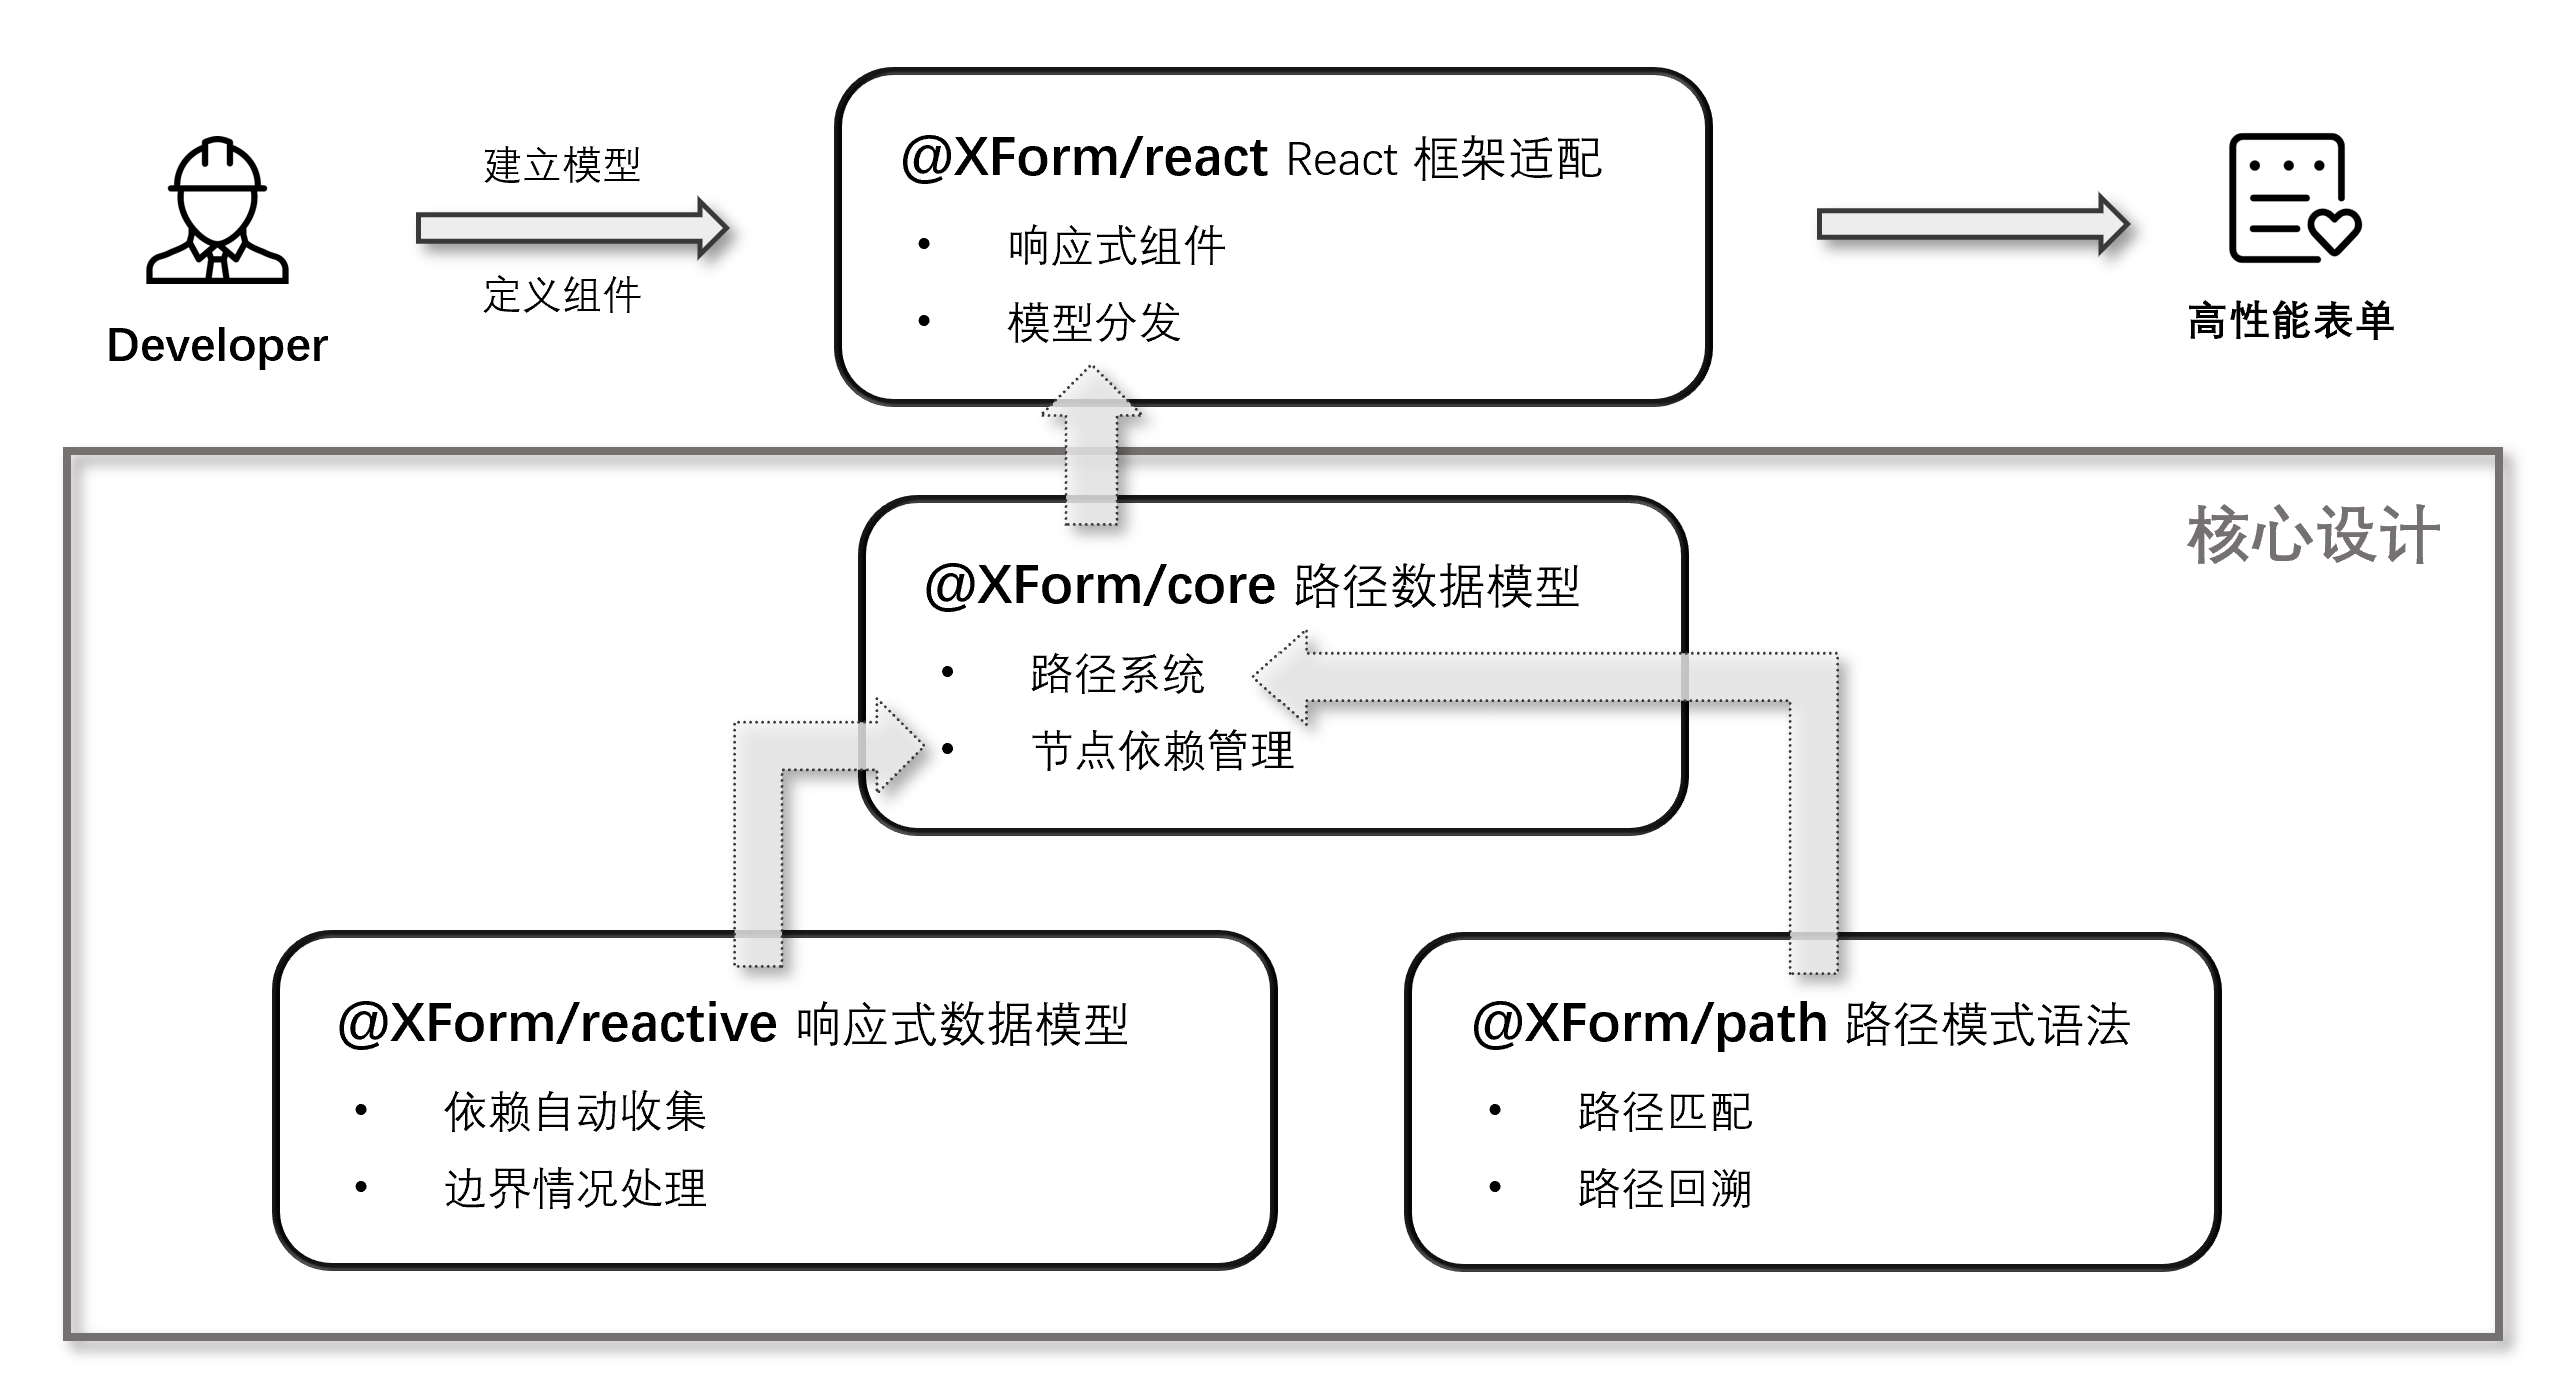
\includegraphics[width=\textwidth]{figure/overview.png}
    \caption{XForm 整体架构}
    \label{overview}
\end{figure}

在实践中,表单通常是围绕其模型设计进行开发的,而表单模型又以数据模型为核心构建\footnote{表单的核心目的是收集用户输入,天然地以目标输入数据为核心},因此数据模型的管理策略是表单解决方案应当考虑的核心问题。本文为了保证表单的渲染性能,首先基于模型驱动开发思想\cite{selic2003pragmatics}\cite{pastor2008model}设计了一套高性能数据模型管理方案;同时,为了保证该方案表达复杂运算关系的能力,又在其基础上封装了一套路径系统和消息总线机制,提供了模型内节点间通信的能力,从而实现了模型内部任意节点之间的运算关系定义。

以上述数据模型管理方案为基础,本文自底向上地提出了一整套表单开发工具的设计方案,其整体架构如\hyperref[overview]{图1-1} 所示,内容主要包括:

\begin{itemize}
    \item \textbf{\xform{reactive}}:一种解决变量间一对一运算关系定义的数据模型管理方法以及对应的工具实现,可以高效地管理数据间的依赖关系,从根本上提升表单的渲染性能。为 \xform{core} 提供基础的依赖关系管理功能。
    \item \textbf{\xform{path}}:一种用于定义多字段间运算关系的路径语法解析器,用于解析特定的匹配模式语法,为上层的路径管理方法提供支持。为 \xform{core} 提供多字段依赖关系定义的语法支持。
    \item \textbf{\xform{core}}:一种解决多字段运算关系管理问题的结构化数据模型管理方法,便于开发人员快速定义数据模型以及多字段间的依赖关系,以提升开发效率。为 \xform{react} 提供包含变量定义和运算关系定义在内的数据模型管理功能。
    \item \textbf{\xform{react}}:对 React 框架进行适配,提供由数据模型管理到渲染框架的完整工具链,简化开发人员完成数据模型与组件绑定的流程,进一步提升开发效率,提升代码的可维护性。
\end{itemize}

\section{本文组织结构}

本文组织如下:

第二章主要介绍本工作的研究背景,首先介绍了前端开发相关的背景知识,包括原生 DOM API 开发和基于框架的开发方案;接着基于真实案例介绍了表单开发场景区别于一般前端开发的主要特征;然后介绍了原生表单开发方式的缺陷并简要介绍了几类相关工作。

第三章给出了一种表单开发场景的建模方法,并基于该方法深入地讨论了几类包含相关工作在内的表单开发解决方案在渲染性能和开发效率两方面的理论差异,最终通过分析相关工作的优势和设计缺陷,给出了一种同时兼顾渲染性能和开发效率的表单开发解决方案,并总结了实现该方案时需要解决的具体问题。

第四章给出了一种基于路径系统的响应式数据模型的设计方案,目的是从根本上解决表单数据模型变量之间的运算关系管理问题,首先,通过分析表单数据模型定义的需求,渐进地给出了三个依赖收集算法设计;其次,为了实现多字段依赖定义,本文设计了一套路径匹配语法;最终结合消息总线和路径系统,基于依赖收集算法实现了一个高性能数据模型管理工具 \xform{core}。

第五章给出了基于 \xform{core} 对 React 框架进行适配的表单开发工具设计方案,提供了响应式组件封装和基于路径上下文进行模型分发的基础功能,同时针对表单场景的特性给出了复合组件的声明式定义接口,最终实现了渲染性能极佳、能够大幅提升开发效率的表单开发工具 \xform{react}。

第六章通过设计一系列实验对本文给出的数据模型管理工具 \xform{core} 和表单开发工具 \xform{react} 进行了各方面的评估,验证了本文工作的有效性。

第七章对本文的工作进行了简单的总结,并对后续可以进一步探索的研究方向给出了一些建议。

\chapter{背景知识}

本章首先介绍前端开发的基础知识,包括早期使用基础的 DOM API 进行精准的页面元素操纵以实现交互的方式,以及目前企业内部广泛使用的基于前端开发框架进行组件化开发的方式,并重点介绍后者的标准开发流程。然后结合案例分析表单开发场景的复杂性来源,最后简要介绍目前该领域的相关工作。

\section{前端开发基础}\label{frontend-development-basic}

自 Web 技术诞生以来,网页开发已经经历过多次技术革新,随着需求的不断丰富和应用场景的扩展,以及 MVC 模式的广泛应用,Web 前端开发已经逐渐形成了其独有的技术体系\cite{pop2014designing},这套体系以原生 Web 前端开发的 DOM API 为核心,在此基础上,出于开发效率,代码可维护性等多方面考虑,开发人员通常会基于抽象层次更高的前端开发框架进行快速地、渐进式地项目开发\cite{xing2019research}。其中,从各大论坛的热门词汇统计结果来看,React 是目前前端开发领域最热门的开发框架\cite{frontend-frameworks-popularity}。

\subsection{原生 Web 前端开发}

Web 页面的信息载体是 DOM (Document Object Model,文档对象模型) \cite{wood1998document},通常使用 HTML 语言\cite{berners1995hypertext}进行描述,浏览器通过解析 HTML 文档的内容生成对应的 DOM 树,一般来讲,HTML 文档内定义的标签\footnote{例如:html, body, div, span 等}会按照其声明的层次结构对应到 DOM 树上的节点,并最终由浏览器渲染为静态的图形界面\cite{garsiel2011browsers}。

DOM API 是对 DOM 节点进行操作的接口标准,现代浏览器如 Chrome,Edge,Safari 都使用 JavaScript 语言实现该标准,因此开发人员可以通过 JavaScript 代码精准地操纵 DOM 节点,完成一系列复杂的事件监听,节点创建、修改、删除等操作以实现用户交互,使网页内容具备动态特性,样例代码如下:

\lstinputlisting[style=HTML-with-JavaScript,caption={点击按钮,将目标元素的文本替换为 “Hello World”},captionpos=b]{code/hello-world.html}

\subsection{基于框架的 Web 前端开发}

直接使用 DOM API 进行开发能够使开发者保持对网页内容最细粒度的控制能力,但缺陷也是显而易见的,因为缺少模块化的手段,代码风格各异,原生开发生产的代码通常与上下文强相关,可复用性较差,并且存在潜在的可靠性问题\cite{ocariza2013empirical}\cite{icse2015javascript-mvc};此外,随着项目需求规模的扩大,开发流程的增加,由于 DOM API 较低的抽象层次无法有效地组织数据状态和 UI 状态,开发效率也受到了极大限制。为了提升开发效率,降低风险,应用 MVC 模式来管理 DOM 节点的数据状态和 UI 状态,同时基于模块化思想提高代码的可重用性,就成为了开发人员的共识,大量前端开发框架也由此应运而生。

\subsubsection{MVC 模式}\label{mvc-pattern}

\begin{figure}[h]
    \centering
    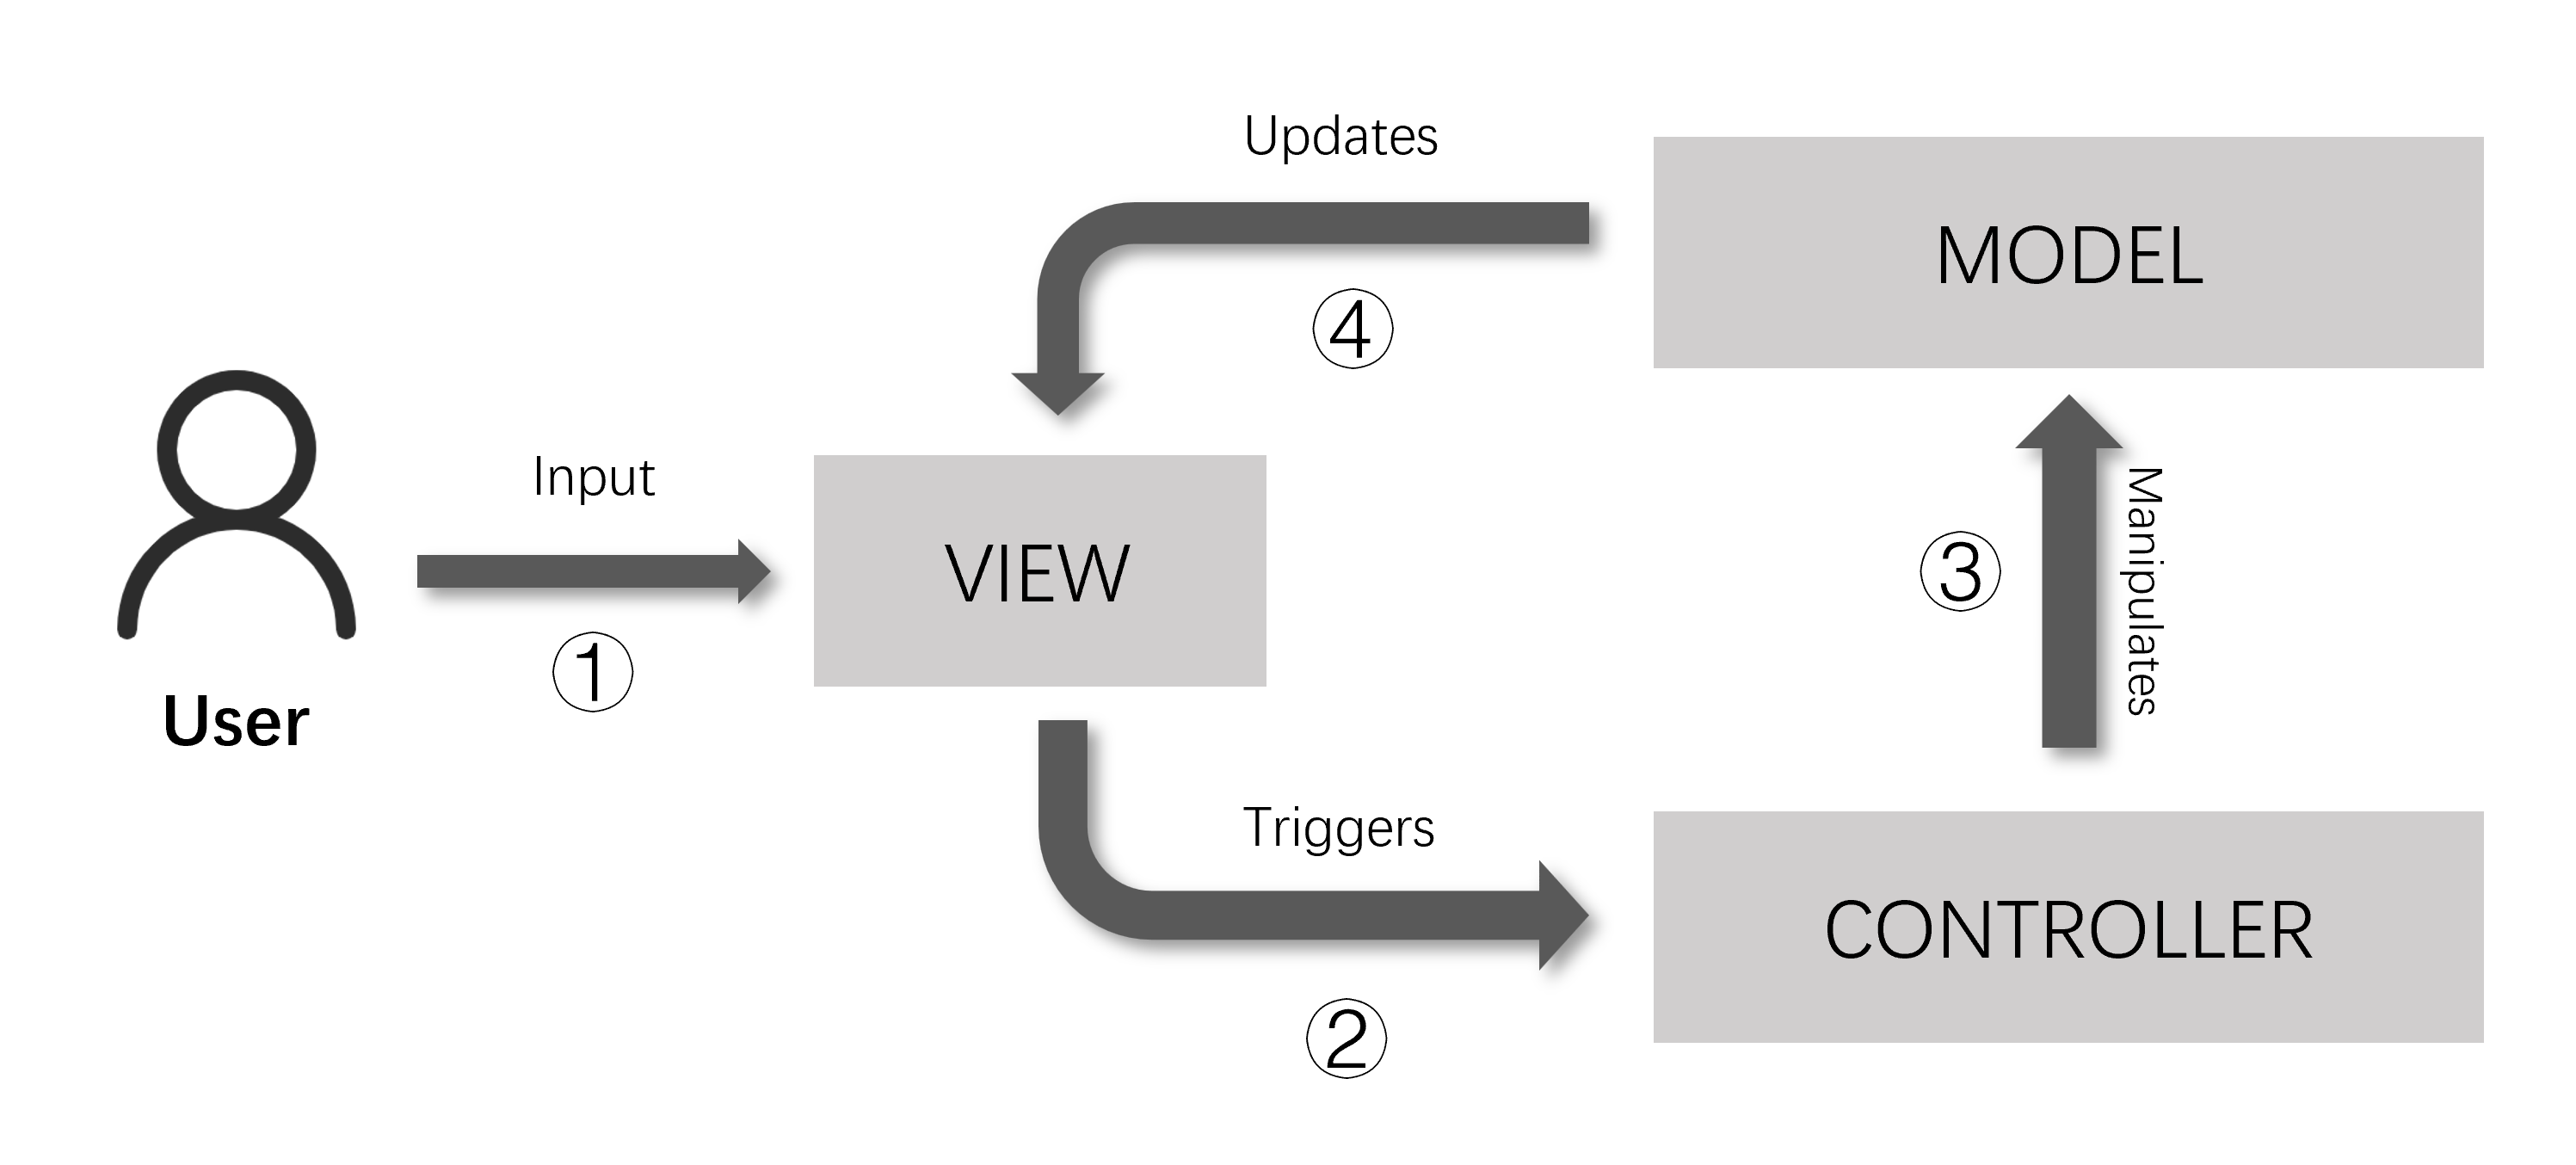
\includegraphics[width=0.7\textwidth]{figure/chapter-2/MVC-update.png}
    \caption{MVC 模式样例}
    \label{mvc-architecture-example}
\end{figure}

MVC (Model-View-Controller) 模式是一种广泛应用于图形化界面的软件设计模式,通过应用 MVC 模式,开发人员可以将代码逻辑拆分为模型、视图、控制器三类彼此关联的实例,有效地对 UI 交互逻辑和数据管理逻辑进行解耦,从而大幅提高代码的可维护性,早期的 MVC 模式是从 C/S 架构\footnote{Client/Server 架构,即客户端/服务端架构}中诞生的,由服务端完成模型的管理和控制器接口实现,客户端实现视图和控制器接口的调用\cite{leff2001web}。

随着 Web 技术的发展以及设备性能的提高,越来越多的计算任务可以在 Web 端完成,因此直接在 Web 端应用 MVC 模式来解决部分复杂 UI 的开发问题也变成了一个常见的解决方案\cite{taraghi2010simple}。一个典型的 MVC 模式设计大致如\hyperref[mvc-architecture-example]{图2-1} 所示\footnote{用户输入触发 View 中的回调,向 Controller 下达指令,引起 Model 数据变更,并最终更新 View},其中各部分的功能大致如下:

\begin{itemize}
    \item \textbf{Model(模型)}:管理目标应用的动态数据,接收来自 Controller 的数据变更事件,并在数据变更后通知 View 进行更新。
    \item \textbf{View(视图)}:UI 的具体展现形式,通常会在 View 中定义其在 Model 中关联的具体数据,并为特定的用户输入注册回调以触发 Controller 的响应。
    \item \textbf{Controller(控制器)}:接收来自 View 的指令,并相应地向 Model 发起数据变更事件。
\end{itemize}

\subsubsection{React 框架}\label{react-framework}

根据网站 statista 的统计\cite{frontend-frameworks-market-share},在基于 MVC 模式实现的前端开发框架中,React 是目前应用最广泛的,在全球范围内的使用率已经达到了 40\%。React 最早由 Facebook 公司开发并开源,时至今日,已经构建起了庞大的社区生态。React 框架的核心概念包含两部分,Virtual DOM 和 React 组件,通过两者的结合,React 框架不仅在渲染性能上有明显优势,也极大地提高了代码的可复用性,较原生开发方式大幅提升了开发效率。

\begin{figure}[h]
    \centering
    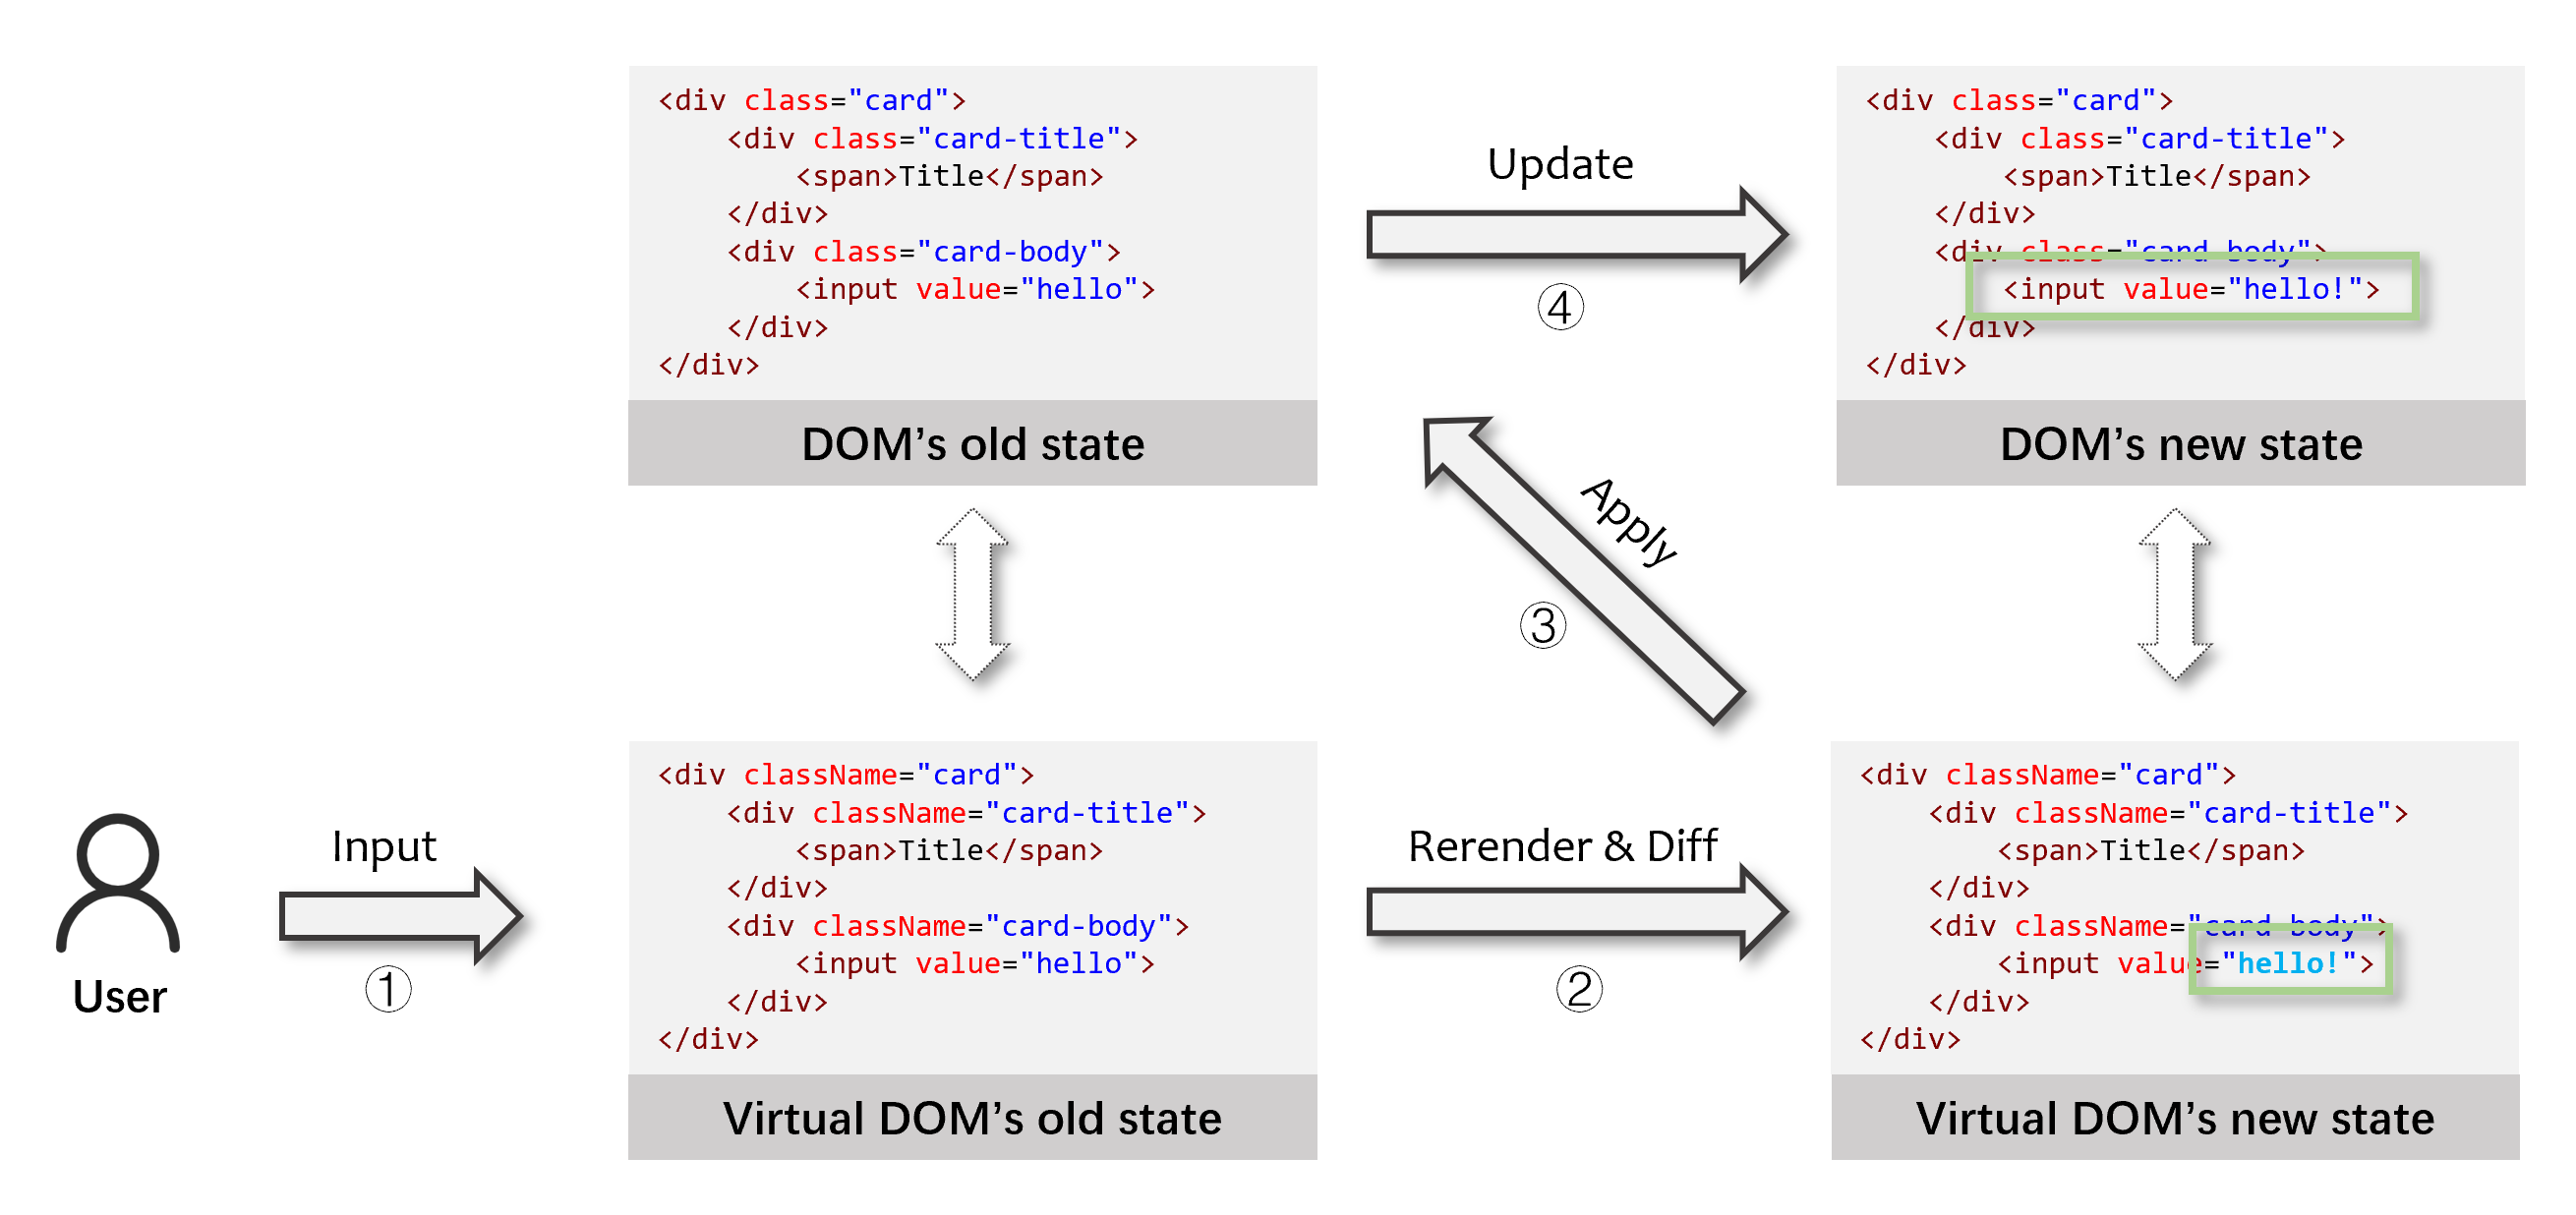
\includegraphics[width=\textwidth]{figure/chapter-2/VDOM-update.png}
    \caption{Virtual DOM 运行原理}
    \label{virtual-dom-runtime}
\end{figure}

Virtual DOM \footnote{虚拟化 DOM,以下简称 VDOM} 是一种被广泛应用于各种前端框架的设计思想\cite{virtual-dom},其核心思路是使用 JavaScript 对象在内存中维护一个 DOM 树的副本,开发人员直接控制 VDOM 的行为\footnote{对于特殊的交互需求,框架也会提供原生的 DOM API 接口,但是这种情况在实际开发过程中比较少见,一般用于适配基于原生 DOM API 实现的第三方 JS 库}。不同的前端框架在 VDOM 机制的设计上也存在差异,本文的研究针对 React 框架进行。

在 VDOM 发生变更时,React 框架通过对变更前后的 VDOM 执行 diff 算法来确认应该对哪些真实的 DOM 节点进行操作,diff 算法是一类用于计算 DOM 树间差异的算法\footnote{在实践中,通常将编辑距离作为 DOM 树间差异的主要参考变量},其基本思路是通过对新旧节点的一次广度遍历操作确定哪些节点发生了变更,需要如何新增/删除/修改节点来实现旧 DOM 树到新 DOM 树的转化,这种方法可以避免 DOM 操作本身的开销,从而提升渲染性能\cite{leithner2018domdiff}。一个典型的 diff 算法执行流程大致如\hyperref[virtual-dom-runtime]{图2-2} 所示。

React 框架通过 VDOM 机制完整地实现了 MVC 模式中 Controller 的功能,这一机制在大部分情况下对开发人员是透明的,因此开发人员可以重点考虑 Model 和 View 的设计,而无需关注 VDOM 的实现细节。进一步地,React 框架对此进行了关注点分离,并基于组件化思想\cite{heineman2001component}提供了 \textbf{React 组件}来帮助开发人员快速地定义可重用的渲染函数。在 React 组件的本质是一种可以同时管理视图(以下称 UI)和数据模型的 VDOM 节点生成函数,在具体实现时,UI 的定义方式大致与 HTML 定义标签的方式相同,数据模型管理接口则按照不同的作用域分为以下两类:

\begin{itemize}
    \item \textbf{state}:组件的内部数据模型,用于管理只在组件内部受控的数据。
    \item \textbf{props}:组件的外部数据接口,用于管理在组件外部受控的数据,结合 state 使用可以实现父子组件之间的数据通信。
\end{itemize}

在实践中,要完整地实现一个 React 组件,通常需要在同一个组件函数内分别进行数据模型定义以及 UI\footnote{在 React 框架中也可以称作 UI 渲染模板}定义。其中,数据模型定义要根据目标数据的作用域进行区分,内部数据使用 state 定义,外部传入的数据则使用 props 定义;视图定义则包含标签声明\footnote{和 HTML 语法中 DOM 标签定义的方式几乎一致,区别在于 React 支持以标签的形式对自定义组件进行复用}和数据注入\footnote{向目标标签注入 state 或 props 形式声明的变量}两部分内容。

React 组件运行时的动态渲染过程大致包括这样几个关键节点:当用户输入触发 state 变更时\footnote{props 的本质是祖先组件分发的 state,因此总会引起 state 的变更},React 框架会重新执行 state 声明对应的组件函数并生成新的 VDOM 节点及其子节点,触发 VDOM 的 diff 过程并最终完成真实 DOM 的更新,由于 diff 算法是基于广度递归遍历实现的,因此组件对应的 VDOM 节点深度越小,组件的子节点数量越多,渲染开销就越大,通常情况下,渲染开销会随着触发 state 变更的节点子树的规模线性增长。

\begin{figure}[h]
    \centering
    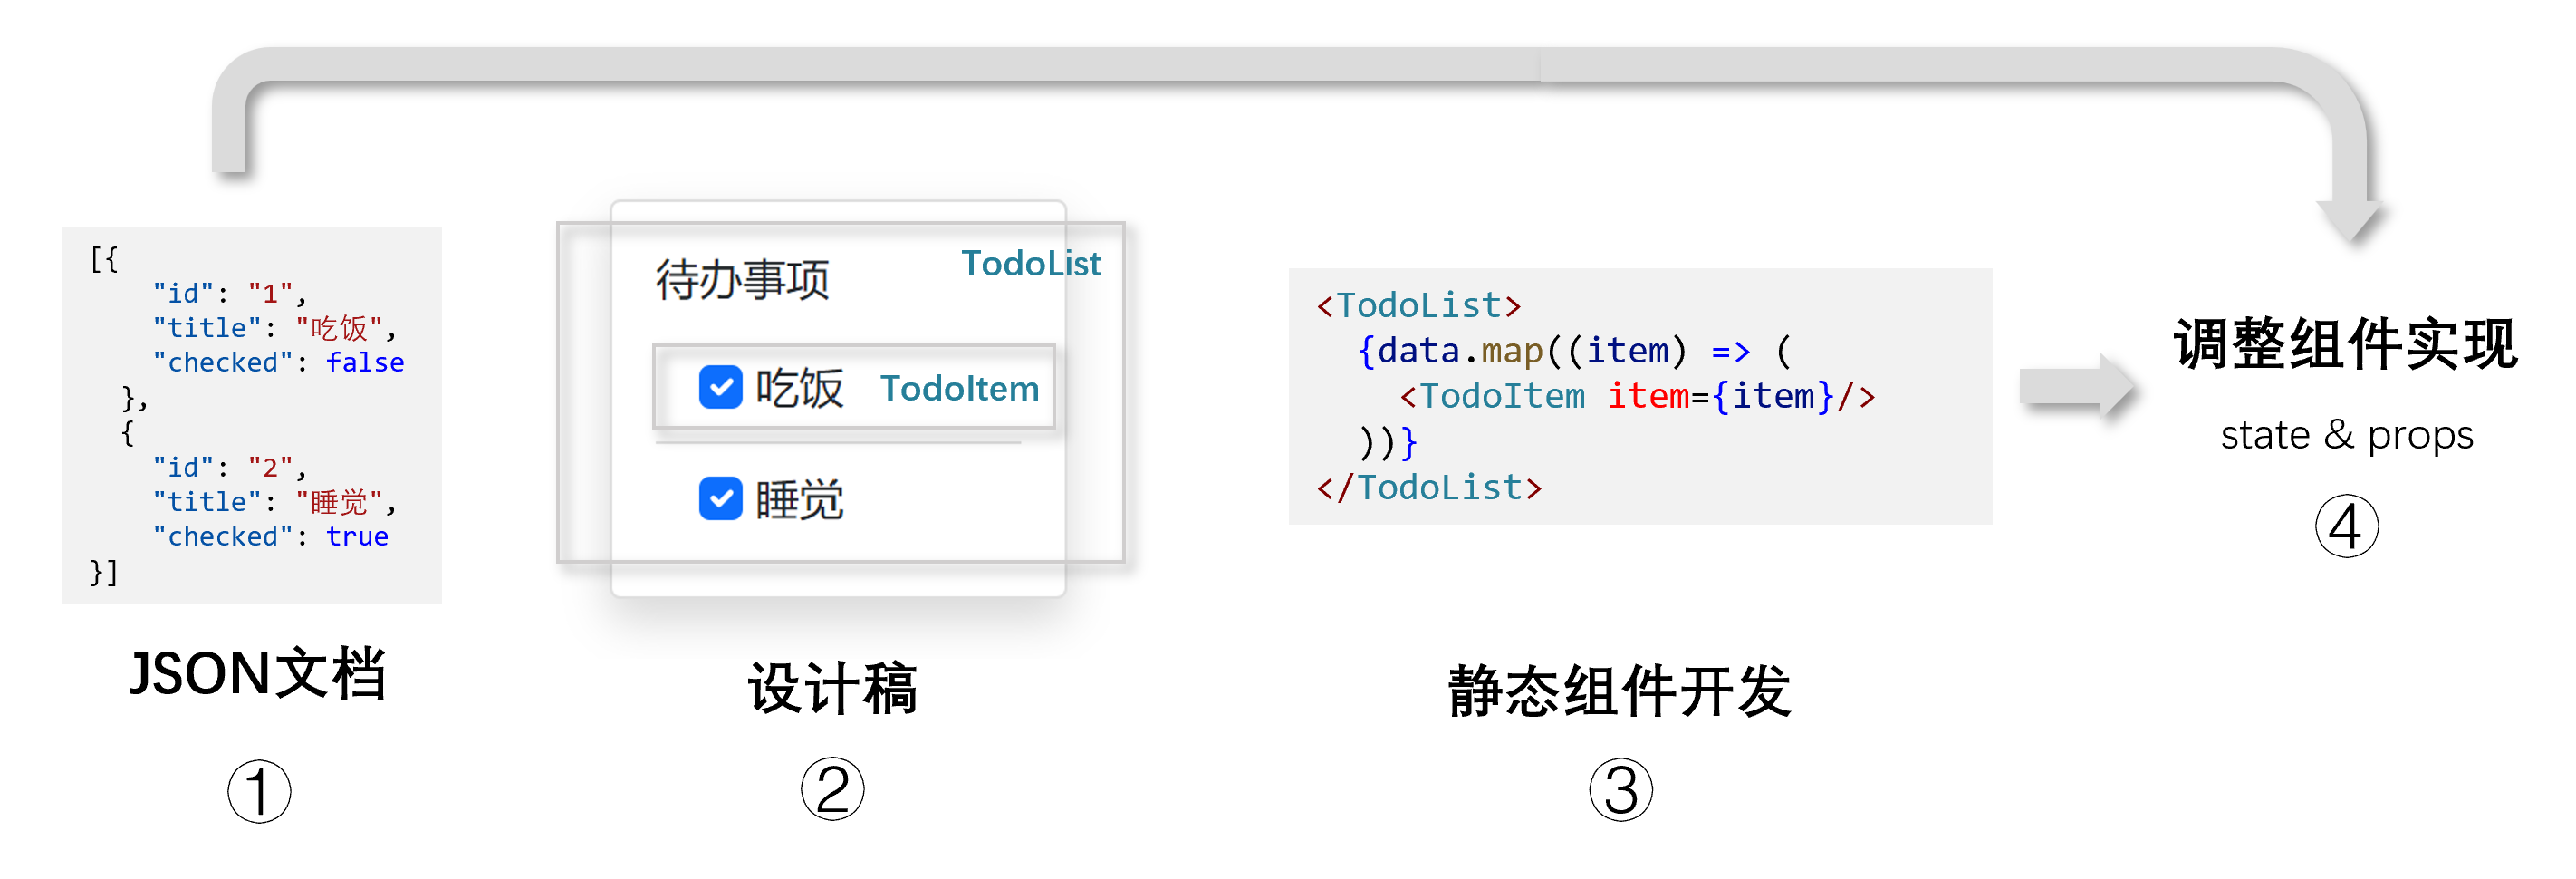
\includegraphics[width=\textwidth]{figure/chapter-2/react-component-development-pipeline.png}
    \caption{React 页面开发流程}
    \label{react-component-development-pipeline}
\end{figure}

编写代码进行 UI 开发的过程通常是十分耗时的\cite{schramm2010rapid}\cite{nguyen2015reverse}。和传统的 UI 开发流程相似,一个 React 项目的页面开发一般遵循由设计稿、数据接口到代码实现的流程\cite{myers1992survey},具体如下(如\hyperref[react-component-development-pipeline]{图2-3} 所示):

\begin{enumerate}
    \item 通过事先的业务需求沟通确定前端获取的 JSON\footnote{JavaScript Object Notaion,一种轻量级的数据描述语言,广泛应用于 Web 的数据传输\cite{json}} 数据格式\cite{nurseitov2009comparison}。
    \item 设计人员给出设计稿,开发人员根据设计稿划分组件的层次关系。
    \item 开发人员开发静态组件,调整具体实现以匹配设计稿。
    \item 出于提升渲染性能的考虑,开发人员需要尽可能地避免在 state 中管理大量的数据模型,根据业务需求确定 state 和 props 的最小集合并补充其声明,以及可能的计算逻辑\footnote{例如:定时逻辑,数据间的运算关系,网络请求}。
\end{enumerate}

在实际的生产中,由于业务需求和设计稿的变动,以及对后续业务扩展性的考虑,往往需要多次重复上述流程以实现目标组件,这也意味着开发人员需要反复地对 state 和 props 的声明做出调整,组件的嵌套层级越深,数据间的依赖关系越复杂,需要调整的组件也就越多,对于数据模型规模较大,且数据间存在复杂运算关系的大型页面组件来说,这种流程会极大地拖慢开发效率,而表单恰好就是集中了大规模数据模型和数据间复杂运算关系典型场景。

\section{表单开发场景}\label{form-development-scene}

表单是前端开发的一个重要场景,不同于大部分用户日常浏览网页时接触的表单,企业内部的表单由于其复杂的业务系统和交互需求设计,需要开发大量基础组件,并且针对表单中每一个字段实现复合组件,同时,表单内的数千个变量以及这些变量间存在的大量的依赖关系,导致表单开发的复杂性急剧提升。

以阿里集团考拉海购业务线的系统为例,表单作为开发人员和运营人员沟通的媒介,需要尽可能地将业务系统提供的接口以 UI 交互的方式呈现出来,降低接口的使用门槛,从而向运营人员开放更多的能力。

通常情况下,表单需要考虑如下几类交互设计需求\cite{bargas2007usable}\cite{bargas2011working}\cite{bargas2010simple}:

\begin{itemize}
    \item 基础输入组件,例如:文本输入框、单选框、多选框、开关。
    \item 基础容器组件,例如:卡片、分页、折叠面板。
    \item 布局方式,例如:列式布局、行内布局。
    \item 字段的描述信息,例如:标题、输入提示、输入描述。
    \item 字段的校验信息,例如:最大值、最小值、数值区间、正则校验、后端校验。
    \item 字段的统计信息,例如:部分字段的校验告警信息数量。
\end{itemize}

这些交互设计需求具体到实现细节上还需要开发人员和设计人员进行协商,对于复杂的表单模型,开发代价不容忽视。



\begin{table}[H]
    \centering

    \begin{threeparttable}
        \small
        \begin{tabular}{|lll|cccc|}
            \hline
            \multicolumn{3}{|c|}{数据模型}                  & \multicolumn{1}{c|}{输入组件}                   & \multicolumn{1}{c|}{容器组件}                    & \multicolumn{1}{c|}{布局方式}              & 依赖关系数量                                                               \\ \hline
            \multicolumn{3}{|l|}{\begin{tabular}[c]{@{}l@{}}基础信息\\ Object\end{tabular}} & \multicolumn{1}{c|}{无}                         & \multicolumn{1}{c|}{Card}                        & \multicolumn{1}{c|}{列式}                  & 13                                                                         \\ \hline
            \multicolumn{1}{|l|}{\multirow{7}{*}{}}         & \multicolumn{2}{l|}{\begin{tabular}[c]{@{}l@{}}ID\\ String\end{tabular}}  & \multicolumn{1}{c|}{Input}                       & \multicolumn{1}{c|}{Item}                  & \multicolumn{1}{c|}{行内}                  & 3                             \\ \cline{2-7}
            \multicolumn{1}{|l|}{}                          & \multicolumn{2}{l|}{\begin{tabular}[c]{@{}l@{}}部署时间\\ Object\end{tabular}}  & \multicolumn{1}{c|}{\multirow{3}{*}{TimePicker}} & \multicolumn{1}{c|}{\multirow{3}{*}{Item}} & \multicolumn{1}{c|}{\multirow{3}{*}{行内}} & \multirow{3}{*}{2}            \\ \cline{2-3}
            \multicolumn{1}{|l|}{}                          & \multicolumn{1}{l|}{\multirow{2}{*}{}}          & \begin{tabular}[c]{@{}l@{}}开始时间\\ String\textless{}Date\textgreater{}\end{tabular}                        & \multicolumn{1}{c|}{}                      & \multicolumn{1}{c|}{}                      & \multicolumn{1}{c|}{}     &   \\ \cline{3-3}
            \multicolumn{1}{|l|}{}                          & \multicolumn{1}{l|}{}                           & \begin{tabular}[c]{@{}l@{}}结束时间\\ String\textless{}Date\textgreater{}\end{tabular}                        & \multicolumn{1}{c|}{}                      & \multicolumn{1}{c|}{}                      & \multicolumn{1}{c|}{}     &   \\ \cline{2-7}
            \multicolumn{1}{|l|}{}                          & \multicolumn{2}{l|}{\begin{tabular}[c]{@{}l@{}}上线时间\\ Object\end{tabular}}  & \multicolumn{1}{c|}{\multirow{3}{*}{TimePicker}} & \multicolumn{1}{c|}{\multirow{3}{*}{Item}} & \multicolumn{1}{c|}{\multirow{3}{*}{行内}} & \multirow{3}{*}{3}            \\ \cline{2-3}
            \multicolumn{1}{|l|}{}                          & \multicolumn{1}{l|}{\multirow{2}{*}{}}          & \begin{tabular}[c]{@{}l@{}}开始时间\\ String\textless{}Date\textgreater{}\end{tabular}                        & \multicolumn{1}{c|}{}                      & \multicolumn{1}{c|}{}                      & \multicolumn{1}{c|}{}     &   \\ \cline{3-3}
            \multicolumn{1}{|l|}{}                          & \multicolumn{1}{l|}{}                           & \begin{tabular}[c]{@{}l@{}}结束时间\\ String\textless{}Date\textgreater{}\end{tabular}                        & \multicolumn{1}{c|}{}                      & \multicolumn{1}{c|}{}                      & \multicolumn{1}{c|}{}     &   \\ \hline
            \multicolumn{3}{|l|}{\begin{tabular}[c]{@{}l@{}}页面排期\\ Object{[}{]}\end{tabular}} & \multicolumn{1}{c|}{无}                         & \multicolumn{1}{c|}{Tab}                         & \multicolumn{1}{c|}{列式}                  & 0                                                                          \\ \hline
            \multicolumn{1}{|l|}{\multirow{4}{*}{}}         & \multicolumn{2}{l|}{\begin{tabular}[c]{@{}l@{}}页面外链\\ Object\end{tabular}} & \multicolumn{1}{c|}{无}                          & \multicolumn{1}{c|}{Collapse}              & \multicolumn{1}{c|}{列式}                  & 0                             \\ \cline{2-7}
            \multicolumn{1}{|l|}{}                          & \multicolumn{1}{l|}{\multirow{3}{*}{}}          & \begin{tabular}[c]{@{}l@{}}外链渠道\\ String{[}{]}\end{tabular}                       & \multicolumn{1}{c|}{Checkbox}              & \multicolumn{1}{c|}{Item}                  & \multicolumn{1}{c|}{行内} & 6 \\ \cline{3-7}
            \multicolumn{1}{|l|}{}                          & \multicolumn{1}{l|}{}                           & \begin{tabular}[c]{@{}l@{}}微信分享样式\\ Object\end{tabular}                       & \multicolumn{1}{c|}{定制组件}              & \multicolumn{1}{c|}{Divider}               & \multicolumn{1}{c|}{列式} & 1 \\ \cline{3-7}
            \multicolumn{1}{|l|}{}                          & \multicolumn{1}{l|}{}                           & \begin{tabular}[c]{@{}l@{}}QQ分享样式\\ Object\end{tabular}                       & \multicolumn{1}{c|}{定制组件}              & \multicolumn{1}{c|}{Divider}               & \multicolumn{1}{c|}{列式} & 1 \\ \hline
        \end{tabular}


        \begin{tablenotes}
            \item [1] 数据模型定义分别包含其关键字 Key 以及类型两部分
            \item [2] 数据模型类型与 JSON 的基本类型对应,Object 表示 Key-Value 形式的键值对类型,[] 表示数组类型
            \item [3] String<T> 表示数据的存储类型为字符串,逻辑类型为 T
            \item [4] 略去涉密内容,仅保留常见字段
        \end{tablenotes}

        \normalsize
    \end{threeparttable}

    \caption{考拉海购业务表单模型案例}
    \label{kaola-activity-configuration-form-model}
\end{table}

以下案例来自考拉海购业务线的某个真实系统\footnote{本文作者已和考拉海购就这部分数据披露达成了一致,由于部分内容涉密,因此文中给出的数据并不是完全准确的数值,仅用于描述大致规模},其部分表单模型设计如\hyperref[kaola-activity-configuration-form-model]{表2-1} 所示。完整的模型包含 70+ 个字段,为了实现各类交互需求,其变量规模为 2000+ 个,不考虑基础组件的开发代价,该表单的开发周期约为 20 个工作日,日常维护需要 3 - 15 个工作日,该时长与维护时受影响的变量规模有关,同等规模的表单在考拉海购业务线内部还有若干个,并且随着内部系统的功能升级、接口变更,表单的实现也需要不断调整,一般来说,平均每周就会产生一组与表单相关的需求。

如前文所述,使用 state 和 props 分别管理内部和外部数据的数据模型管理机制,在面对数据规模较大以及数据间运算关系较复杂的场景时,会极大地拖累开发效率,接下来本文将进一步解释表单开发过程中组件的管理方式,然后用两个实际的需求变更案例来说明 state \& props 机制是如何影响表单组件开发效率的。

在进行表单字段\footnote{即表单数据模型中的数据项,例如:“基础信息” 字段,“ID” 字段}对应组件的开发时,出于对代码可维护性的考量,表单字段与组件声明的数量通常不是一一对应的,原因很简单,一个字段要实现包括容器、布局、输入、显隐状态、可编辑状态、信息反馈在内的所有交互需求,如果把这些功能全部集成到一个组件中,显然违背了软件设计的单一职责原则\cite{martin2003agile}\footnote{这意味着即使字段的 UI 设计仅存在很小的差异,也需要重复书写大量组件代码,严重降低代码的可维护性}。

因此,在实践中,开发人员通常会将功能细分,实现一系列基础组件,进而通过逐层复用的方式来实现字段对应的复合组件,层级的增长也意味着 state 和 props 声明数量的增长\footnote{props 是通过父组件注入的方式向子组件分发的,只要使用组件,就需要逐个地完成每个 props 属性的注入},以 “微信分享样式” 字段为例,其组件层级大致如\hyperref[weixin-share-style]{代码2.2} 所示:

\lstinputlisting[label={weixin-share-style},style=component-example-style,caption={“微信分享样式” 组件层级},captionpos=b]{code/chapter-2/weixin-share-style.tsx}

当需求变更,需要在表单模型中新增(或删除、修改)数据间的运算关系时,相关的数据声明就必然要在 state 和 props 之间切换,开发人员也需要相应地修改声明代码,而这个过程并不是简单的文本替换能完成的,例如,对于如下 state 声明:

\lstinputlisting[style=component-example-style,caption={“微信分享样式” 组件层级},captionpos=b]{code/chapter-2/complex-initial-state.js}

由于需求变更,需要将数组项内部的 textTitle 作为外部数据接口传入,考虑到其嵌套的层级过深,如果整体替换整个 state 的声明就势必要调整大量组件的代码实现,甚至渲染性能也会受影响,性能调优又需要花费额外的代价。为了降低修改代价,一个比较常见的应对方式是为该字段取一个别名(alias),从而只需要修改其相关的部分组件的接口声明。当然,这种方式也是有代价的,大量别名的引入会极大地降低代码的可读性,也会提高后续维护的成本\cite{aldrich2002alias}。

具体来讲,引入大量别名来实现数据的作用域变更,会使得开发人员无法高效地确定数据的具体来源,因此开发人员需要谨慎地对待相关变量的每个组件层级的接口声明,逐个地查看并修改相关字段组件层级的实现,受影响的字段数量越多,需要修改的组件数量也就越多,开发周期也越长。这一点在新需求涉及到变量间的运算关系时尤其明显。以下是考拉海购案例表单日常开发过程中两个真实的需求变更案例。

\begin{itemize}
    \item 以表单模型中的 “XX分享样式” 字段为例\footnote{完整的模型包含约 9 个社交平台的分享样式},自根节点开始,封装这些字段对应的组件大致分为 4 \textasciitilde 10 个层级。在早期的模型设计方案,“XX分享样式” 的所有变量都直接维护在其 state 中。\\而随着业务调整,需要在模型中新增 “外链渠道” 字段,用户操作时仅显示 “外链渠道” 中已选中的社交平台对应的分享样式。\\为了实现这一需求,开发人员要自 “页面外链” 字段对应的组件开始调整约数十个组件的 state 和 props 声明以及和这些声明相关的所有运算代码,同时还需要讨论确定采用哪种数据传递方式,可能的方式有:1. 由 “页面外链” 字段对应的组件将 “外链渠道” 字段对应的当前值声明到 state 中,并注入所有子组件的 props,由子组件判断是否隐藏;2. 由 “页面外链” 字段对应的组件将 “XX分享样式” 的显示隐藏属性声明到 state 中,直接控制相关字段的显隐状态。\\最终这样一个需求会耗费 3 个工作日的时间。
    \item 早期的表单设计只在各个字段内部实现了独立的校验机制,完全基于 state 在每个字段对应的复合组件内部进行校验信息的管理,但是随着字段数量的增加,页面承载的内容逐渐无法在同一个视窗内展示,因此需要通过分栏分页等手段隐藏部分内容来提升交互体验,但随之而来的问题是,用户无法得知这部分隐藏内容的校验结果,只能逐个地浏览表单项来查看输入是否正确,这大大降低了表单交互的效率。\\基于上述原因,表单需要在常驻的内容上呈现必要的校验信息,以达到快速定位错误的目的,例如在 “基础信息” 字段对应的标题处展示其所有子节点总的错误数量。为了实现这一需求,开发人员要自 “基础信息字段” 开始调整其约 20 个子节点对应的约 100 个组件的 state 和 props 声明,参考前文所述的需求案例,受影响的运算代码也要对应地进行多次修改。\\最终这样一个需求大致会耗费 7 个工作日的时间。
\end{itemize}

通过对上述案例的分析可以得到一个初步结论:表单模型内部的变量间运算关系越复杂,使用原生 React API 进行数据管理的开发代价越大\footnote{实际上,假设不存在这类运算关系,那么所有的变量都可以通过 state 在组件内部声明,开发人员也就无需为了一个需求大批量地修改组件的具体实现了}。

\section{相关工作}\label{related-work}

如前文所述,在表单模型内部变量存在大量运算关系的情况下,开发人员需要分别针对不同作用域的数据使用 state 和 props 实现表单的数据模型管理以进行渲染性能优化,这是限制表单开发效率的主要原因。如果存在一种统一接口的数据模型管理方式可以解决此类运算关系定义的问题,以替代 React 原生的数据模型管理方案,开发效率就应当能够得到显著提升。

相关工作围绕这一思路已经有了一些成熟的解决方案,并且在特定的表单开发场景下呈现了显著的开发效率提升,本文将针对以下三个典型的工作进行深入分析:

\begin{itemize}
    \item \textbf{react-jsonschema-form}\cite{react-jsonschema-form}:采用声明式语法进行组件复用和数据定义的表单开发工具。
    \item \textbf{react-final-form}\cite{react-final-form}:提供高性能数据模型管理的表单开发工具。
    \item \textbf{formily}\cite{formily}:对表单领域进行了深度建模的高性能表单开发工具。
\end{itemize}

三类工具的特性和具体的分析过程将结合本文给出的表单开发建模方法在\hyperref[problem-analysis]{第三章}中详细介绍。

\chapter{问题分析}\label{problem-analysis}

考虑到对于不同的表单开发解决方案,其渲染过程和具体的开发代价都存在差异,为了深入地探究它们的具体差异和设计上的缺陷,给出进一步的优化方案,本文对表单开发领域进行了全面建模。

结合 MVC 模式的思想进行分析,表单的本质实际上是数据模型和 UI 模型的结合。开发人员首先需要设计表单的数据模型和 UI 模型,建立数据模型与 UI 模型之间的逻辑关联,明确数据模型内部各个变量之间可能存在的运算关系,并最终使用特定的 API 完成具体的模型定义。在 React 框架下,UI 模型恰好与组件机制相对应,下文将统一使用组件来表达 UI 模型。

\section{问题建模}\label{problem-modeling}

考虑到在实践中,表单模型通常是基于原始的 JSON 格式数据设计的,天然地以树结构形式存在,因此本文参考 JSON-Schema\footnote{一种专门用于描述 JSON 数据结构的语法,通常用于定义数据约束以进行数据合法性校验} 语法将表单字段的树结构和字段相关的变量统一到一起\cite{pezoa2016foundations},以描述其数据模型的基础结构,并在此基础上通过建立有向图来描述字段内变量之间的运算关系。

在数据模型的基础上,参考 Botterweck 等人的工作\cite{botterweck2006model},本文针对数据模型和组件间的映射关系也进行了建模,以探索各类策略的理论差异。

如上文所述,在 React 框架下,表单模型设计的本质是数据模型和组件的结合,而数据模型又包含表单字段,字段内与组件相关的变量以及这些变量之间的运算关系,因此本文建模方案的关注点是字段、变量、组件三个部分以及三者之间的映射关系,具体方案如下:

\begin{itemize}
    \item \textbf{表单字段}:使用 
\includegraphics[height=1em]{figure/chapter-2/Node.pdf} 表示表单数据模型中的字段(记作 $Node$),
\includegraphics[height=1em]{figure/chapter-2/Tree_Edge.pdf} 表示字段的父子关系(父字段指向子字段)。
    \item \textbf{字段变量}:使用 
\includegraphics[height=1em]{figure/chapter-2/Attribute.pdf} 表示字段内的变量(记作 $Attr$),
\includegraphics[height=1em]{figure/chapter-2/Attribute_Edge.pdf} 表示字段与变量的从属关系(记作 $Node\$Attr$),
\includegraphics[height=1em]{figure/chapter-2/Dedenpency_Edge.pdf} 表示变量之间存在运算关系(运算结果指向依赖源,记作 $Dep_t=Node_x\$Attr_i\rightarrow Node_y\$Attr_j$)。此外,本文将使用
\includegraphics[height=1em]{figure/chapter-2/update_variable.png}来表示某变量的值发生了变化。
    \item \textbf{组件}:使用
\includegraphics[height=1em]{figure/chapter-2/Component.pdf} 表示特定的基础组件(记作 $Component$),
\includegraphics[height=1em]{figure/chapter-2/Component_Group.pdf} 表示复合组件(记作 $ComponentGroup = [Component_m,Component_n,\dots]$,简记作 $CG$),
\includegraphics[height=1em]{figure/chapter-2/Component_Edge.pdf} 表示字段与复合组件的映射关系(记作 $Node_x \Leftrightarrow ComponentGroup_x$),其中黑色字体对应组件名称,蓝色字体对应与之关联的字段变量,变量和基础组件的映射关系记作$Node_x\$Attr_y\Leftrightarrow Component_m$,
\includegraphics[height=1em]{figure/chapter-2/Component_Layer.pdf} 表示组件之间的层级关系(父组件指向子组件)。此外,本文将使用
\includegraphics[height=1em]{figure/chapter-2/update_component.png}来表示某基础组件进行了重新渲染。
\end{itemize}

考拉海购的案例表单模型可以通过上述方案建模为如\hyperref[entire-model]{图3-1} 所示的形式。需要强调的是,该建模方案仅面向表单模型的逻辑设计,在实际运行时,字段的层级关系,字段变量的管理方式,组件的层级关系,变量变化时组件的更新策略都取决于具体的实现策略。

\begin{figure}[h]
    \centering
    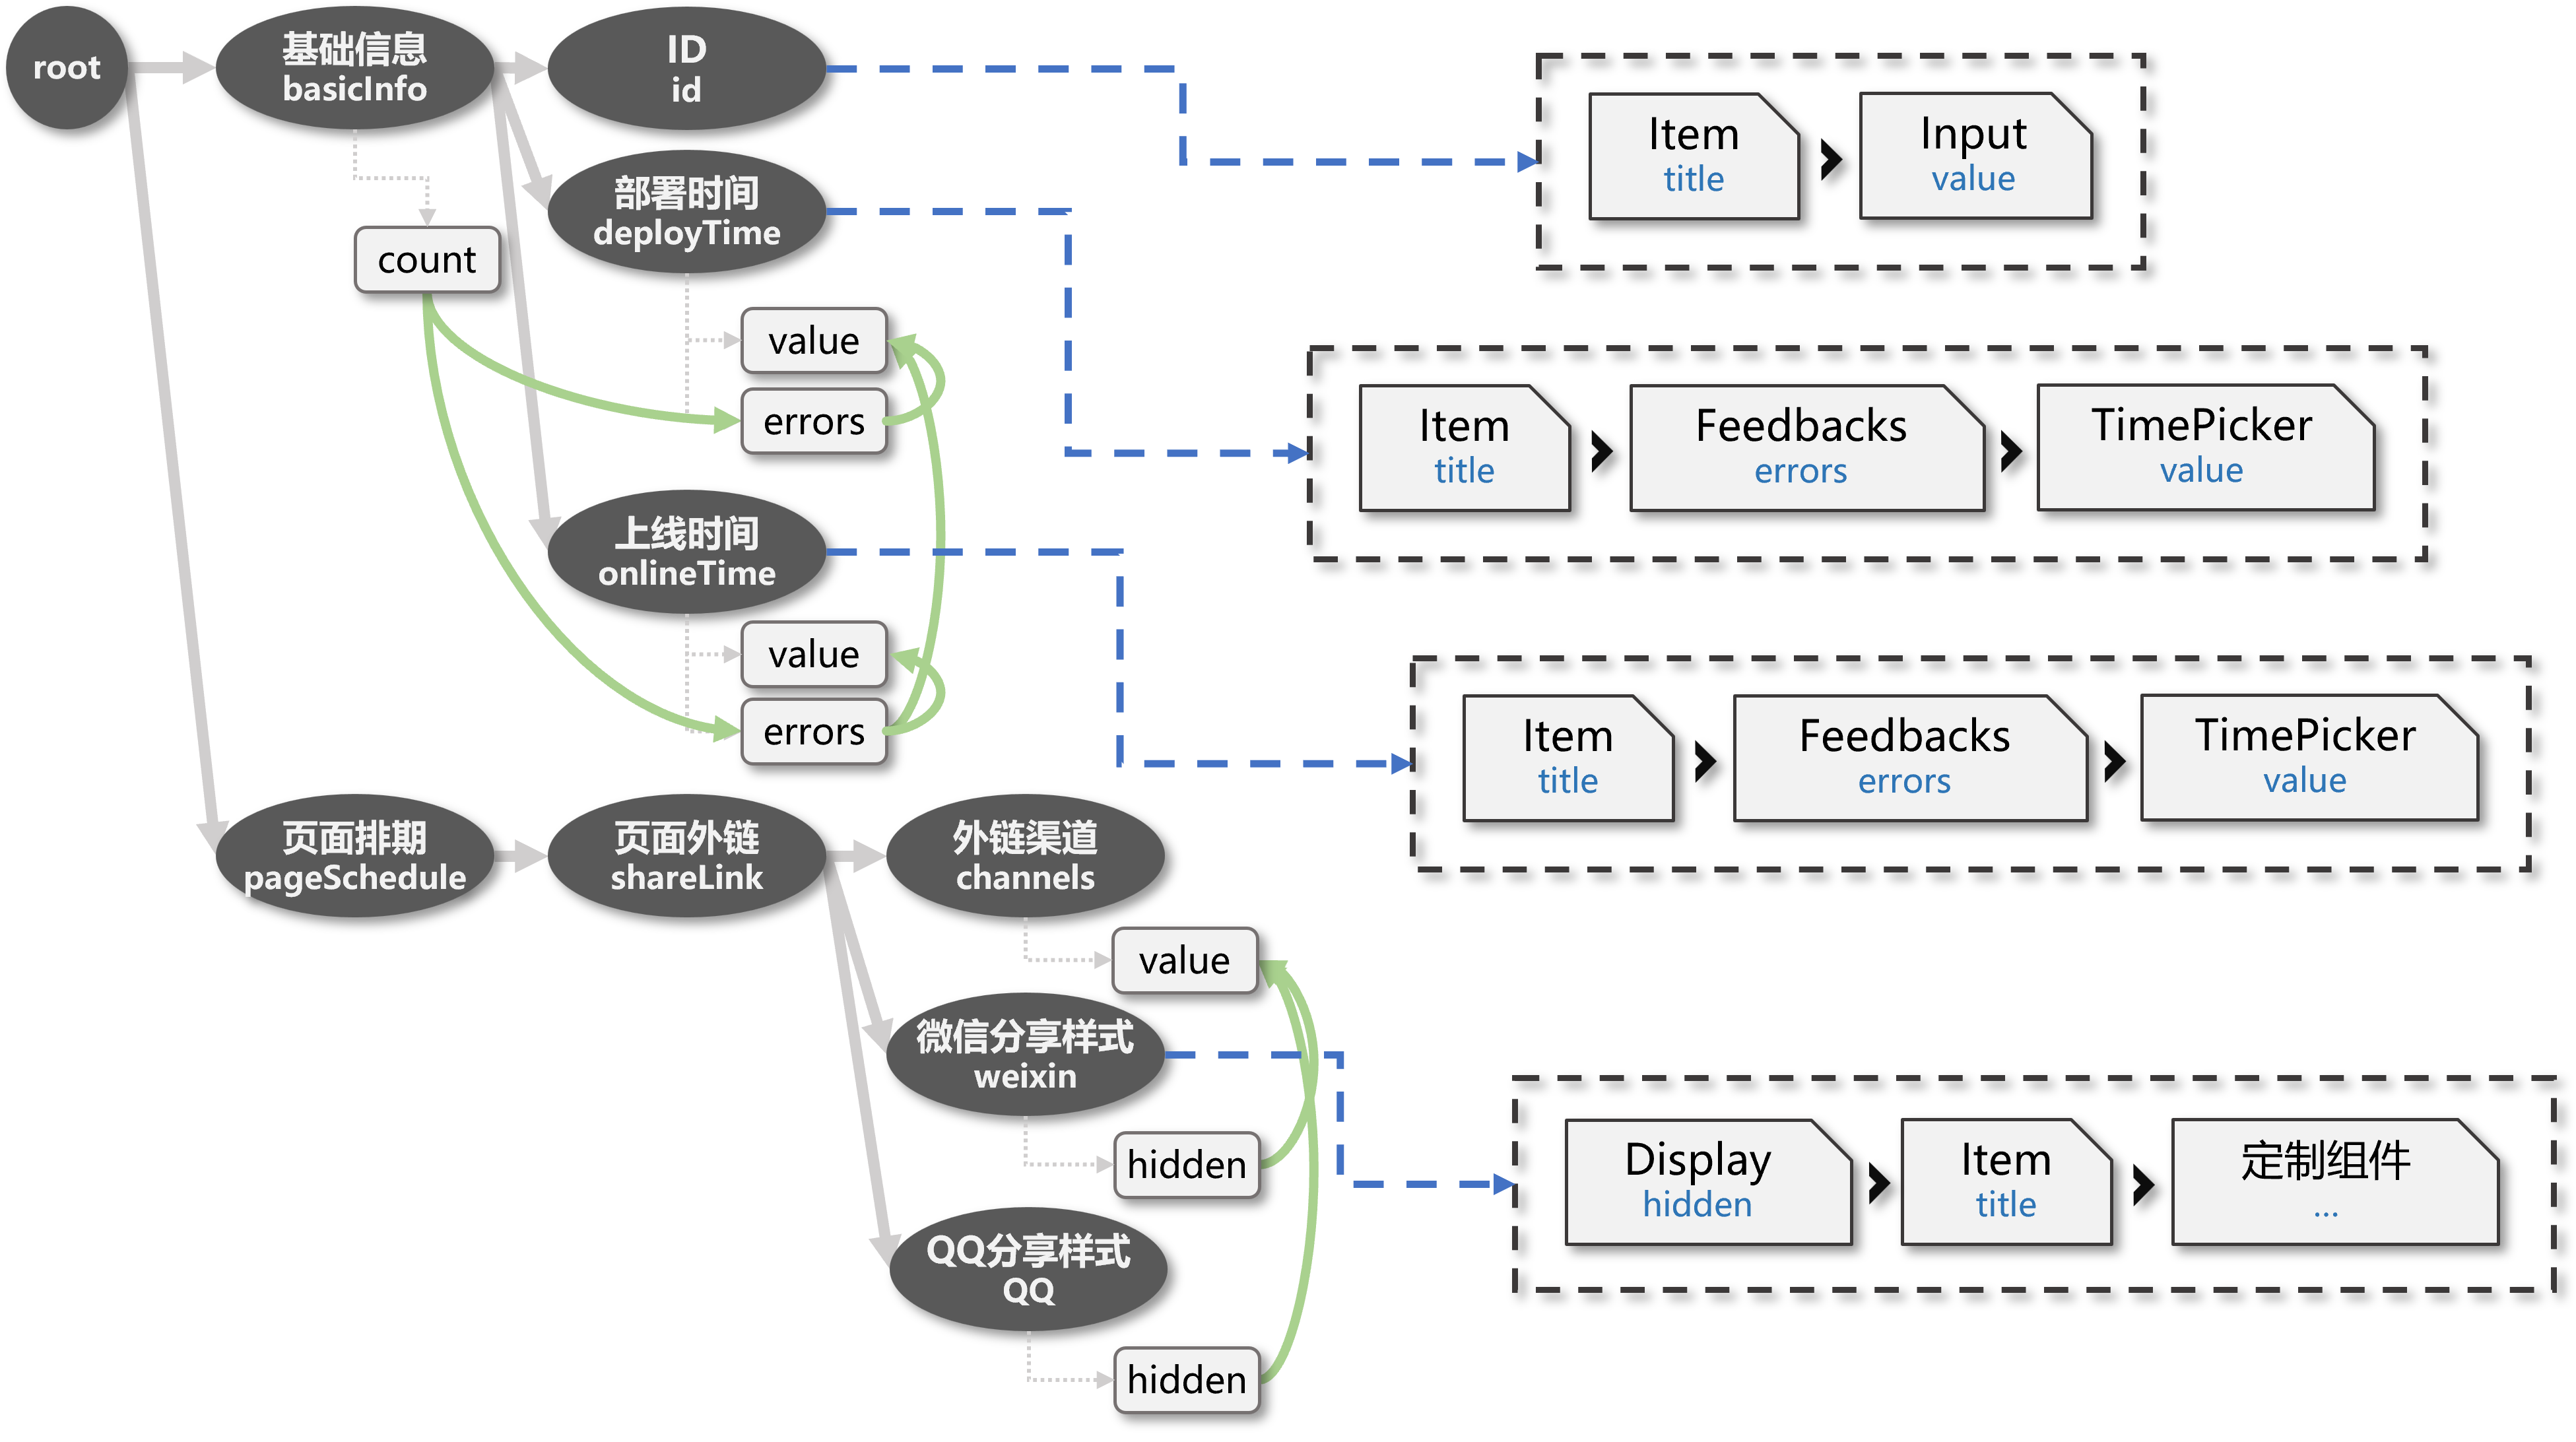
\includegraphics[width=0.9\textwidth]{figure/chapter-2/entire_model.png}
    \caption{考拉海购表单建模样例}
    \label{entire-model}
\end{figure}

此外,为了更好地区分运算关系的特征,本文对变量间运算关系进行了分类,下文将这类变量间运算关系称作\textbf{依赖关系}。结合考拉海购的案例来看,依赖关系可以分为三种基本类型,一对一依赖、一对多依赖、多对一依赖,具体说明如\hyperref[dependency-situations]{表3-1} 所示。

\begin{table}[H]
    \centering

    \begin{threeparttable}
        \small

        \begin{tabular}{|c|p{12cm}<{\centering}|}
            \hline
            类型       & 样例                                                                                               \\ \hline
            一对一依赖 & \textbf{上线时间}的值必须在\textbf{部署时间}当前值对应的时间段内,若该条件未满足,则生成校验错误信息 \\ \hline
            一对多依赖 & \textbf{基础信息}的 count 变量的值为所有子字段的校验错误信息的数量之和                        \\ \hline
            多对一依赖 & \textbf{微信分享样式}、\textbf{QQ分享样式} 仅在\textbf{外链渠道}存在相应的值时才可见               \\ \hline
        \end{tabular}

        \begin{tablenotes}
            \item [1] 样例均取自\hyperref[kaola-activity-configuration-form-model]{表2-1} 中的表单数据模型

        \end{tablenotes}

        \normalsize
    \end{threeparttable}

    \caption{表单变量依赖关系分类}
    \label{dependency-situations}
\end{table}

\section{相关工作分析}\label{related-work-analysis}

为了更精准地定位表单开发场景需要解决的问题,本文基于上述建模方案对已有工作在渲染性能和开发效率两方面进行了评估。

本文引入以下几个用于描述渲染开销计算过程的一些关键参数和方法:

\begin{itemize}
    \item 单个基础组件的平均渲染时间记作 $C$,单个依赖关系的平均计算时间记作 $D$,通常情况下,依赖关系的计算时间远小于组件渲染时 diff 算法的执行时间以及 DOM 更新的时间,即 $C\gg D$,因此若无特殊注明,否则默认依赖关系的计算时间对分析结果不产生影响。
    \item $get\_all\_child(Node_x)$:获取目标字段的所有子字段集合,返回 $\text{Set}\langle Node\rangle()$。
    \item $get\_neighbor(Node_x\$Attr_y)$:获取依赖关系指向目标字段变量的距离为 1 的字段集合(不包括 $Node_x$ 字段),返回 $\text{Set}\langle Node\rangle()$。
    \item $len(CG_x)$:获取目标复合组件包含基础组件的个数。
\end{itemize}

\subsection{原生 React 开发}

完全基于 state \& props 进行数据管理的原生 React 开发方式,其渲染开销与字段变量的数据接口声明位置相关,需要针对字段变量是否存在依赖关系、依赖关系对应变量所处的组件层级进行具体分析,一般来讲,任一字段变量 $Node_x\$Attr_y$ 变更时,其渲染时间的计算方式大致如下:

\begin{enumerate}
    \item 初始化渲染时间开销 $sum$。
    \item 累加字段 $Node_x$ 对应的复合组件及其子字段的复合组件重新渲染的代价 $sum=sum+C*\sum_{Node_i\in get\_all\_child(Node_x)}len(CG_i)$。
    \item 遍历 $get\_neighbor(Node_x\$Attr_y)$ 中的字段,重复步骤 2-3。
\end{enumerate}

例如,对于\textbf{上线时间}字段,当用户输入触发 value 变化时,由于依赖关系的存在,$onlineTime\$value > onlineTime\$errors > basicInfo\$count$ 需要依次变更,而 $value$ 和 $errors$ 处于同一字段内会被合并计算,最终\textbf{上线时间}对应的复合组件会进行一次渲染,\textbf{基础信息}对应的复合组件(以及子节点对应的所有复合组件)会进行一次渲染,总的渲染时间为 $O(C*(len(CG_{onlineTime})+len(CG_{basicInfo}))+len(CG_{id})+len(CG_{deployTime})+len(CG_{onlineTime}))$。

而对于\textbf{ID}字段,当用户输入触发 value 变化时,由于没有依赖关系的存在,其渲染时间为 $O(C*(len(CG_{id})))$

总的来讲,在使用原生 React 开发方案进行开发时,字段变量的依赖关系越多,跨越的层级越多,渲染时间就会越长。

而在具体实现时,原生 React 开发方式要求字段定义、变量定义、依赖关系定义、复合组件定义、实现字段和组件之间的映射关系(以下简称\textbf{字段与组件绑定}或\textbf{组件绑定})都需要开发人员手动实现,其中字段定义和变量定义还分为内部数据和外部数据两类,需要综合考虑需求场景以及渲染性能来选择合适的方案。

\subsection{全局覆盖策略}

\begin{figure}[h]
    \centering
    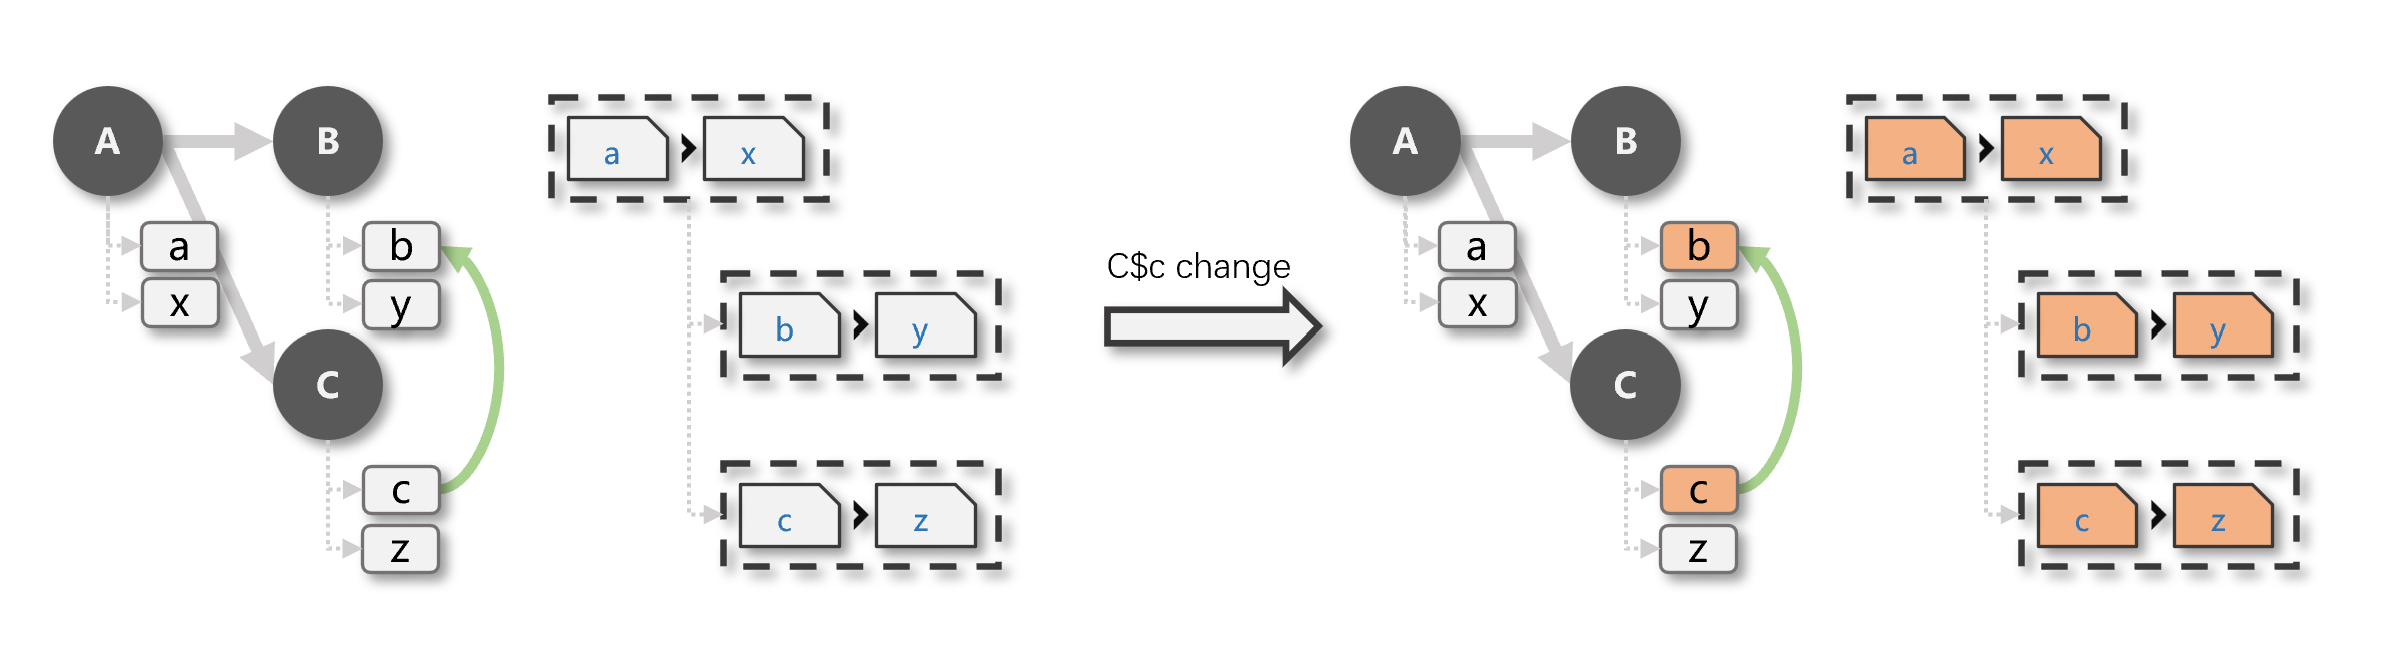
\includegraphics[width=0.9\textwidth]{figure/chapter-2/global-cover.png}
    \caption{全局覆盖策略运行效果}
    \label{global-cover}
\end{figure}

以 react-jsonschema-form 为代表的一类工具采用的是\textbf{全局覆盖}策略(参考\hyperref[global-cover]{图3-2}),其核心思路如下:

\begin{itemize}
    \item 将所有组件按照其对应的数据模型的层级组织成一棵组件树,在该组件树的根节点维护全局的数据模型以及所有变量间依赖关系。
    \item 该全局数据模型自表单组件树的根节点开始逐级进行分发,以实现字段和目标复合组件的关联。
    \item 当用户输入触发任一变量的变更时,所有的依赖关系都需要重新计算,得到新的数据模型,并直接覆盖掉旧的数据模型。
    \item 通过覆盖式地更新,新旧模型差异计算的代价直接转移到了 React 框架上,因此任意变量的变化都会使 React 框架从根节点开始执行一次 diff 算法,最终导致渲染开销与表单规模呈线性关系。
\end{itemize}

由于数据模型以覆盖的方式进行更新,因此任一字段变量变化时,都是从根节点开始进行一次组件更新,其渲染代价几乎相同,满足如下公式:

\begin{equation}
O(C*\sum_{Node_i\in Model}len(CG_i))
\end{equation}

即渲染代价与整个模型基础组件的数量成正比,或者说,与字段数量成正比,因此在模型规模较大的情况下,全局覆盖策略会导致渲染时间增加到明显影响用户交互的程度(以下称这种情况为存在渲染瓶颈),这导致全局覆盖策略只适用于规模较小的数据模型。

而在具体实现时,以全局覆盖策略实现的工具通常要求字段定义、变量定义、依赖关系定义、复合组件定义由开发人员手动实现;而组件绑定只需要简单的声明,具体的绑定过程由工具自动完成;同时,字段和变量统一以全局方式实现,省去了区分内部外部数据的过程,相较于原生 React 开发方式极大地简化了开发成本。

\subsection{模型切分策略}

\begin{figure}[h]
    \centering
    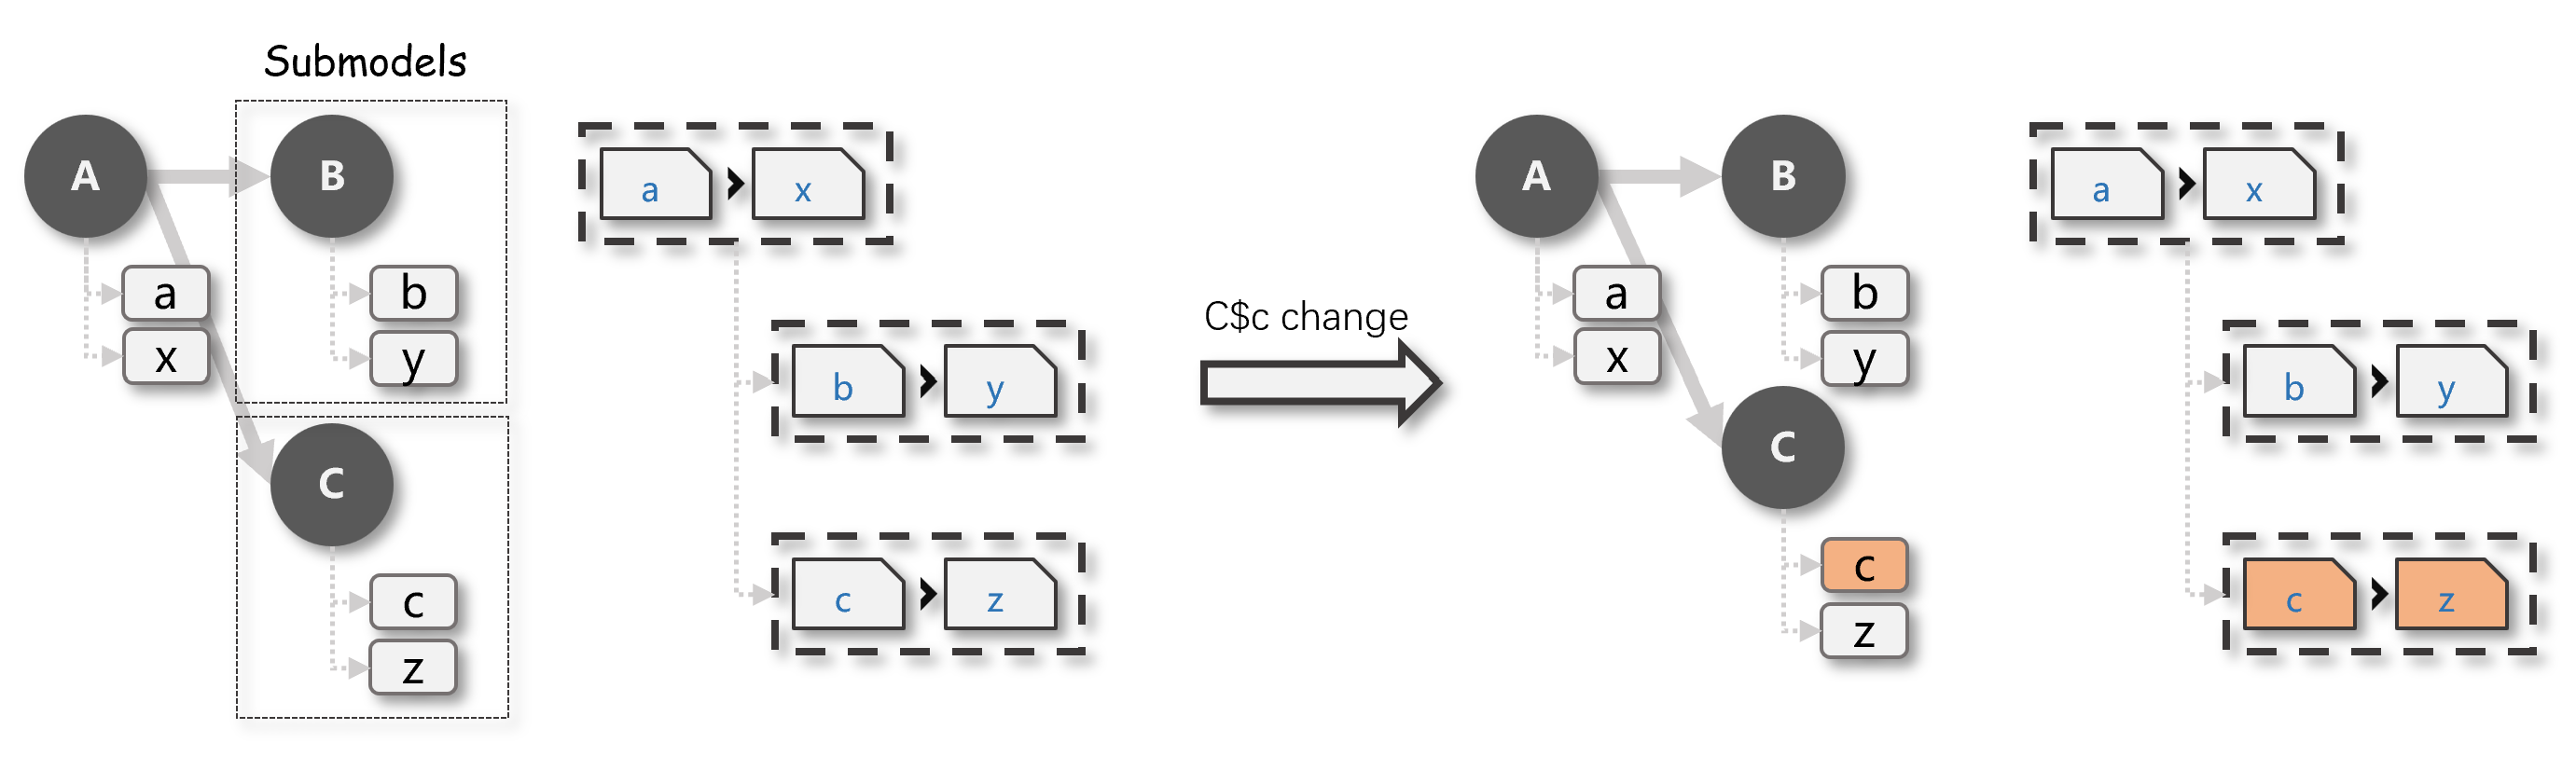
\includegraphics[width=0.9\textwidth]{figure/chapter-2/model-split.png}
    \caption{模型切分策略运行效果}
    \label{model-split}
\end{figure}

以 react-final-form 为代表的一类工具采用的是\textbf{模型切分}策略(参考\hyperref[model-split]{图3-3}),其核心思路是:将所有深度为 1 的模型字段切分成独立的子模型,在子模型内部依旧使用全局覆盖策略管理数据模型。

与全局覆盖策略相比,对于深度较小的原始模型来说,由于子模型之间相互独立,因此这种策略会有显著的性能提升,但代价是无法表达跨子模型的依赖关系;同时,对于深度较大的原始模型来说,随着单个子模型规模的增长,这种策略会逐渐退化到全局覆盖策略的性能开销。

模型切分通过为子模型独立地维护数据模型实现了分摊渲染开销的效果,例如,对于考拉海购的案例表单,分别为\textbf{基础信息}字段和\textbf{页面排期}字段独立地维护数据模型,则两者的渲染时间将分别为 $O(C*\sum_{Node_i\in Model_{basicInfo}}len(CG_i))$ 和 $O(C*\sum_{Node_i\in Model_{pageSchedule}}len(CG_i))$。

这种策略对于深度较小的模型具有显著的性能提升,但缺陷也是显而易见的,首先,它无法表达跨模型的依赖关系,应用场景受限,如果表单模型存在跨模型的依赖关系,就会退化到全局覆盖策略;其次,对于子字段规模较大的表单模型,它依然存在性能瓶颈,所以模型切分策略也只适用于规模较小的数据模型。

而在具体实现时,以模型切分策略实现的工具,其接口设计与全局覆盖策略基本一致,这里不再赘述。

\subsection{模型一维化策略}

\begin{figure}[h]
    \centering
    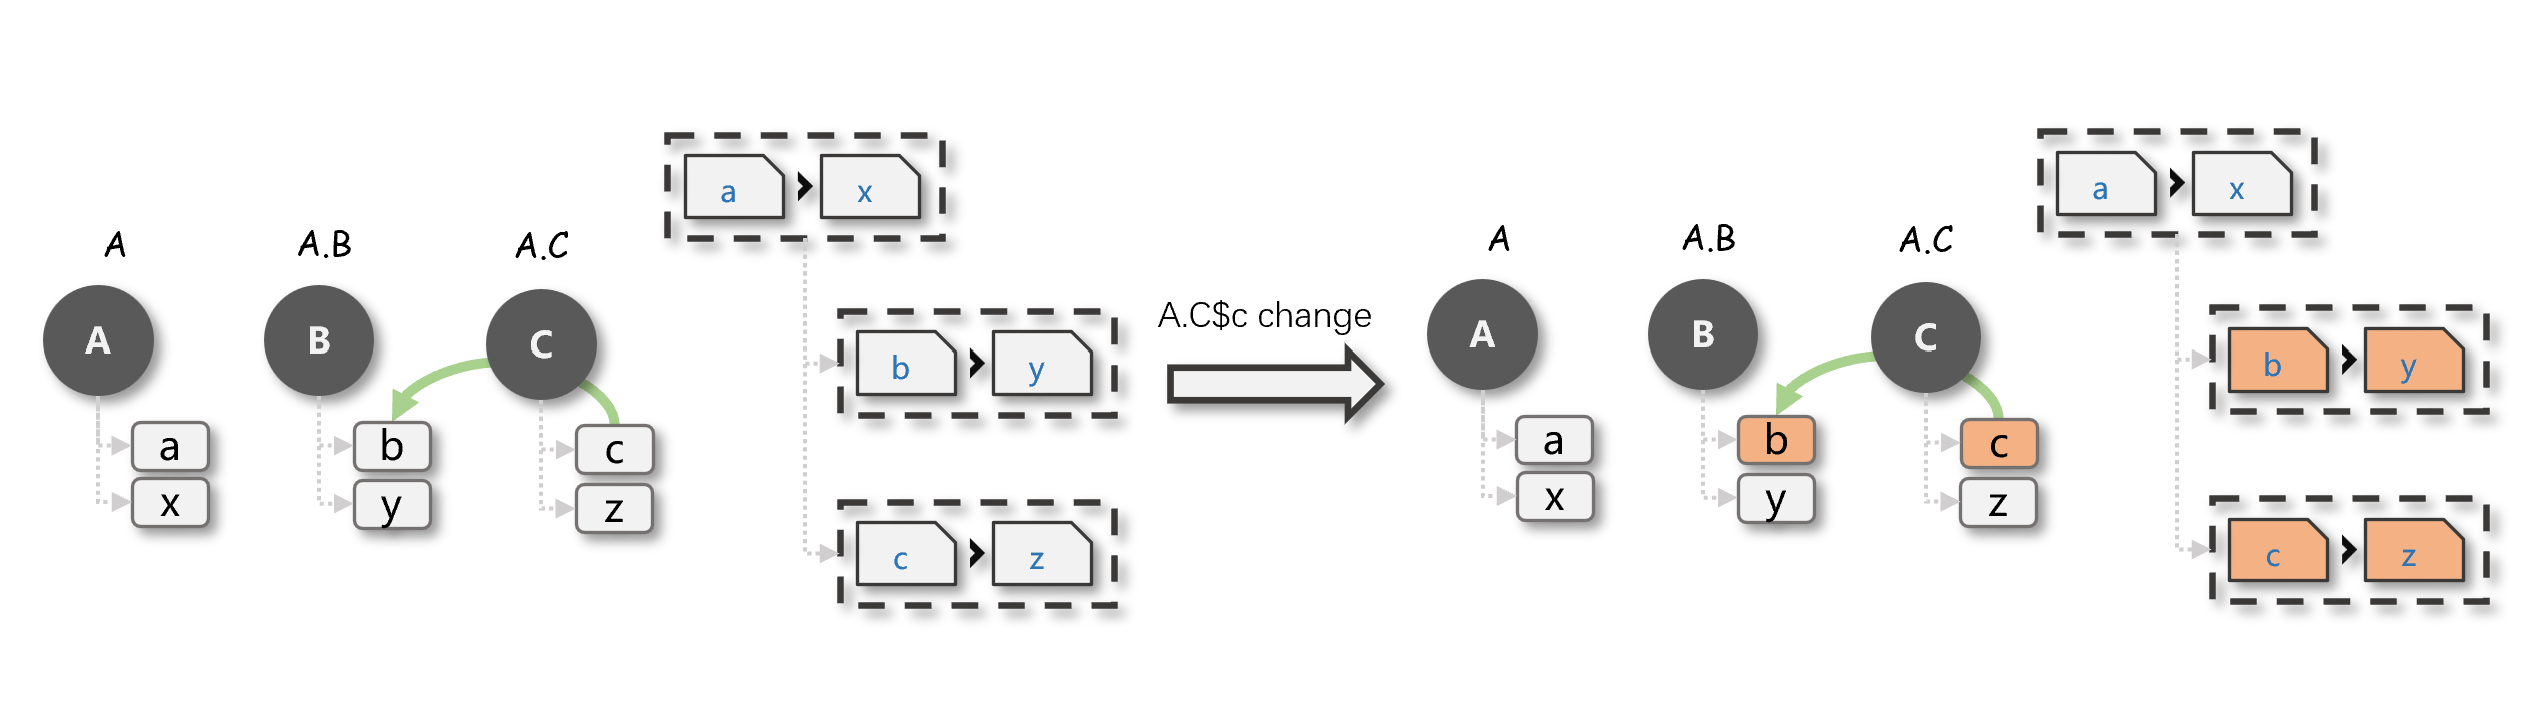
\includegraphics[width=0.9\textwidth]{figure/chapter-2/model-1d.png}
    \caption{模型一维化策略运行效果}
    \label{model-1d}
\end{figure}

以 formily 为代表的一类工具采用的是\textbf{模型一维化}策略(参考\hyperref[model-1d]{图3-4}),其核心思路如下:

\begin{itemize}
    \item 将数据模型中的字段彻底拆分,将其路径作为关键词,以字典的形式组织所有字段,例如:\textbf{上线时间}字段将映射到路径 basicInfo.onlineTime 上。需要强调的是,每个字段仅存储其绑定到复合组件的字段变量,字段之间的父子关系则完全依赖路径进行计算,例如:为了获取\textbf{基础信息}字段的子字段,由于缺少结构信息,只能遍历所有字段的路径,获取前缀为 basicInfo 的字段。
    \item 在此基础上结合订阅-发布模式\footnote{订阅-发布模式是一种消息传递范式,参与消息传递的节点可以在消息总线上订阅特定的消息类型成为 “订阅源”,也可以在消息总线上广播消息成为 “发布源”,最终该消息将由正确匹配的 “订阅源” 捕获以触发预先定义的回调方法,这种模式广泛应用于分布式场景下各类消息中间件的设计中\cite{banavar1999efficient},也常用于 JavaScript 编程过程中涉及到消息传递的场景,例如事件机制\cite{osmani2012learning}},通过 \textit{subscribe} API 实现字段之间的消息订阅,从而实现依赖关系定义,例如:依赖关系 $onlineTime\$errors \rightarrow onlineTime\$value$ 可以定义为:\\$$subscribe(basicInfo.onlineTime\$values, change\ onlineTime\$errors)$$另外,对于更复杂的多字段依赖,formily 还提供了专门的匹配模式语法,例如:依赖关系 $basicInfo\$count \rightarrow (basicInfo's\ all children)\$errors$,可以定义为\footnote{字符 * 表示子字段通配}:\\ $$subscribe(basicInfo.*\$errors,change\ basicInfo\$count)$$
\end{itemize}

在模型一维化策略下,任一字段变量 $Node_x.Attr_y$ 发生变化时,其渲染时间大致可以按照如下方式计算:

\begin{enumerate}
    \item 初始化渲染时间开销 $sum$。
    \item 累加字段 $Node_x$ 对应的复合组件重新渲染的时间 $sum=sum+C*len(CG_x)$。
    \item 遍历 $get\_neighbor(Node_x\$Attr_y)$ 中的字段,重复步骤 2-3。
\end{enumerate}

这种策略实现了\textbf{字段变更仅影响对应的复合组件}的效果,因此性能相较于前三种策略有显著提升,同样考虑\textbf{ID}字段,当用户输入触发 value 变化时,最终的渲染时间约为 $O(C*(len(CG_{ID}))$。

但是 formily 的表单建模方案有一个缺陷,开发人员只能从预设的关键字中选取字段变量进行监听,这就意味着无法实现类似如下形式的依赖关系定义(因为 count 不属于预设关键字):

$$basicInfo\$count \rightarrow (basicInfo's\ all\ children)\$errors$$

此外,由于丢失了结构信息,因此在涉及到子字段操作时,开发人员往往不能直接复用已有的 JavaScript API,例如:\textit{Array} 的 \textit{map} 方法,\textit{Object} 的 \textit{keys} 方法等,重新封装将导致额外的开发代价,这导致模型一维化策略虽然能应对各类规模的数据模型,但是应用场景受限。

而在具体实现时,以模型一维化策略实现的工具例如 formily 的接口设计与全局覆盖策略基本一致,但是由于结构化信息的丢失,该策略引入了重新封装相关 API 的代价,这是不可忽视的。

\section{问题小结}\label{problem-summary}

\subsection{相关工作分析结论}

总的来讲,对现有表单开发方案的渲染性能分析大致有以下结论:

\begin{itemize}
    \item 原生 React:渲染开销取决于依赖关系的复杂程度以及具体实现,无依赖关系的字段通常渲染性能很好,反之较差。
    \item 全局覆盖:渲染开销与数据规模成正比。
    \item 模型切分:渲染开销与深度为 1 的子字段数据规模成正比。
    \item 模型一维化:渲染开销与依赖关系涉及到的字段的变量规模成正比,考虑到实践中字段变量规模通常存在固定的数值范围,因此可以认为是常数级的时间开销。
\end{itemize}

对现有表单开发方案的开发代价大致有以下结论:

\begin{table}[h]
    \centering
    \small
    \begin{tabular}{|l|l|l|l|l|l|}
        \hline
        方案       & 字段定义 & 依赖关系定义 & 复合组件定义 & 组件绑定 & 其他           \\ \hline
        原生 React & 需要     & 需要         & 需要         & 需要     & 区分内外部数据 \\ \hline
        全局覆盖   & 需要     & 需要         & 需要         & 不需要   & 无             \\ \hline
        模型切分   & 需要     & 需要         & 需要         & 不需要   & 无             \\ \hline
        模型一维化 & 需要     & 需要         & 需要         & 不需要   & 应用场景受限   \\ \hline
    \end{tabular}
    \normalsize
    \caption{表单开发方案的开发代价总结}
\end{table}

通过几个方案的对比本文得出一个重要结论:数据更新的粒度越细,触发重新渲染的组件数量越少,渲染性能就越好。
理论上任一变量变更时,如果能够仅重新渲染该变量对应的基础组件以及更新其依赖关系对应的变量,就能达成最优的渲染性能。

结合上文提出的建模方法来表述,通过只对任意变量基于依赖关系和映射关系得到的最小变量和基础组件闭包进行更新,就可以达成理论上的最优性能,本文将之称为\textbf{精准更新}策略。

响应式编程方法是解决依赖关系(变量与组件的映射关系也同理)定义的一个常用策略\cite{bainomugisha2013survey},其核心思路是监听参与运算的变量,在变量发生变化时,重新计算与之存在依赖关系的所有变量,实现任意数据的依赖关系精准触发。分别在数据模型和组件渲染层面分别应用响应式编程方法,就能实现精准更新策略,进而大幅提高渲染性能。具体来讲:

\begin{itemize}
    \item 数据模型层面需要实现依赖关系的响应式触发,即任意变量变化时,只更新与之存在依赖关系的变量。
    \item 组件渲染层面需要实现基础组件的响应式渲染,例如:$id\$value$ 变化时,只对基础组件 Input 进行重新渲染。
\end{itemize}

此外,通过对模型一维化策略的分析,本文得出结论:针对\textbf{多字段依赖定义},路径机制可以结合特定的匹配模式语法很好地处理该问题,但是破坏逻辑存储结构可能会极大地增加后续地开发代价,因此一个更好的实现方式应该是在保持逻辑存储结构的前提下实现多字段依赖定义,而这一实现可以在数据模型层面进行。此外,预设关键字进行模型管理的方案会限制开发场景,为了实现需求场景的全面覆盖,应当提供任意变量的变化都可以进行监听的机制。

\subsection{解决方案}\label{final-solution}

本文将分别从数据模型设计和组件渲染适配两个维度设计方案来实现上文提出的几个目标(以下将该解决方案简称为 XForm 方案)。

首先在数据模型设计层面,本文将应用观察者模式\footnote{观察者模式是一种基于对象变更监听实现依赖关系管理的设计模式\cite{gamma1995design}}构建一个响应式数据模型,从根本上提升性能,在此基础上,为了实现多字段依赖管理,本文参考 formily 的实现方案,在保留模型逻辑存储结构的前提下实现数据模型的路径管理。

其次在框架适配方面,本文将使用一套框架特定的组件渲染流程替换 React 框架原生的基于 state 变更触发 VDOM diff 操作的流程,以实现响应式渲染的效果。此外,为了使组件能够适配数据模型的路径系统,本文引入了\textbf{模型分发}机制以实现路径上下文的维护。在具体功能上,需要提供字段定义,变量定义、依赖关系定义的接口,以及基础组件的声明式定义接口,以应对表单场景的各类需求。

\begin{figure}[h]
    \centering
    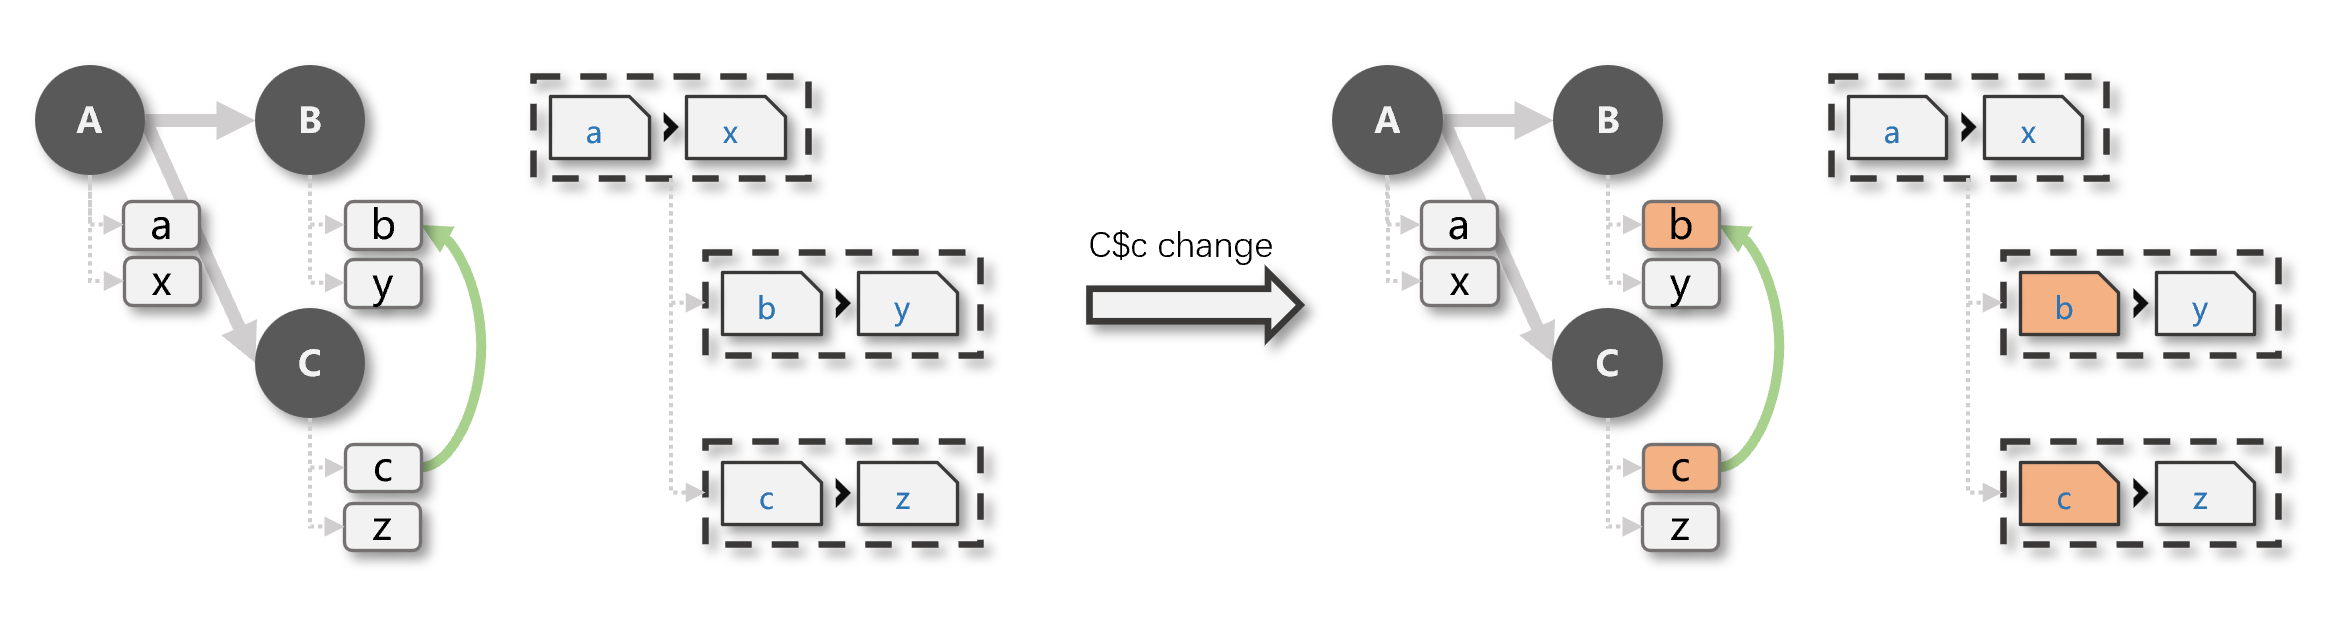
\includegraphics[width=0.9\textwidth]{figure/chapter-2/accurate.png}
    \caption{XForm 方案理论运行效果}
    \label{accurate}
\end{figure}

这套方案的理论渲染性能大致可以建模为如下形式(参考\hyperref[accurate]{图3-5}):

\begin{itemize}
    \item 设边权重 $w(Dep_t)$ 为对应依赖关系的计算开销。
    \item $edge\_closure(Node_x\$Attr_y)$ 为任一字段变量 $Node_x\$Attr_y$ 的依赖关系组成的字段变量闭包,形式上是一组字段变量的集合。
    \item 相应地,$node\_closure(Node_x\$Attr_y)$ 为任一字段变量经由依赖关系连接的节点闭包。
    \item $len(xxx\_closure)$ 用于表示某闭包内元素的个数。
\end{itemize}

最终,单个变量$Node_x\$Attr_y$变更时,渲染的时间开销满足如下公式:

\begin{equation}
O(len(node\_closure(Node_x\$Attr_y)*C)+\sum_{Dep_t\in edge\_closure(Node_i)}w(Dep_t))
\end{equation}

考虑大规模数据模型场景下的渲染性能,相较于全局覆盖策略和模型切分策略,XForm 方案大致可以达成 $O(n)\rightarrow O(1)$ 的提升,其中 $n$ 表示数据模型字段变量总数,相较于模型一维化策略大致为 $O(k)\rightarrow O(1)$ 的提升,其中 $k$ 表示数据模型单个字段的变量总数。

同时 XForm 方案通过简化接口降低了开发代价,并且覆盖了现有工具的功能场景。

这些提升效果将在\hyperref[experiment-examine]{第五章}中进一步通过实验验证。

\chapter{基于路径的响应式数据模型管理}\label{reactive-datamodel-based-on-path-system}

为了实现数据的响应式更新和多字段依赖定义,本文将数据模型的实现方案拆解为以下三个部分:

\begin{itemize}
    \item \textbf{响应式数据模型}:部分相关工作采用覆盖式更新策略的一个重要原因在于,它可以比较简单地实现依赖关系的管理,将大部分计算工作交由渲染框架进行,这也是其性能瓶颈的根源。\\ 依赖关系的本质是某个数据变更触发其他的数据变更,因此如果能够精准地监听目标数据的变更,并相应地触发依赖数据的变更,而不影响其他无关数据,无疑能够大幅降低计算开销。\\ 恰好 JavaScript 标准提供了精准拦截数据操作方法的 Proxy 类,因此通过合理的算法设计完全可以实现依赖精准触发的目标。
    \item \textbf{路径系统}:由于依赖精准触发机制没有对 JavaScript 对象进行侵入性的更改,因此数据模型的逻辑结构天然地实现了维护,但是为了实现对数据模型的每个字段精准快速地访问,还需要结合路径系统,为每个字段维护其路径关键字,以便于后续进行多字段依赖关系的管理。
    \item \textbf{多字段依赖管理}:基于路径系统,开发者可以通过枚举依赖项实现多字段依赖关系定义,但是这种方式无法实现路径通配、路径反向匹配、范围匹配等语义,因此,对于涉及变量个数较多的依赖关系,枚举的方式不仅需要额外书写大量代码,还会导致回调方法的冗余注册。为了提供更便捷的多字段依赖关系定义机制,本文引入了路径匹配语法以及消息总线机制,从而大幅简化多字段依赖定义的方式。
\end{itemize}

\section{响应式数据模型}

为了实现数据更新时精准触发依赖关系的目标,本文设计了一套基于 JavaScript 对象代理机制实现依赖关系的自动收集和触发的算法,并针对全属性依赖、上下文无关依赖等边界情况作了进一步的算法优化,通过该算法封装的对象统称为响应式数据模型。

\subsection{JavaScript Proxy}

\textit{Proxy} 是 JavaScript 的一个内置类,用于创建 JavaScript 对象的代理,从而实现基本访问操作的拦截和重写,\textit{Proxy}类创建对象代理实例的样例代码如下:

\lstinputlisting[style=proxy-example,caption={创建 JavaScript 对象代理},captionpos=b]{code/chapter-3/proxy.js}

通过上述样例代码创建的对象代理,其表现与一般的 JavaScript 对象几乎一致,唯一的区别在于,在触发特定的访问操作时,会执行经过重写的方法,例如语句 \textit{const x = proxyObject.a} 会触发重写的 \textit{get} 方法,语句 \textit{proxyObject.a = 10} 会触发重写的 \textit{set} 方法。

\subsection{依赖收集算法 1.0}

\begin{figure}[h]
    \centering
    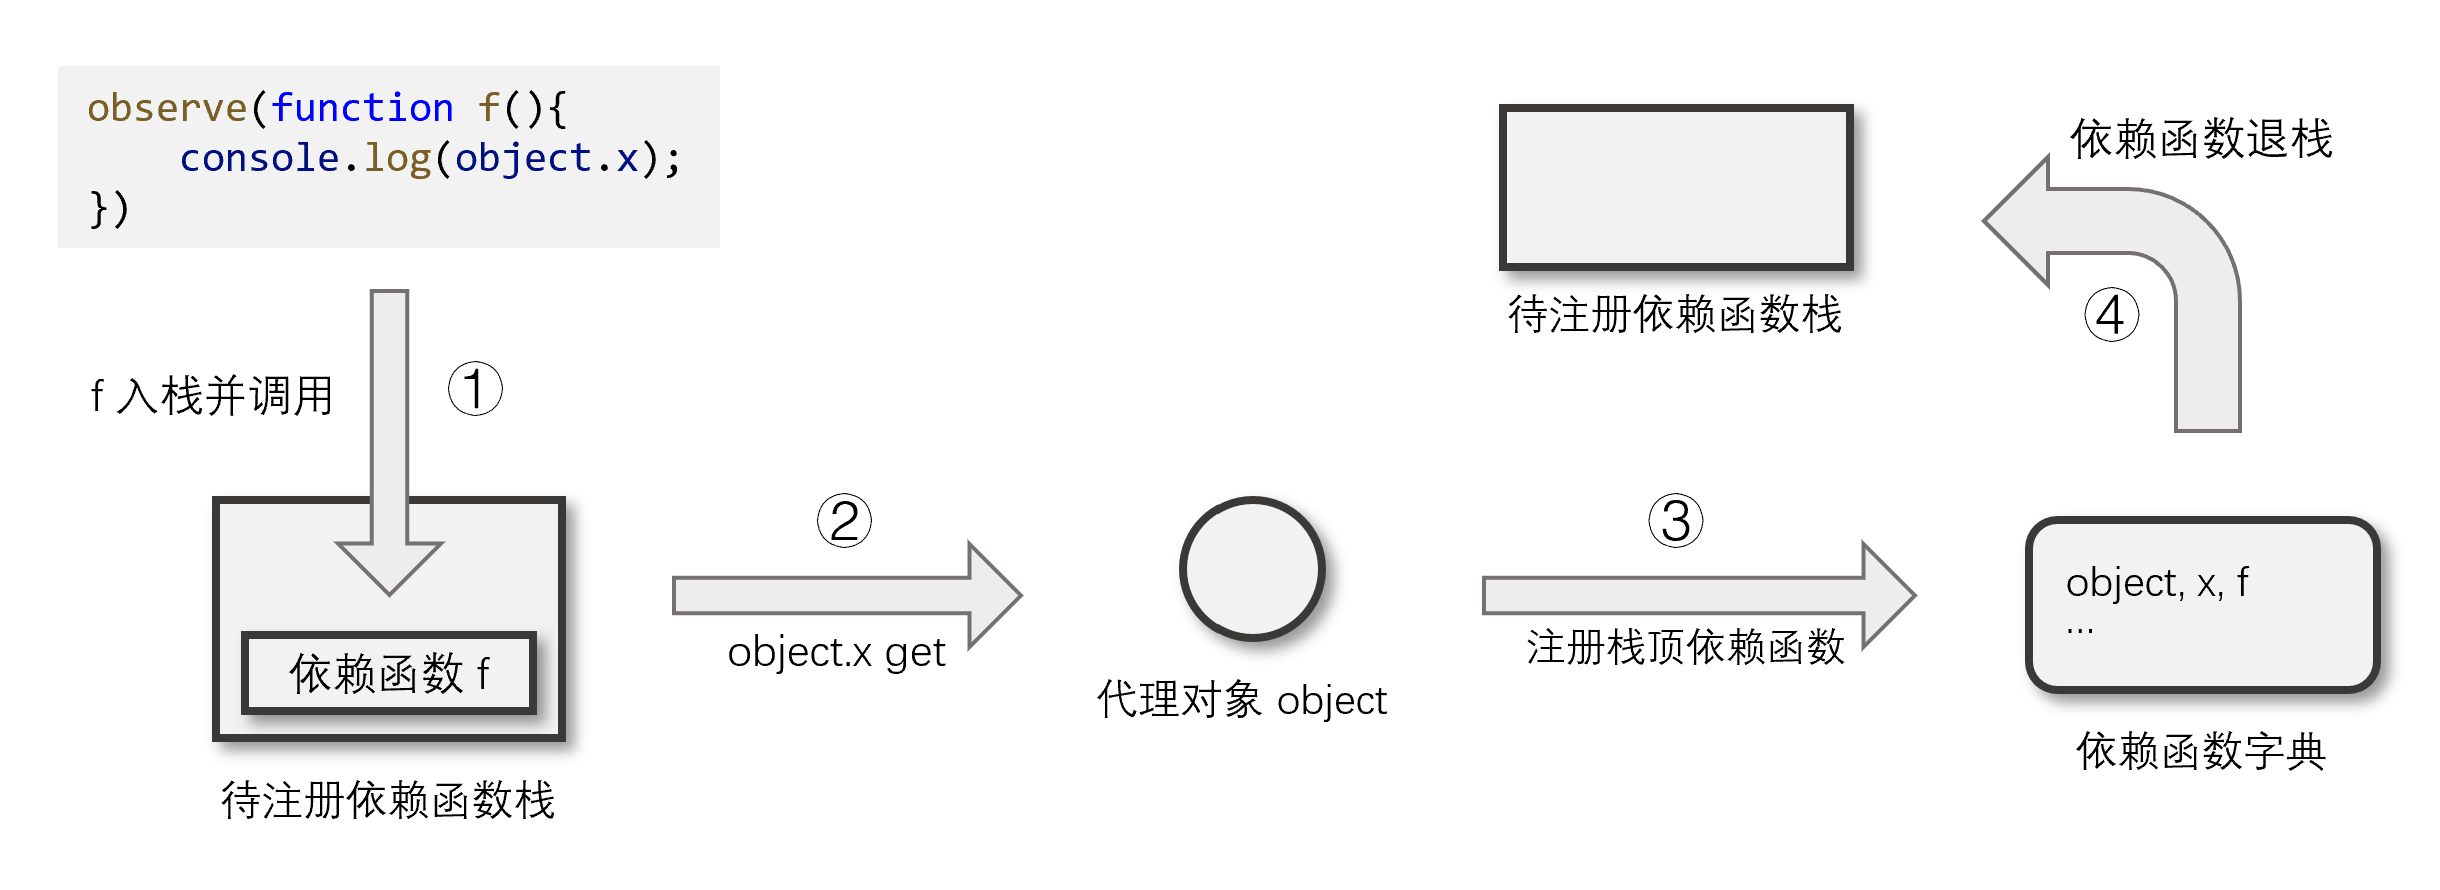
\includegraphics[width=\textwidth]{figure/chapter-3/algorithm1.0-update.png}
    \caption{依赖收集算法1.0}
    \label{algorithm-1.0}
\end{figure}

假设存在某函数,其执行过程对目标对象特定属性的关键字进行了 \textit{get} 操作,并且需要在相应属性变更时自动地触发该函数,则将该函数称作\textbf{依赖函数(dependency function)},通过使用 \textit{Proxy} 进行对象代理,结合如下算法,就可以为相关属性将该函数注册为回调方法,进而在属性变更时,自动地触发相应的依赖函数。

实现依赖函数注册的算法为\hyperref[dependency-collect-algorithm-1.0]{依赖收集算法1.0},具体流程大致如\hyperref[algorithm-1.0]{图4-1} 所示。

\begin{algorithm}[H]
    \caption{依赖收集算法 1.0}
    \label{dependency-collect-algorithm-1.0}
    \begin{algorithmic}[1]
        \REQUIRE 待注册的依赖函数 \textit{func} : Function
        \STATE $\text{cbMap} \gets \text{Map}\langle \text{Object}, \text{Map}\langle \text{String}, \text{Function}[]\rangle\rangle$ \footnotesize\textcolor{gray}{// [对象,关键字,函数列表]的字典}\normalsize
        \STATE $\text{cbStack} \gets \text{Function}[]$ \footnotesize\textcolor{gray}{// 依赖函数运行时的调用栈}\normalsize
        \STATE $\text{cbStack}.push(\textit{func})$,调用 \textit{func}
        \WHILE {\textit{func} 运行中}
        \IF{ 对象 $objectA$ 的 $key\_a$ 属性的 \textit{get} 方法被触发}
        \IF{ $\text{cbStack}$ 不为空}
        \STATE $\text{cbMap}[objectA][key\_a].push(\textit{cbStack.top()})$
        \ENDIF
        \ENDIF
        \ENDWHILE
        \STATE $\text{cbStack}.pop()$
    \end{algorithmic}
\end{algorithm}

通过上述算法完成依赖函数的注册后,当目标对象发生赋值操作 \textit{objectA.key\_a = someValue} 触发 \textit{set} 方法时,就可以通过查找字典获取对应的依赖函数列表并逐个触发。大部分 JavaScript 类的实例对象都适用于该算法,但由于部分类的特定方法存在副作用,因此在具体的代码实现中,依然有一些边界情况需要特殊处理。

\subsection{全属性依赖:依赖收集算法 1.1}

\begin{figure}[h]
    \centering
    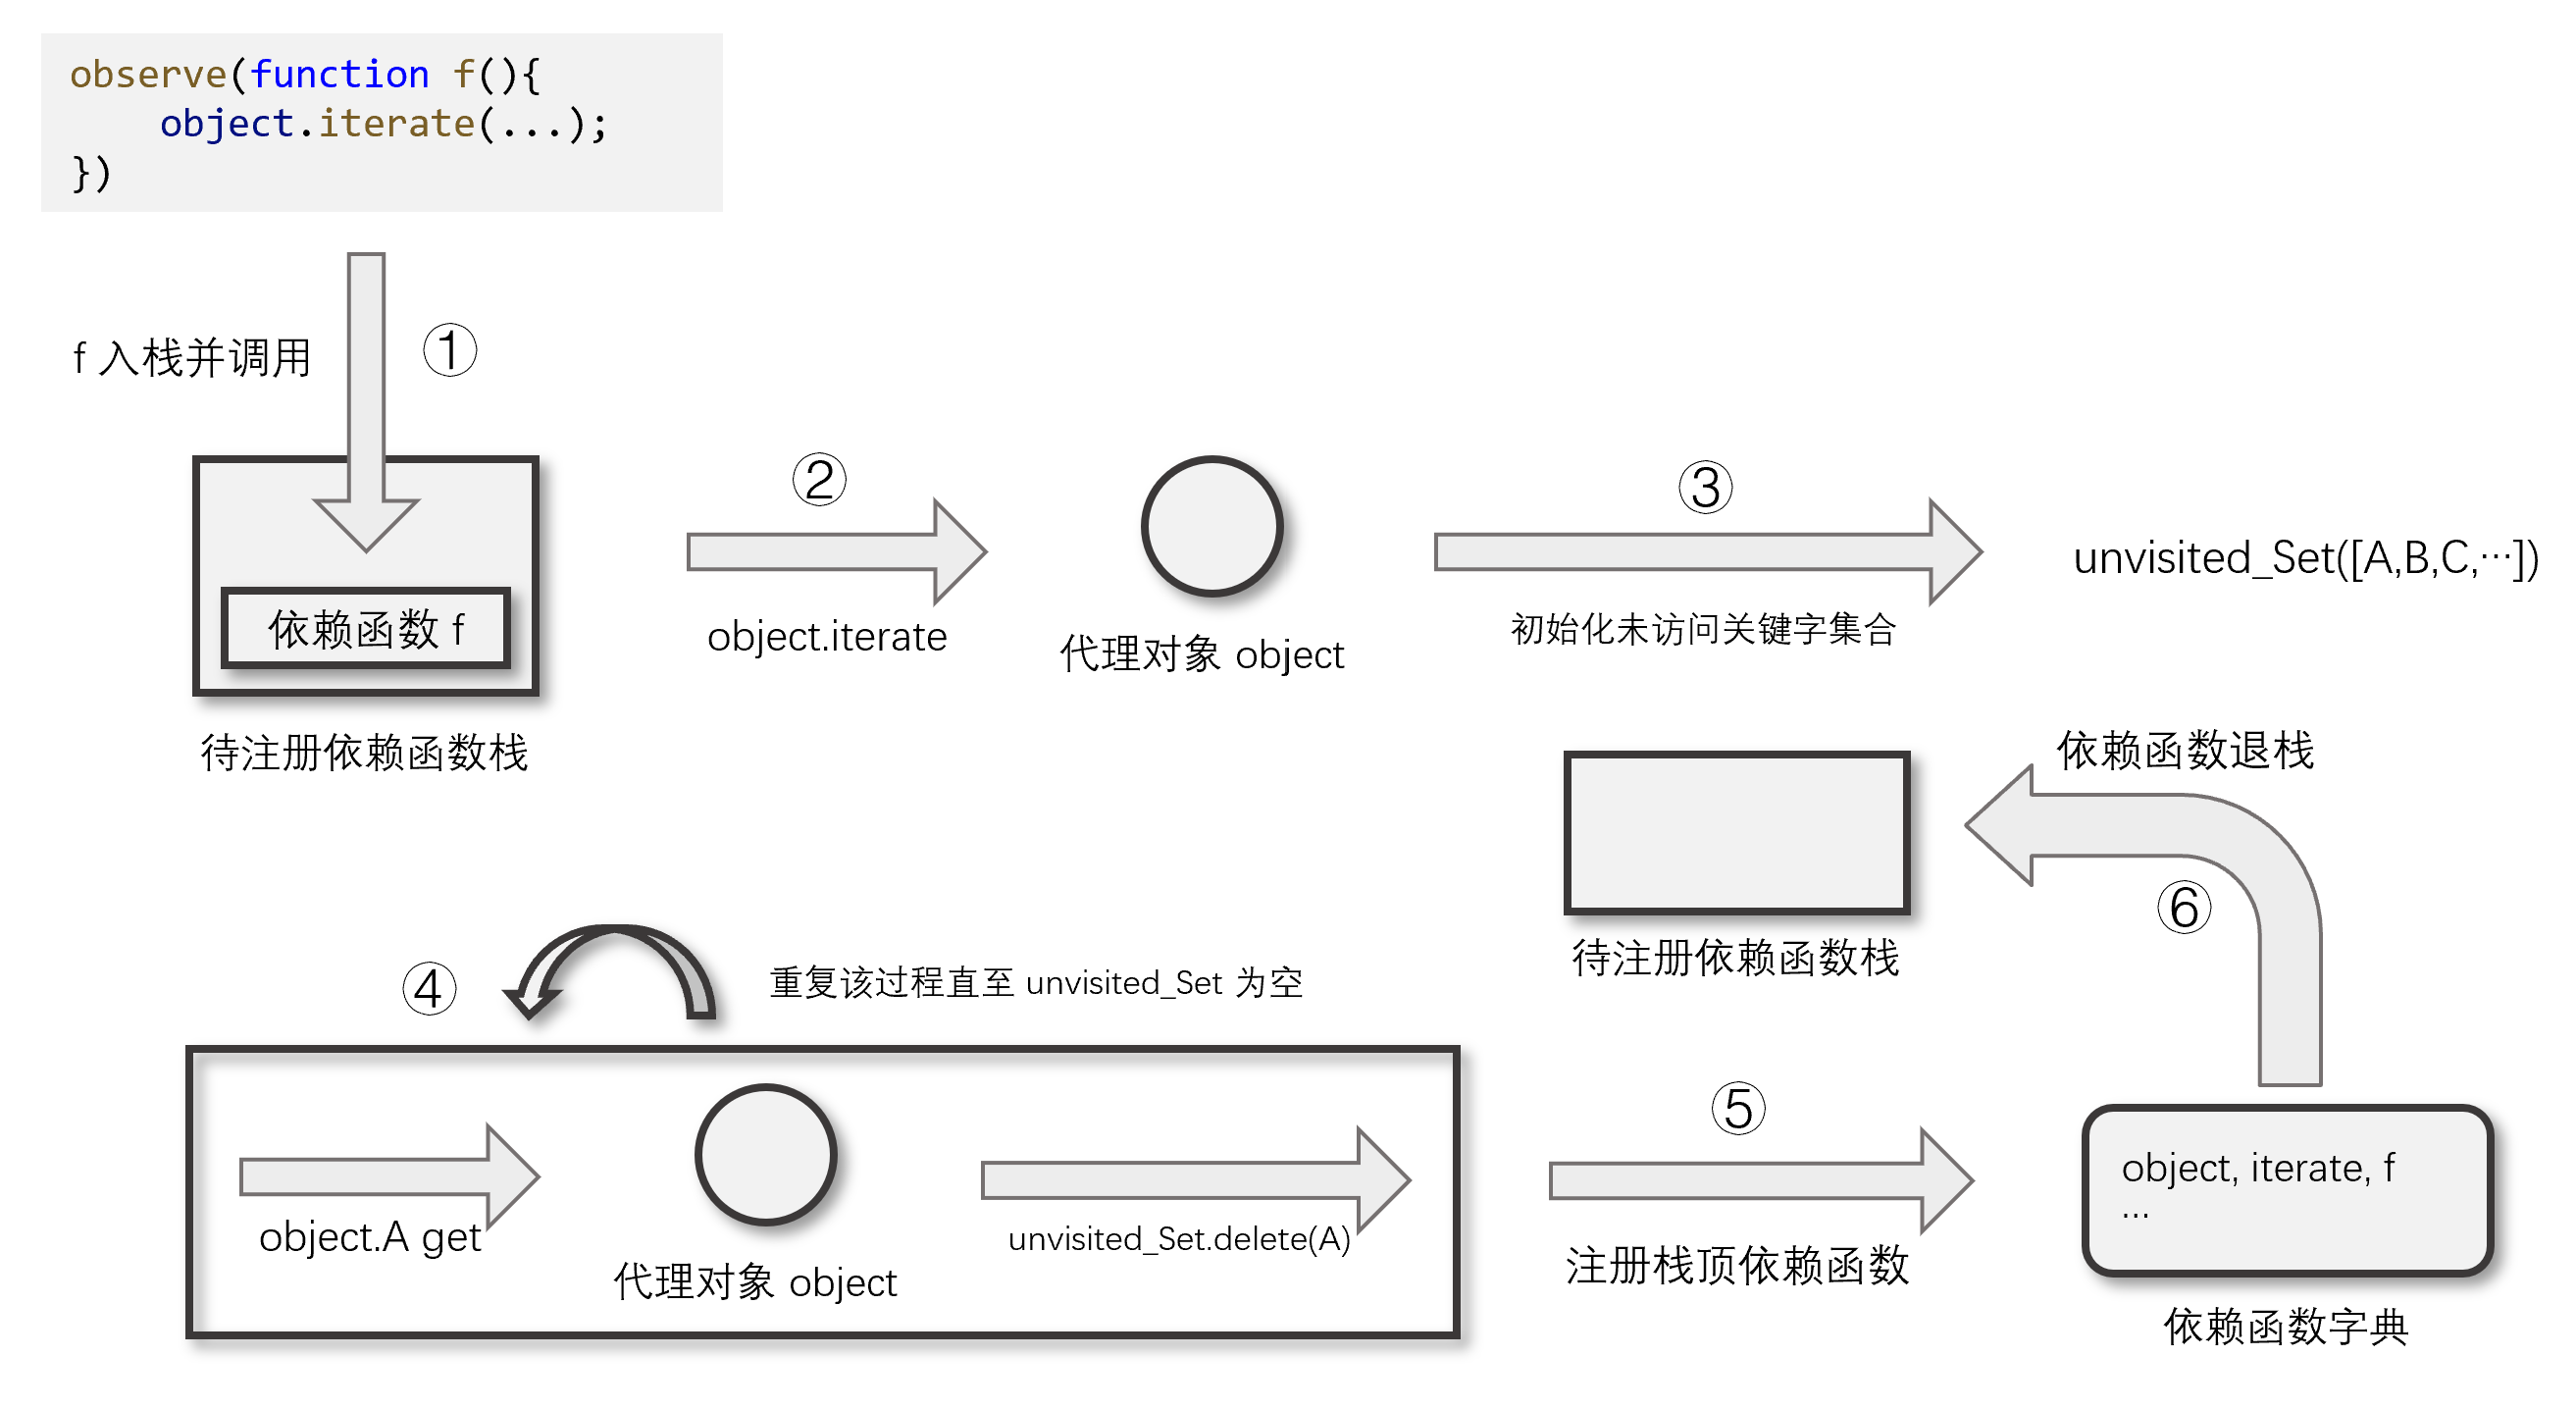
\includegraphics[width=\textwidth]{figure/chapter-3/algorithm1.1-update.png}
    \caption{依赖收集算法1.1}
    \label{algorithm-1.1}
\end{figure}

属性遍历是 JavaScript 开发过程中常见的操作,即部分依赖函数可能会遍历目标对象的所有属性,其语义大致为:目标对象的任意属性发生变更时,都触发一次对应的依赖函数,简称为\textbf{全属性依赖函数}。

对于基础的对象类型,全属性依赖函数可以通过简单地重写 \textit{ownKeys} 方法\footnote{JavaScript 针对目标对象关键字的遍历操作提供的 API,可以应对大部分遍历操作的开发场景}
并结合特殊属性关键字 \textit{iterate} 来实现,但是如数组类型 \textit{Array} 的特殊对象,在调用特定的 API 时会逐个触发所有索引 \textit{[0, 1, 2, \dots]} 的 \textit{get} 方法,这就导致了两个问题:

\begin{enumerate}
    \item 回调方法在 \textit{iterate} 和其他索引上重复注册,当数组项发生变更时,同一回调方法会分别执行两次,形成冗余,与全属性依赖函数的语义不一致。
    \item 当数组插入新的值时,由于回调方法已经完成注册,因此不会在新的索引上重复注册,则这部分新的数组值在变更时,回调方法仅会执行一次,这导致新旧数据的行为出现了不一致。
\end{enumerate}

为了解决这个问题,本文在\hyperref[dependency-collect-algorithm-1.0]{依赖收集算法 1.0} 的基础上给出了针对全属性依赖函数语义的变种设计\hyperref[dependency-collect-algorithm-1.1]{依赖收集算法 1.1},具体流程如\hyperref[algorithm-1.1]{图4-2} 所示。

\begin{algorithm}[H]
    \caption{依赖收集算法 1.1}
    \label{dependency-collect-algorithm-1.1}
    \begin{algorithmic}[1]
        \REQUIRE 待注册的依赖函数 \textit{func} : Function
        \STATE $\text{cbMap} \gets \text{Map}\langle \text{Object}, \text{Map}\langle \text{String}, \text{Function}[]\rangle\rangle$ \footnotesize\textcolor{gray}{// [对象,关键字,函数列表]的字典}\normalsize
        \STATE $\text{cbStack} \gets \text{Function}[]$ \footnotesize\textcolor{gray}{// 依赖函数运行时的调用栈}\normalsize
        \STATE $\text{unvisitedKeySet} \gets \text{Set}\langle\text{String}\rangle$\footnotesize\textcolor{gray}{// 未访问的关键字集合}\normalsize
        \STATE $\text{cbStack}.push(\textit{func})$,调用 \textit{func}
        \WHILE {\textit{func} 运行中}
        \IF{对象 $objectA$ 的 $method\_a$ 属性的 \textit{get} 方法被触发 \\~~~~\textbf{and} $objectA[method\_a]$ 为函数类型 \\~~~~\textbf{and} $objectA[method\_a]$ 执行过程包含遍历操作}
        \STATE $\text{unvisitedKeySet} \gets \text{Set}(All\ keys\ of\ objectA)$
        \ENDIF
        \IF{ 对象 $objectA$ 的 $key\_a$ 属性的 \textit{get} 方法被触发}
        \IF{ $\text{unvisitedKeySet}$ 不为空}
        \STATE $\text{unvisitedKeySet}.delete(key\_a)$
        \ENDIF
        \IF{ $\text{cbStack}$ 不为空 \textbf{and} $\text{unvisitedKeySet}$ 为空}
        \STATE $\text{cbMap}[objectA][key\_a].push(\textit{cbStack.top()})$
        \ENDIF
        \ENDIF
        \ENDWHILE
        \STATE $\text{cbStack}.pop()$
    \end{algorithmic}
\end{algorithm}

\subsection{上下文无关依赖:依赖收集算法 1.2}\label{reactive-data-model-context-free-dependency}

基于算法\hyperref[dependency-collect-algorithm-1.1]{依赖收集算法 1.1},一个完整的响应式数据模型可以通过结合对象代理以及相应的依赖函数定义来表达了,例如:依赖关系 $A.a \rightarrow A.b$ 可以通过\hyperref[create-reactive-data-model]{代码4.2} 的方式定义。

但是使用这种方式,依赖函数的定义是严格依赖于对象代理的上下文的,因此通常情况下,不能直接复用局部的模型设计,例如将样例模型作为子模型嵌套地定义到另一个模型中时,需要相应地更改依赖函数的实现才能正确地迁移依赖关系,如\hyperref[reuse-reactive-data-model]{代码4.3} 所示。

随着模型规模扩大,其修改代价也会随之增加,对于上下文无关的依赖关系,这种修改代价降低了代码的可维护性,显然是不必要的,因此本文设计了\hyperref[dependency-collect-algorithm-1.2]{依赖收集算法 1.2} 针对此类依赖关系的定义给出了进一步的优化。

基于\hyperref[dependency-collect-algorithm-1.2]{依赖收集算法 1.2},上下文无关的依赖关系就可以直接在模型定义时声明,并且不需要修改依赖关系的定义就可以直接迁移到其他模型内部,从而提高代码的可复用性,如\hyperref[reuse-reactive-data-model-without-modify]{代码4.4} 所示。

\begin{algorithm}[H]
    \caption{依赖收集算法 1.2}
    \label{dependency-collect-algorithm-1.2}
    \begin{algorithmic}[1]
        \REQUIRE 待注册的依赖函数 \textit{func} : Function
        \STATE $\text{cbMap} \gets \text{Map}\langle \text{Object}, \text{Map}\langle \text{String}, \text{Function}[]\rangle\rangle$ \footnotesize\textcolor{gray}{// [对象,关键字,函数列表]的字典}\normalsize
        \STATE $\text{cbStack} \gets \text{Function}[]$ \footnotesize\textcolor{gray}{// 依赖函数运行时的调用栈}\normalsize
        \STATE $\text{unvisitedKeySet} \gets \text{Set}\langle\text{String}\rangle$\footnotesize\textcolor{gray}{// 未访问的关键字集合}\normalsize
        \STATE $\text{cbStack}.push(\textit{func})$,调用 \textit{func}
        \WHILE {\textit{func} 运行中}
        \IF{对象 $objectA$ 的 $method\_a$ 属性的 \textit{get} 方法被触发 \\~~~~\textbf{and} $objectA[method\_a]$ 为函数类型}
        \IF{$objectA[method\_a]$ 执行过程包含遍历操作}
        \STATE $\text{unvisitedKeySet} \gets \text{Set}(All\ keys\ of\ objectA)$
        \ELSIF{$objectA[method\_a]$ 为依赖函数}
        \STATE 对 $objectA[method\_a]$ 递归执行算法\ref{dependency-collect-algorithm-1.2}
        \ENDIF
        \ENDIF
        \IF{ 对象 $objectA$ 的 $key\_a$ 属性的 \textit{get} 方法被触发}
        \IF{ $\text{unvisitedKeySet}$ 不为空}
        \STATE $\text{unvisitedKeySet}.delete(key\_a)$
        \ENDIF
        \IF{ $\text{cbStack}$ 不为空 \textbf{and} $\text{unvisitedKeySet}$ 为空}
        \STATE $\text{cbMap}[objectA][key\_a].push(\textit{cbStack.top()})$
        \ENDIF
        \ENDIF
        \ENDWHILE
        \STATE $\text{cbStack}.pop()$
    \end{algorithmic}
\end{algorithm}

\hyperref[dependency-collect-algorithm-1.2]{依赖收集算法 1.2} 保证了响应式数据模型的基本功能,本文在具体的实现中将响应式输入模型抽象成了工厂类 \textbf{ReactiveFactory},其核心 API 包括

\begin{itemize}
    \item \textbf{ReactiveFactory}:用于管理一组存在依赖关系的响应式数据模型的工厂类,考虑到同一页面内可能存在独立的多组响应式数据模型,因此实现了该工厂类用于实现它们的隔离。
    \item \textbf{ReactiveFactory.reactive}:将目标对象封装为响应式的对象。
    \item \textbf{ReactiveFactory.observe}:将目标函数注册为依赖函数。
\end{itemize}

\begin{center}
    \begin{minipage}{0.3\textwidth}
        \lstinputlisting[label={create-reactive-data-model},style=proxy-example,caption={依赖定义},captionpos=b]{code/chapter-3/model.js}
    \end{minipage}\quad
    \begin{minipage}{0.3\textwidth}
        \lstinputlisting[label={reuse-reactive-data-model},style=proxy-example,caption={修改定义复用},captionpos=b]{code/chapter-3/submodel.js}
    \end{minipage}\quad
    \begin{minipage}{0.3\textwidth}
        \lstinputlisting[label={reuse-reactive-data-model-without-modify},style=proxy-example,caption={直接复用},captionpos=b]{code/chapter-3/innersubmodel.js}
    \end{minipage}
\end{center}

\textit{注:下文若无特殊说明,将省略 ReactiveFactory,直接使用 reactive 和 observe 方法进行样例讲解。}

\section{路径系统}

为了充分支持并利用表单数据模型的树结构特性,本文在响应式数据模型的基础上给出了一种路径系统的设计方案,表单数据模型中的字段按照其管理的数据类型大致可以分为三类:

\begin{enumerate}
    \item \textbf{基本数据字段(Field)}:模型设计树结构上的叶子节点,无需提供子节点的增删逻辑,通常用来管理 String、Number、Boolean 等类型的 JSON 数据\footnote{实际上,只要不涉及到依赖关系定义,基本数据字段可以管理更复杂的 JavaScript 对象,为便于理解此处仅以基本类型为例}
    \item \textbf{对象数据字段(ObjectField)}:与 JSON 的 Object 类型对应,用于管理以字符串为关键字的子字段
    \item \textbf{数组数据字段(ArrayField)}:与 JSON 的 Array 类型对应,用于管理以数字索引为关键字的子字段
\end{enumerate}

其 JavaScript 代码实现为三个对应的类,基于这三个类,以前文所述的考拉海购表单为例,其部分表单模型可以通过如下代码初始化\footnote{路径系统的类已经针对响应式数据模型进行了适配,原生地支持自动依赖收集和精准触发}:

\lstinputlisting[label={kaola-model-definition-code},style=proxy-example,caption={基于路径系统的考拉海购案例表单模型声明(不含依赖关系)},captionpos=b]{code/chapter-3/kaola-field-intialize.js}

通过还原模型的树结构,实际上从根节点出发到任意字段的路径已经天然地形成了字段的关键字,例如\textit{ID} 字段的路径关键字为 \textit{SiteConfiguration.BasicInfo.ID},从而可以通过路径管理所有字段,具体来讲,本文设计的路径系统提供了一系列 API 分别用于完成字段的创建、查找、删除、更新、以及多字段依赖关系管理等操作。

基于响应式数据模型和路径系统,多字段依赖已经可以直接通过定义依赖函数来解决了,但美中不足的是,这种依赖关系定义方式的可读性较差,缺少一种直观的表达方式;同时,在声明 “一对多依赖” 时,同一个依赖函数需要重复注册到所有对应的字段上,某种程度上造成了资源的浪费\footnote{除了重复注册依赖函数的时间开销之外,保存依赖函数的映射关系也需要额外的空间开销},因此本文采取了进一步的解决方案来实现多字段依赖管理。

\section{多字段依赖定义}

本文对多字段依赖定义的实现方案分为两个方面:首先,要实现多字段依赖定义需要对应的描述语法;其次,要实现一套可用的管理机制来完成依赖关系的注册和调用。

\subsection{字段路径匹配}\label{node-path-match}

多字段依赖定义可以基于路径系统抽象成一组路径对应的字段与单个路径对应的字段之间\footnote{更精确地讲,是字段的变量之间}的关系,一般地,可以使用正则表达式来描述一组路径,例如通过如下方式描述依赖 $A.a \rightarrow \text{Set}([All\ of\ B's\ direct\ children's\ x\ variable])$:

\lstinputlisting[style=proxy-example,caption={使用正则表达式描述一组路径},captionpos=b]{code/chapter-3/re.js}

在实践中,路径集合大致需要通配、反向匹配、范围匹配等描述能力,正则表达式可以很好地覆盖此类语义,但是较低的抽象层次也导致其代码的可读性较差,因此,为了更好地结合表单模型树结构的特性,本文给出了一种针对路径系统的模式匹配语法设计,文法大致如下:

\lstinputlisting[style=proxy-example,caption={路径匹配模式文法(Path Match Pattern Grammar)},captionpos=b]{code/chapter-3/match-pattern.txt}

上述文法使用递归下降算法\cite{burge1975recursive}实现,以下样例代码选自部分测试用例:

\lstinputlisting[style=proxy-example,caption={路径匹配模式样例},captionpos=b]{code/chapter-3/match-pattern-example.txt}

除了提供上述匹配模式语法以描述路径集合之外,考虑到表单数据模型也需要上下文无关的表达能力(参考 \hyperref[reactive-data-model-context-free-dependency]{4.1.4节}的讨论),本文还提供了回溯路径语法用于进行路径拼接以实现上下文无关的路径访问,其文法如下:

\lstinputlisting[style=proxy-example,caption={路径回溯模式文法(Path Backtrack Pattern Grammar)},captionpos=b]{code/backtrack-pattern.txt}

路径回溯模式样例代码如下:

\lstinputlisting[style=proxy-example,caption={路径回溯模式样例},captionpos=b]{code/backtrack-pattern-example.txt}

\subsection{消息总线}

\begin{figure}[h]
    \centering
    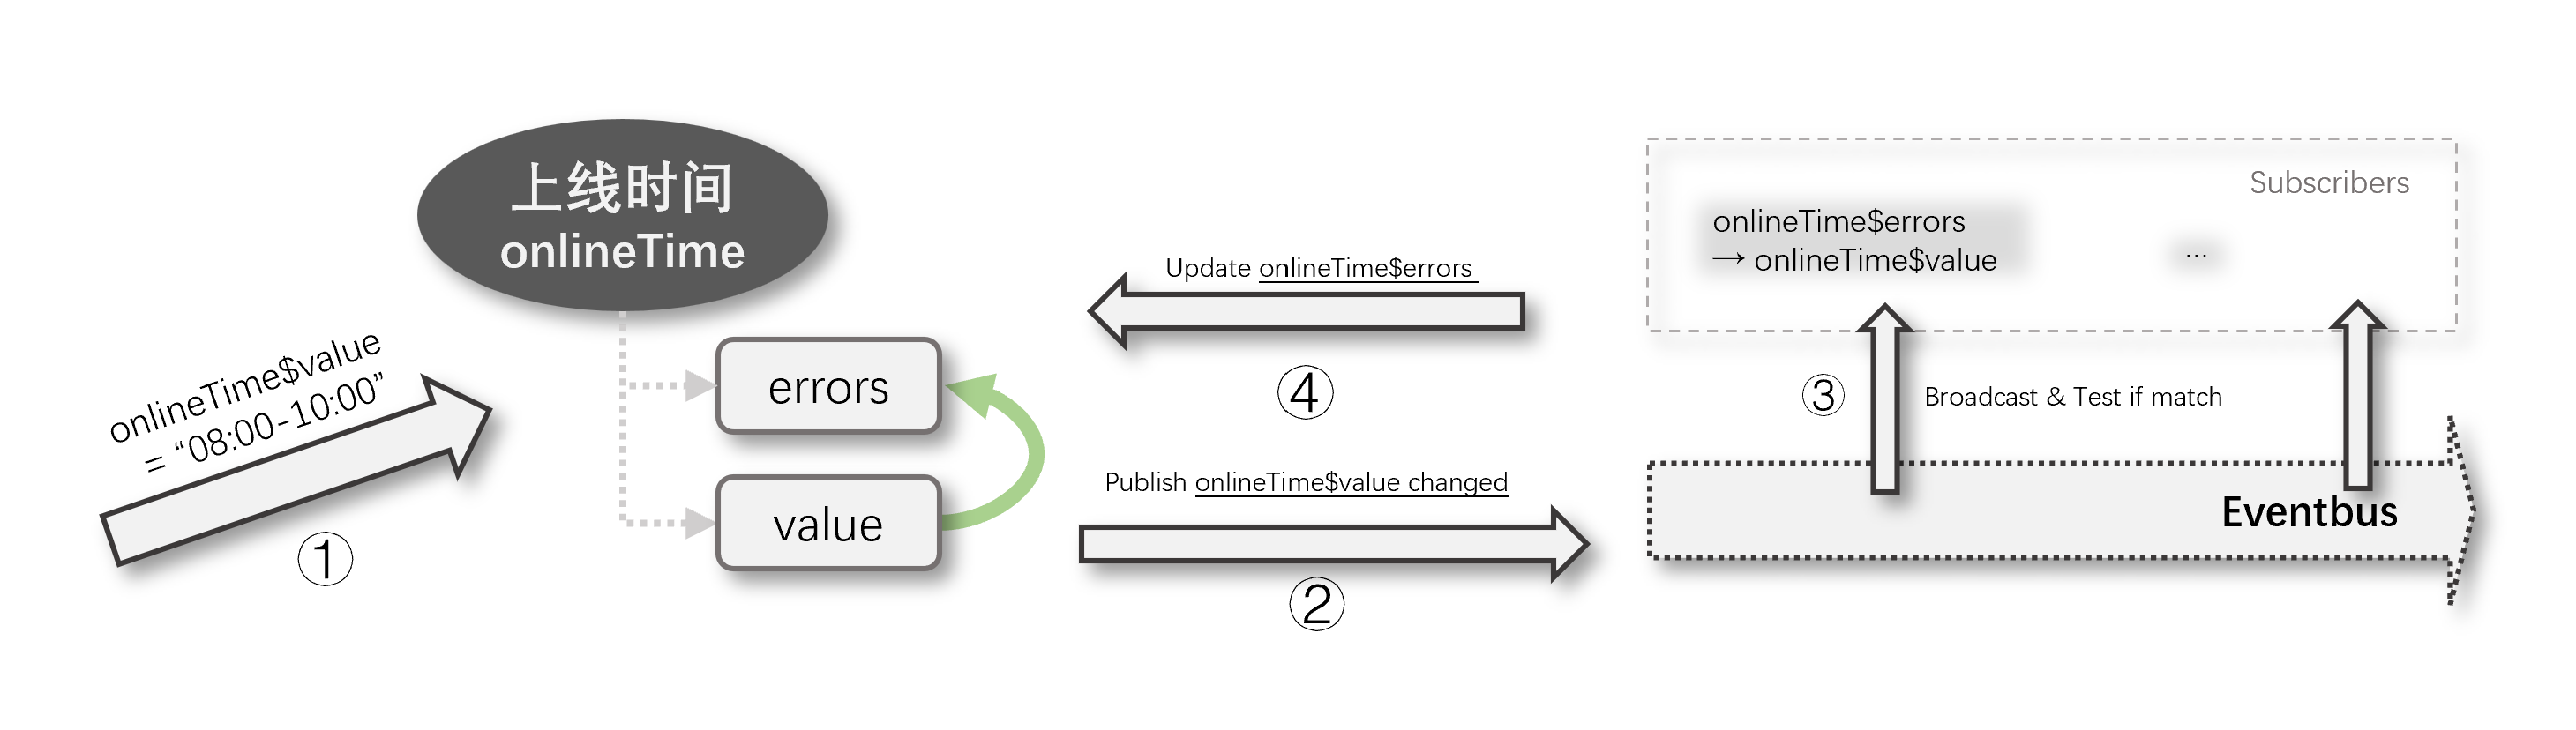
\includegraphics[width=\textwidth]{figure/chapter-3/eventbus-update.png}
    \caption{订阅-发布模式运行逻辑}
    \label{eventbus}
\end{figure}

路径匹配模式提供了路径集合的定义能力,在此基础上,还需要结合消息传递才能感知变量的变化,从而正确触发依赖关系的计算,为了达成这一目标,本文应用订阅-发布模式实现消息的传递,其运行逻辑大致如\hyperref[eventbus]{图4-3} 所示,具体实现方案如下:

\begin{itemize}
    \item 在表单模型中添加消息总线 \textit{eventBus},并提供两个基本的 API:
          \begin{enumerate}
              \item \textbf{subscribe(eventName:String, pattern:MatchPattern, callback: Function)}:通过指定事件名称、路径匹配模式、回调方法向总线订阅消息。
              \item \textbf{publish(eventName:String, pattern:MatchPattern, ...args)}:通过指定事件名称、路径匹配模式、参数列表向总线广播消息,通过遍历订阅源并比对,符合条件的订阅源将会获取完整的参数列表并调用预先注册的回调方法。
          \end{enumerate}
    \item 使用对象代理重写 \textit{Field} 类实例的 \textit{set} 方法,在保留响应式数据模型特性的前提下新增消息发布逻辑,从而保证消息总线能够接收并判断有效的订阅源以正确触发回调方法。
\end{itemize}

自此,表单数据模型通过集成路径匹配模式和消息总线功能,分别支持了多字段依赖关系的两种情形,具体地,该方案包含以下几个核心 API :

\begin{itemize}
    \item \textbf{PathReactiveFactory}:用于管理一个完整的基于路径系统的响应式数据模型的工厂类,继承自 ReactiveFactory。
    \item \textbf{PathReactiveFactory.get}:通过指定路径获取目标字段实例。
    \item \textbf{PathReactiveFactory.query}:通过指定的匹配模式获取模型内所有符合条件的字段。
    \item \textbf{PathReactiveFactory.watch}:通过指定的匹配模式监听模型内所有符合条件的字段的变更。
\end{itemize}

最终,“多对一依赖” 以及 “一对多依赖” 的定义分别抽象成了 \textit{query} 和 \textit{watch} 两个 API,结合使用两种 API,就可以便捷地实现多字段依赖关系的定义,例如考拉海购案例表单模型可以在初始化为响应式数据模型的基础上通过如下方式声明依赖:

\lstinputlisting[style=proxy-example,caption={使用 API 进行考拉海购表单模型的多字段依赖定义},captionpos=b]{code/chapter-3/multinode-dependency.js}

\section{本章小结}

本章以依赖收集算法为核心,结合路径系统和匹配模式语法实现了 \hyperref[final-solution]{3.3.2节}提出的几个数据模型管理关键功能,从而在数据模型层面打破了传统表单开发方案的性能瓶颈,同时全面支持了表单开发的数据模型管理需求。

\chapter{数据模型驱动的表单开发工具}\label{datamodel-driven-form-development-toolkit}

\begin{figure}[h]
    \centering
    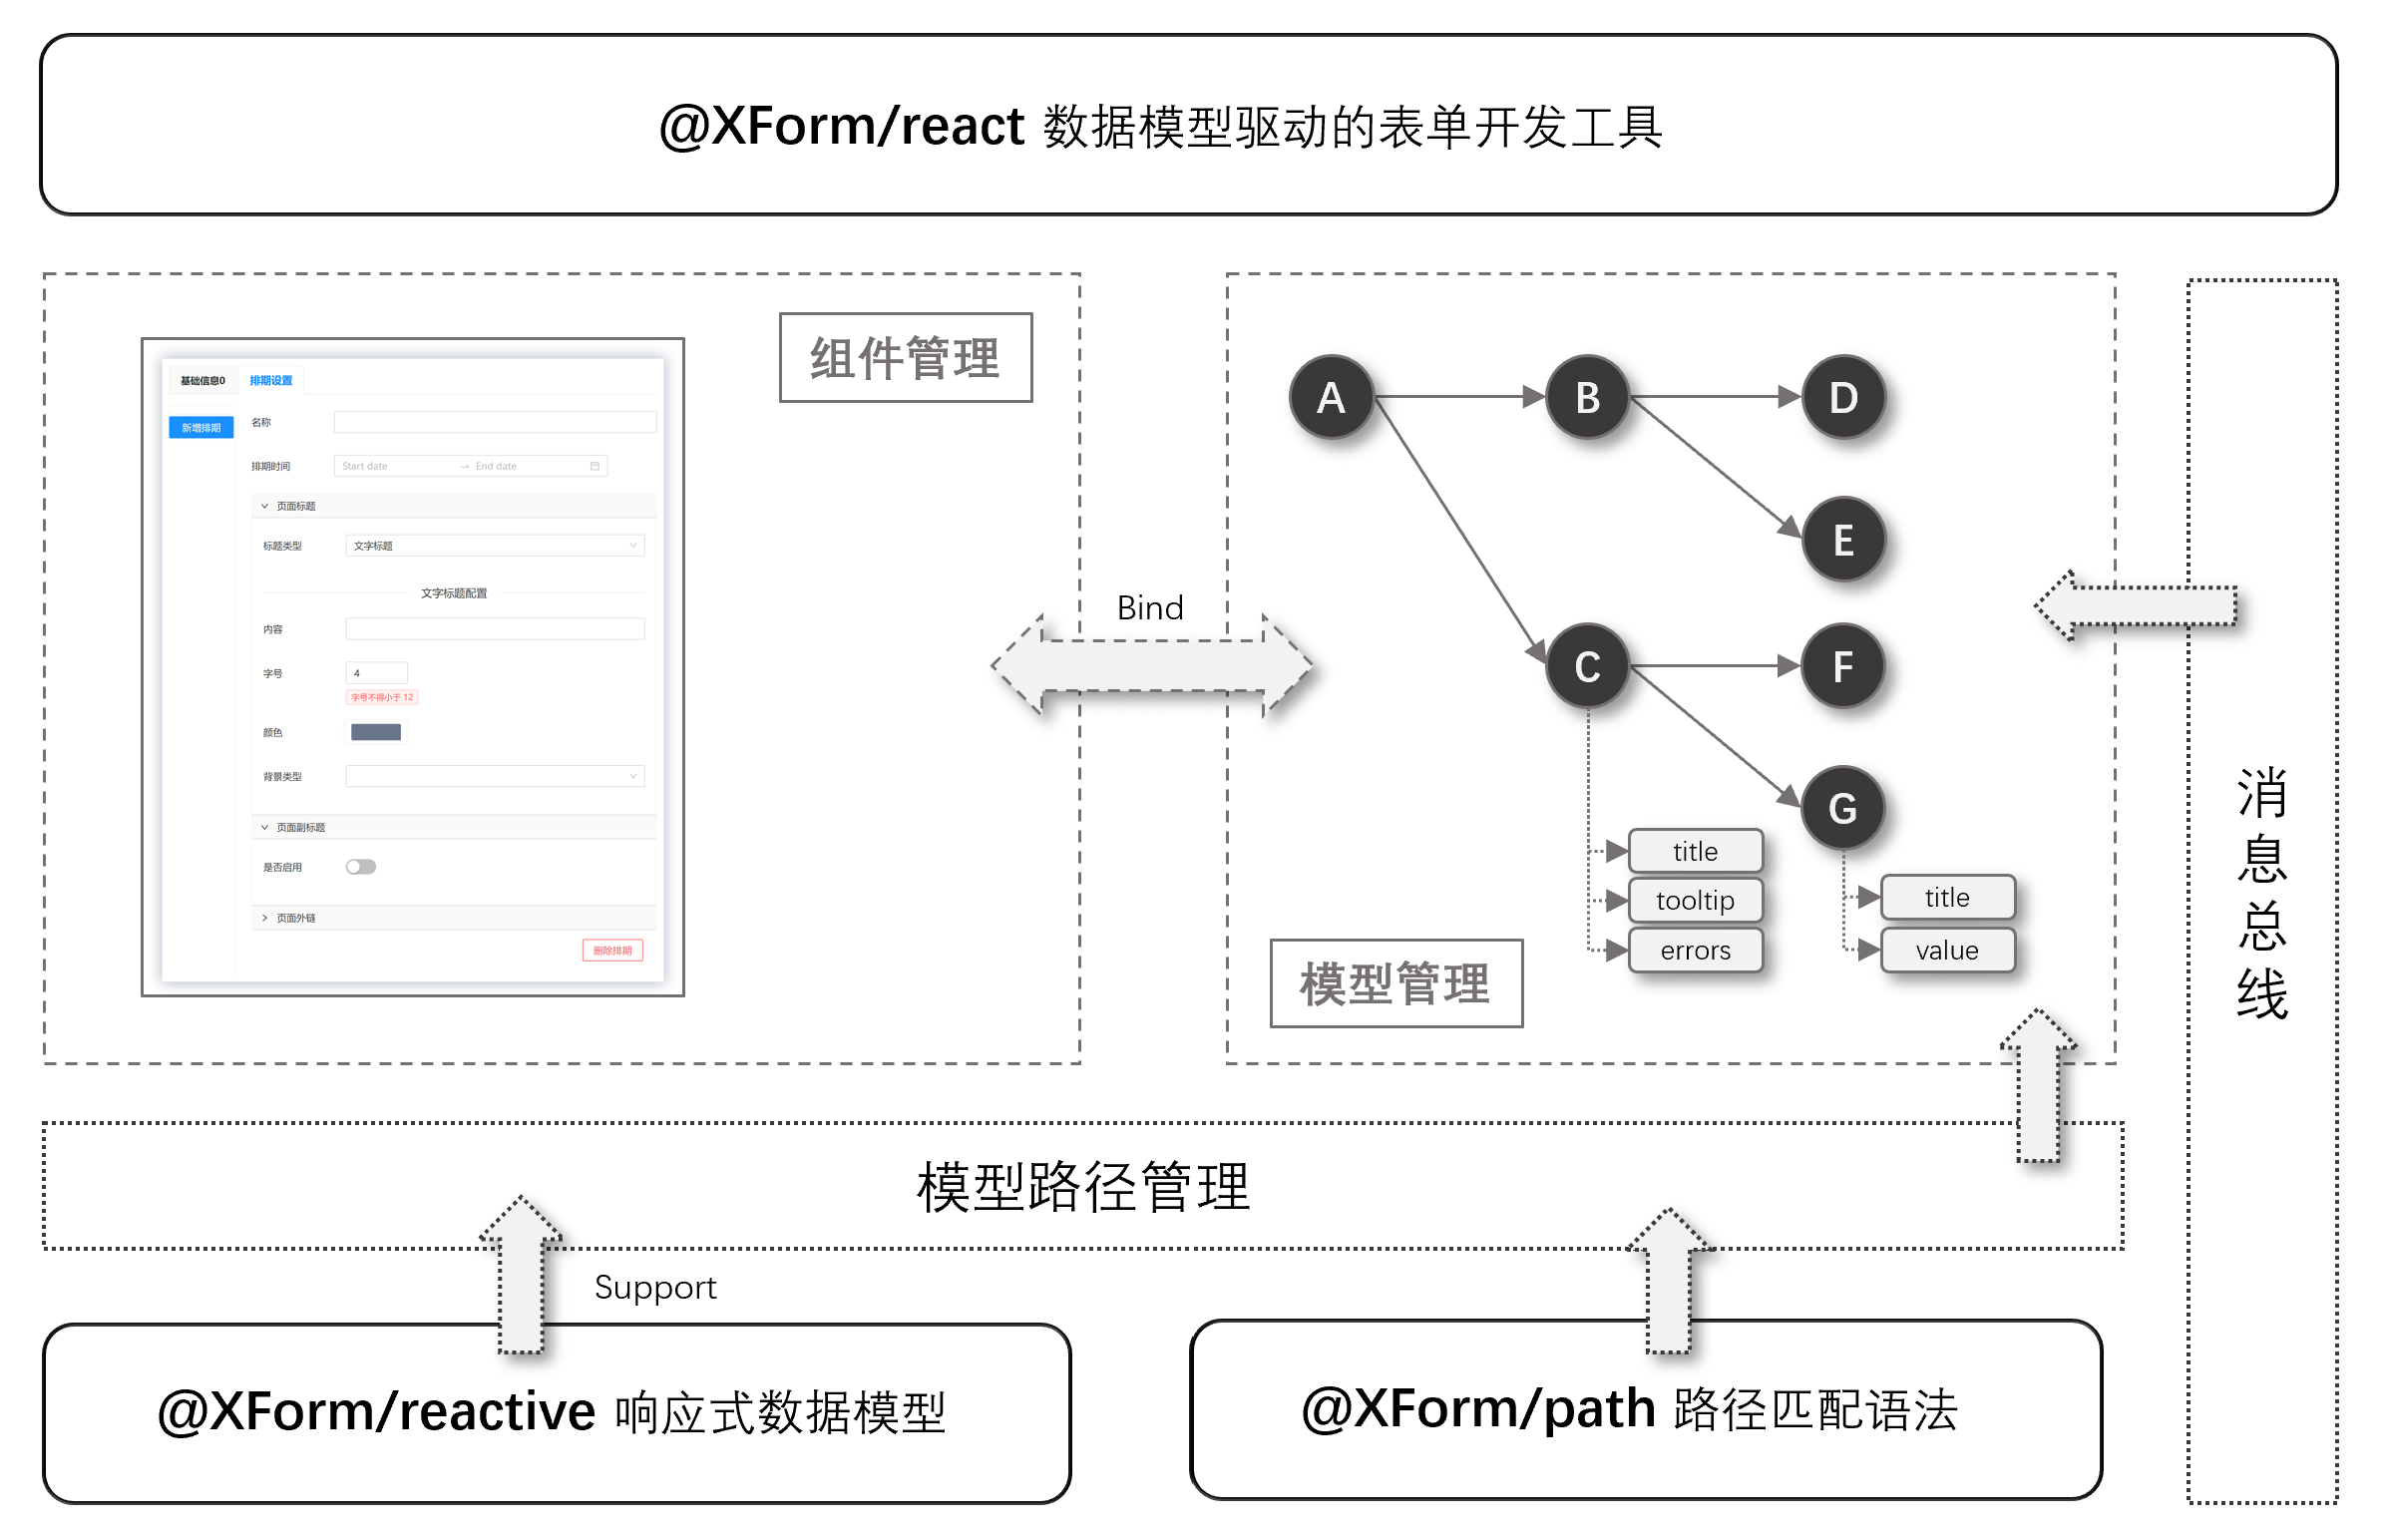
\includegraphics[width=\textwidth]{figure/chapter-4/overview-final-update.png}
    \caption{\xform{react} 完整架构图}
    \label{overview-final}
\end{figure}

如 \hyperref[final-solution]{3.3.2节}所述,组件渲染机制和数据模型管理一样,是表单开发的一个重要组成部分。因此为了实现完整表单开发的工具链,还需要结合\hyperref[reactive-datamodel-based-on-path-system]{第四章}所述的数据模型管理方案,针对前端框架进行相应的适配,完整的表单开发工具设计方案如\hyperref[overview-final]{图5-1} 所示。

具体来讲,适配工作要实现组件与数据模型的绑定,首先,按照 \hyperref[final-solution]{3.3.2节}给出的解决方案,这种绑定关系的粒度要细化到数据模型的字段变量和基础组件之间的一一对应,以实现组件的响应式更新\footnote{即变量变化时自动触发对应基础组件的重新渲染},这需要结合 React 框架的 API 进行针对性的优化;其次,为了提升开发效率,还需要简化字段对应复合组件的接口定义方式,以降低复合组件声明的代价。

% 具体来讲,适配工作首先需要实现组件的响应式更新\footnote{即变量变化时自动触发组件的重新渲染,也称作双向绑定},除此之外,为了提升开发效率,还需要尽可能地简化表单开发过程中定义字段、变量、依赖关系、组件绑定的接口。

\section{数据模型驱动的表单开发}

React 框架的适配工作有两个核心问题:

\begin{enumerate}
    \item 怎样结合响应式数据模型实现组件的响应式更新,实现对 React 渲染机制的适配
    \item 怎样将路径系统与基础组件高效地结合在一起,实现模型的分发
\end{enumerate}

\subsection{响应式组件}

如 \hyperref[react-framework]{2.1.2.2节}所述,React 最基本的 VDOM 重新渲染触发方法是更新 state,但是由于响应式数据模型是全局作用域,因此直接将模型赋值给 state 几乎等同于覆盖式更新的时间开销,所以需要规避 state 声明,采用其他方式来触发 VDOM 的重新渲染。React 框架针对这类需要精准控制 VDOM 渲染行为的需求提供了 React.memo API,简单来讲,经过 React.memo 封装的组件,其重绘行为完全由开发人员控制,利用这一机制,再结合响应式数据模型的依赖函数注册,就可以完成变量和组件的自动绑定,从而实现\textbf{任一变量更新时,仅与之绑定的组件会对应地更新,而其他组件不会受到任何影响}的效果。

封装响应式组件的思路大致如下:

\begin{itemize}
    \item 调用 \textit{React.memo} 方法封装目标组件 \textit{render},在目标组件上绑定 \textit{forceUpdate} 方法,以实现主动触发重绘,并使用 \textit{element} 字段管理当前的 VDOM 计算结果。
    \item 当封装组件首次被调用时\footnote{如前文所述,React 组件的本质是一个函数,因此是可被调用的},其执行过程中就会触发 \textit{element} 属性被重写的 \textit{get} 方法,并将 \textit{forceUpdate} 方法作为依赖函数注册,然后执行原始的目标组件函数 \textit{render},获取 VDOM ,并作为 \textit{element} 的结果返回,最终完成封装组件的首次渲染。
    \item 当封装组件依赖的变量变更时,\textit{forceUpdate} 方法就会被相应地调用,并再次触发 \textit{element} 属性的 \textit{get} 方法,此时 \textit{forceUpdate} 方法已经完成了依赖函数注册,则直接执行 \textit{render} 返回新的 VDOM。
\end{itemize}

结合响应式数据模型,理论上任何 React 组件都可以通过上述方式封装为响应式组件。响应式组件要求原始组件内部的数据状态使用响应式数据模型进行管理,因此第三方组件库并不能直接进行封装。但与此同时,组件完全是通过其数据接口进行属性注入的,所以只需要对数据接口进行一层简单的代理就可以适配第三方组件库了,此处以分别以完全使用响应式封装的 Input 组件和复用已有的 Item 组件\footnote{通常用于作为输入组件的容器,展示标题、输入提示、校验反馈等信息}为例说明两类组件的适配方案:

\begin{center}
    \begin{minipage}{0.45\textwidth}
        \lstinputlisting[label={reactive-input-component},style=component-example-style,caption={响应式 Input 组件},captionpos=b]{code/chapter-4/common-component-to-reactive-component.tsx}
    \end{minipage}\quad
    \begin{minipage}{0.45\textwidth}
        \lstinputlisting[label={reactive-item-component},style=component-example-style,caption={响应式 Item 组件},captionpos=b]{code/chapter-4/item-reactive-component.tsx}
    \end{minipage}
\end{center}

通过上述方案,响应式数据模型中的变量与组件进行绑定的问题得到了妥善解决,但是所有字段对应的响应式组件都通过直接访问全局数据模型来获取目标数据会造成大量不必要的依赖关系挂载,实际上每个响应式组件只与其对应的字段中的变量存在依赖关系,因此需要适配路径系统完成字段对应的数据模型(以下简称字段模型)的分发。

\subsection{路径上下文与模型分发}

如前文所述,\xform{core} 实际上已经提供了通过路径关键字直接获取字段模型的 API 即 \textit{get} 方法,因此模型的分发可以直接借助 \textit{get} 方法完成,具体地讲,可以通过封装特殊的 ReactField 组件\footnote{对应响应式数据模型的 Field 类,ObjectField 以及 ArrayField 采用类似的解决方案即可}完成模型分发,进而自动完成组件绑定,开发人员只需要注入复合组件的声明就可以实现完整的表单定义:

\lstinputlisting[label={entire-path-model-distribute},style=component-example-style,caption={考拉海购案例表单部分模型定义},captionpos=b]{code/chapter-4/entire-path-model-distribute.tsx}

这种方式解决了模型分发的问题,但依然存在缺陷,参考 \hyperref[reactive-data-model-context-free-dependency]{4.1.4节}的讨论,严格依赖上下文的定义方式会增加代码复用的难度,这一点同样适用于模型分发的场景。为了解决这个问题,就需要提供一种机制在运行时维护路径的上下文,自动地完成路径拼接,从而提高代码的可复用性。

React 框架为此类需要自动维护上下文的场景也提供了相应的 \textit{Context} API,\textit{Context} 是 React 框架中独立于 state 和 props 进行数据状态管理的 API,开发者可以全局创建多个 \textit{Context} 实例,然后在组件开发的任一层级声明一个 \textit{Context.Provider} 并注入数据后,其子组件树上的所有节点就能通过特定的 \textit{useContext} API 获取该数据\footnote{等价的 API 还有 \textit{Context.Consumer} ,本文为便于展示样例,使用 \textit{useContext} },需要注意的是,如果某个组件树上的同类 \textit{Context} 进行了多次声明,节点只能获取到最近的 \textit{Context} 中的数据。

由于表单模型本身是一个树型存储结构,因此路径上下文的维护可以从根节点开始自上而下地逐层完成分发,这与 \textit{Context} 机制高度契合,因此本文选择引入 \textit{Context} 实现这一功能,具体的方案大致如下:

\begin{enumerate}
    \item 为模型树中的每个字段维护其路径、字段关键字、模型三类信息,其中:关键字在字段内部本地存储,路径和模型使用 \textit{Context} 向子字段进行分发。
    \item 任一字段都可以获取到其父字段的路径和模型信息,此时存在两种选择,如果没有指定的路径,则直接继承父字段的路径与关键字进行拼接,否则使用指定路径与关键字进行拼接,从而获取对应的子模型。
\end{enumerate}

通过实现上述方案,\hyperref[entire-path-model-distribute]{代码5.3} 就可以做出如下改进:

\lstinputlisting[style=component-example-style,caption={基于路径上下文实现模型分发},captionpos=b]{code/chapter-4/derived-path-model-distribute.tsx}

除了模型结构的声明之外,数据模型还需要定义变量和依赖关系,本文将这两点也一并集成到了路径分发机制中,具体地讲,它们分别使用两个接口进行定义:

\begin{itemize}
    \item \textbf{state}:变量的初始状态声明。
    \item \textbf{reactions}:当前字段需要注册的依赖函数。
\end{itemize}

变量初始状态和依赖函数将在对应的字段初始化时自动完成注册,并注入到其关联的 Field 中,样例代码如下:

\lstinputlisting[style=component-example-style,caption={React Context},captionpos=b]{code/chapter-4/complete-model-declaration.tsx}

到此为止,一个数据模型驱动的表单开发设计方案就基本完成了,基于该方案,一个完整的表单组件开发流程大致可以分为以下几个步骤:

\begin{itemize}
    \item 通过事先的业务需求沟通确定后端所需的 JSON 数据格式。
    \item 按照 JSON 数据格式对表单进行建模,并在代码中对应地初始化表单模型(包括各类依赖关系)。
    \item 按照设计稿调整每个字段对应的组件实现。
\end{itemize}

自此,在这套方案下,数据模型中的任意变量都可以实现\textbf{一次定义,任意位置访问}的效果,开发人员在发生业务需求变更时可以不再花费大量的额外代价修改 state 和 props 的声明,因此表单的开发效率可以大幅提升。

\section{简化的复合组件声明}

通过观察考拉海购的表单案例,本文总结出了表单开发时,其复合组件实现过程的两个重要特点:

\begin{enumerate}
    \item 组件访问的变量集合通常是相互独立的
    \item 复合组件通常是使用嵌套的手段实现的
\end{enumerate}

考虑到字段对应的基础组件集合普遍存在共性\footnote{例如:ID 字段和名称字段仅在校验上存在差异,输入组件、容器组件、布局组件都是相同的},字段与复合组件一一对应的实现方式实际上会产生大量的重复代码,除此之外,组件内部的大量数据接口绑定都需要由开发人员手动实现,代码的可复用性也随之降低,这与响应式组件的设计初衷相违背。为了进一步提升开发效率,提升代码的可复用性,本文针对嵌套型的复合组件给出了声明式定义\footnote{声明式编程是一种编程思想,旨在通过简单的语法组合已有的功能接口来实现功能复合。相较于直接使用编程语言定义复合功能的方式,声明式编程能够大幅降低开发成本\footnote{antoy2005declarative}}的接口,允许开发人员通过声明组件数组自动地完成嵌套式复合组件的生成并完成与模型的绑定,基于这一接口,开发人员就可以更灵活地拆分重组基础组件以完成表单字段的组件开发,其简化效果如\hyperref[basic-nested-component]{代码5.6}、\hyperref[declarative-nested-component]{代码5.7} 所示。

\begin{center}
    \begin{minipage}{0.45\textwidth}
        \lstinputlisting[label={basic-nested-component},style=component-example-style,caption={复合组件定义},captionpos=b]{code/chapter-4/basic-nested-component.tsx}
    \end{minipage}\quad
    \begin{minipage}{0.45\textwidth}
        \lstinputlisting[label={declarative-nested-component},style=component-example-style,caption={声明式复合组件定义},captionpos=b]{code/chapter-4/declarative-nested-component.tsx}
    \end{minipage}
\end{center}

通过灵活地使用嵌套组件声明式接口,表单组件的开发流程可以优化为如下形式:

\begin{itemize}
    \item 通过事先的业务需求沟通确定后端所需的 JSON 数据格式。
    \item 按照 JSON 数据格式对表单进行建模,并在代码中对应地初始化表单模型(包括各类依赖关系)。
    \item 使用声明式语法嵌套地组合基础组件
    \item 若无可用的基础组件,则根据设计稿进一步定制
\end{itemize}

\section{本章小结}\label{chapter-4-conclusion}

本章系统地介绍了一套数据模型驱动的表单开发方案,层层递进地解决了基础组件的响应式更新、字段模型分发、声明式复合组件定义等问题,最终基于这些策略实现了表单开发工具 \xform{react},同时实现了渲染性能和开发效率的提升。

\chapter{实验评估}\label{experiment-examine}

为了评估响应式数据模型方案的性能,本文以 React 原生开发和传统的全局数据模型管理方案为参照,分别就\hyperref[kaola-activity-configuration-form-model]{表2-1} 所示考拉海购的案例表单模型的不同维度进行了实验,并预计通过分析这些实验的结果回答以下问题:

\begin{itemize}
    \item XForm 是否正确地还原了依赖关系并完成了模型与组件的绑定?
    \item XForm 在实现大规模的表单时是否存在渲染性能优势?
    \item XForm 在实现大规模表单时是否提升了开发效率?
\end{itemize}

\section{实验配置}

实验的环境参数如下:

\begin{table}[h]
    \centering
    \begin{tabular}{|l|l|l|}
        \hline
        CPU 型号        & 操作系统             & 浏览器              \\ \hline
        Intel i7-10875H & Windows 11 22000.556 & Chrome 99.0.4844.82 \\ \hline
    \end{tabular}
\end{table}

\section{实验设计}

实验总体设计包含以下三个部分:

\subsection{\xform{react} 可用性测试}

\begin{figure}[h]
    \centering
    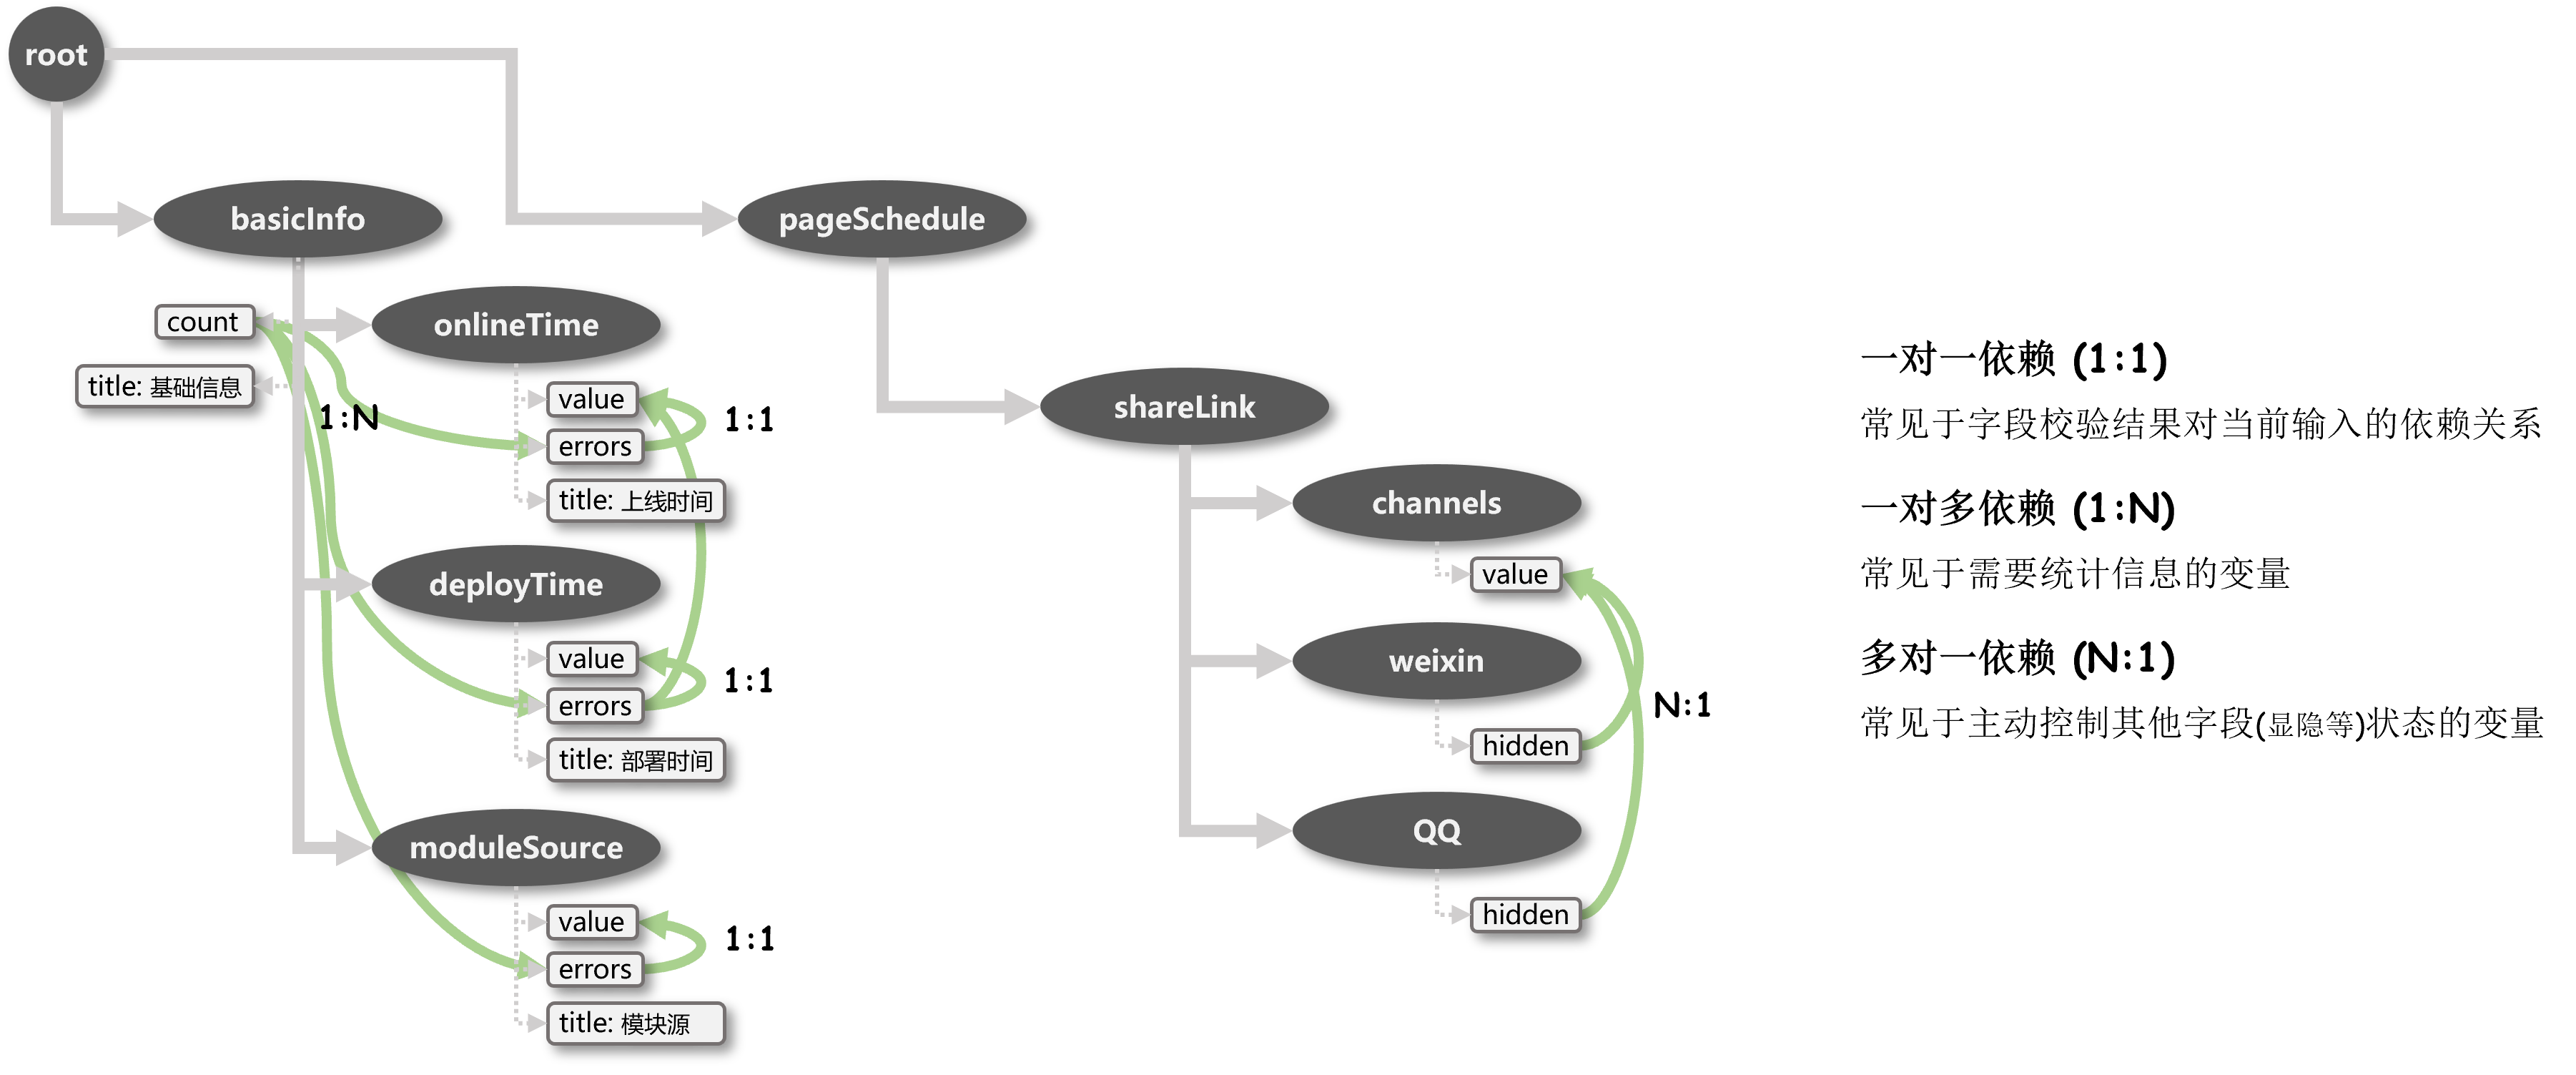
\includegraphics[width=\textwidth]{figure/chapter-5/usability-test-model.png}
    \caption{可用性测试模型概览及说明}
    \label{usability-test-model}
\end{figure}

结合\hyperref[problem-analysis]{第三章}的问题分析可知,表单开发的核心目标是实现组件和数据模型的统一,具体来讲,是实现数据模型内的字段变量和基础组件的绑定,在此基础上,其复杂性的根源来自变量间的依赖关系。

基于上述结论,本文为了验证 \xform{react} 的可用性,实现了完整的考拉海购案例表单,并重点对如\hyperref[usability-test-model]{图6-1} 所示模型内几个包含三种典型的依赖关系形式的字段进行了测试。图示模型对应的组件及渲染效果将在测试结果中详细展示。

考虑到三种基础依赖关系可以组合出任意的依赖关系形式,因此本文仅针对三类基础的依赖关系设计了对应的测试用例,以验证数据模型还原依赖关系的正确性,验证方式为:使用 \xform{react} 实现用例模型设计,模拟用户输入,查看依赖目标依赖关系是否得到了正确的计算和渲染反馈。

\subsection{\xform{react} 渲染性能测试}

根据 \hyperref[related-work-analysis]{3.2节}对相关工作的分析可知,尽管模型切分和模型一维化策略在渲染性能上存在一定优势,但是受限于设计缺陷,它们只能应对表单开发场景中的一部分数据模型管理需求,而不能应用于例如考拉海购的案例表单一类的复杂表单模型。因此本文主要使用以下三种方法完整地还原了考拉海购的表单案例以进行渲染性能测试\footnote{完整性的参考标准主要是依赖关系是否全部正确定义}:

\begin{itemize}
    \item \textbf{方法1 - XForm}:直接使用 \xform{react} 管理数据模型,完成组件绑定,应对各类复杂的表单场景。
    \item \textbf{方法2 - Vanilla}:使用原生的基于 state \& props 的方式进行表单开发,通过针对性地调整接口实现也能应对各种规模的表单模型。
    \item \textbf{方法3 - Global}:使用传统的全局模型结合覆盖式更新的策略来管理数据模型,至少保证功能的正确性。
\end{itemize}

此外,作为渲染性能的参考,本文使用基于模型切分策略实现的 react-final-form (记作\textbf{Final}) 完整地实现了考拉海购的案例表单\footnote{尽管 react-final-form 没有直接提供跨模型依赖关系定义,但本文为了参考渲染性能,额外封装了跨模型依赖关系定义的接口};使用基于模型一维化策略实现的 formily (记作\textbf{Formily}) 不完整地实现了考拉海购的案例表单\footnote{部分依赖关系无法定义}。

\subsection{\xform{react} 开发效率测试}

通过\hyperref[datamodel-driven-form-development-toolkit]{第五章}的描述不难看出,XForm 并没有大幅改变 React 框架的开发逻辑,所以组件的开发成本没有提高,但是由于简化了数据模型的管理方案,数据声明的成本大幅降低,开发人员不再需要花费大量的时间来调整数据接口声明,为了验证其中的开发效率提升效果,本文引入了 LOC\footnote{line of code,软件规模度量中最早应用的方法,核心思路是统计代码行数来一定程度上获取软件的规模信息\cite{tran2002measuring},但是该数值在不同的计算方式下存在明显差异,因此只能用于大致估计规模\cite{jones1985programming}} 和功能点\footnote{function
 points,通过分析系统的功能需求,结合加权统计来估算软件的规模信息\cite{matson1994software},根据具体的开发场景,功能点统计有很多的衍生方法}两个统计量来定量地分析开发代价,具体方案如下:

\begin{enumerate}
    \item \textbf{LOC}:直接统计表单定义的代码行数,该数值可以一定程度上直观地体现开发成本,但是并不精确,因此仅作为参考。
    \item \textbf{功能点}:参考 \hyperref[form-development-scene]{2.2节}的描述,数据模型定义的变更\footnote{通过阅读源码定位需要变更的数据声明,选择合适的方案来最小化数据模型的调整}是表单开发阶段耗时最多的操作,因此本文按照实践经验分别定义了三种方法管理数据模型的关键操作,将这些关键操作作为功能点指标进行统计,具体如下(统一权重为 1):
          \begin{itemize}
              \item 方法1 - XForm:一个 reaction 声明 / 一个上下文无关依赖函数定义
              \item 方法2 - Vanilla:一个 state 声明 / 一个 props 接口注入 / 一个依赖关系定义
              \item 方法3 - Global:一个数据模型 API 的调用
          \end{itemize}
\end{enumerate}

本文分别使用三种方法实现了考拉海购的案例表单模型,并对 LOC 以及上述关键操作的执行次数进行了全面的统计,以验证 \xform{react} 是否存在明显的开发效率提升。

\section{\xform{react} 可用性测试}

为了更精准地描述考拉海购案例表单模型中的依赖关系,本文引入了 \hyperref[node-path-match]{4.3.1节}的路径匹配模式语法,具体如\hyperref[dependency-patterns]{表6-1} 所示。

\begin{table}[H]
    \centering
    \scriptsize
    \begin{tabular}{|c|p{4cm}<{\centering}|p{7cm}<{\centering}|}
        \hline
        模式       & 说明                                          & 样例                                                                                                                                                                                    \\ \hline
        一对一依赖 & $A.a\rightarrow B.b$                          & $\text{"基础信息.模块源"}.errors\rightarrow\text{"基础信息.模块源"}.value$,即 “模块源” 字段的校验信息依赖于其当前的输入值                                                              \\ \hline
        一对多依赖 & $A.a\rightarrow \text{Set}\langle Node.Attribute\rangle()$ & $\text{"基础信息"}.errorCount\rightarrow\text{"基础信息.**"}.errors$,即 “基础信息” 字段的 errorCount 变量依赖于其所有孩子节点的校验信息                                                \\ \hline
        多对一依赖 & $\text{Set}\langle Node.Attribute\rangle()\rightarrow A.a$ & $\text{"页面排期[index].页面外链.*(!外链渠道)"}.visible\rightarrow\text{"页面排期[index].页面外链.外链渠道"}.value$,即所有 “XX分享样式” 字段的显隐状态都依赖于 “外链渠道” 字段的输入值 \\ \hline
    \end{tabular}
    \normalsize
    \caption{模型基础依赖模式测试用例}
    \label{dependency-patterns}
\end{table}

以下分别为三种依赖模式最终的渲染效果:

一对一依赖模式样例渲染效果如\hyperref[one-to-one-dependency-figure]{图6-2} 所示\footnote{输入值如果不通过校验则会出现错误信息提示}。

% \begin{figure}[h]
%     \centering
%     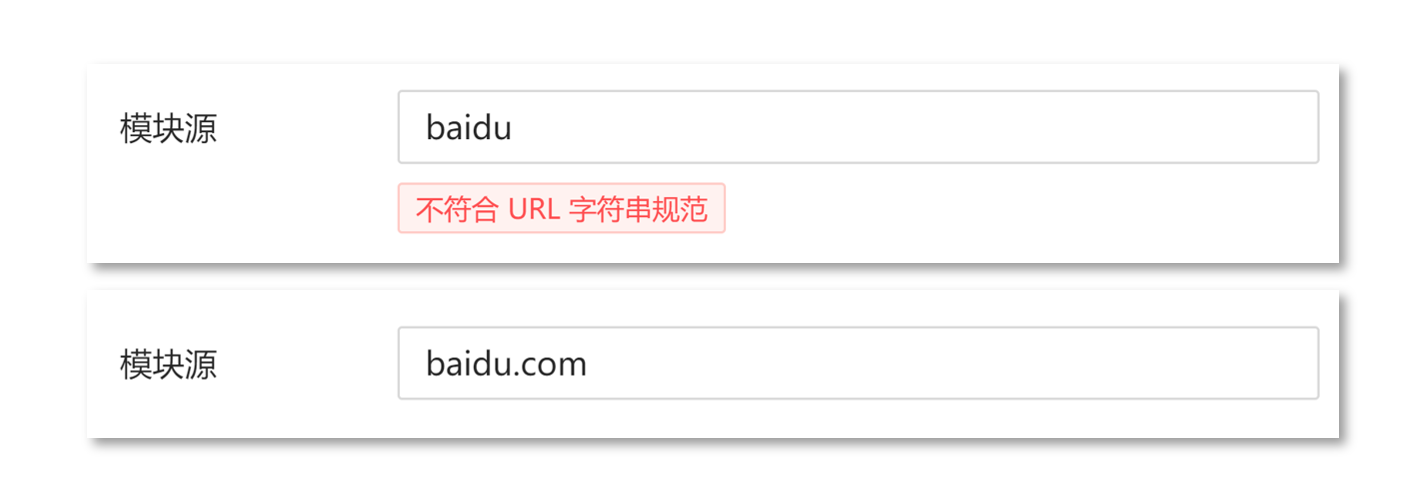
\includegraphics[width=\textwidth]{figure/chapter-5/one-to-one-dependency.png}
%     \caption{一对一依赖模式样例}
%     \label{one-to-one-dependency-figure}
% \end{figure}

一对多依赖模式样例渲染效果如\hyperref[one-to-many-dependency-figure]{图6-3} 所示\footnote{错误总数在样例图片的左上角使用红色圆形角标展示}。

% \begin{figure}[h]
%     \centering
%     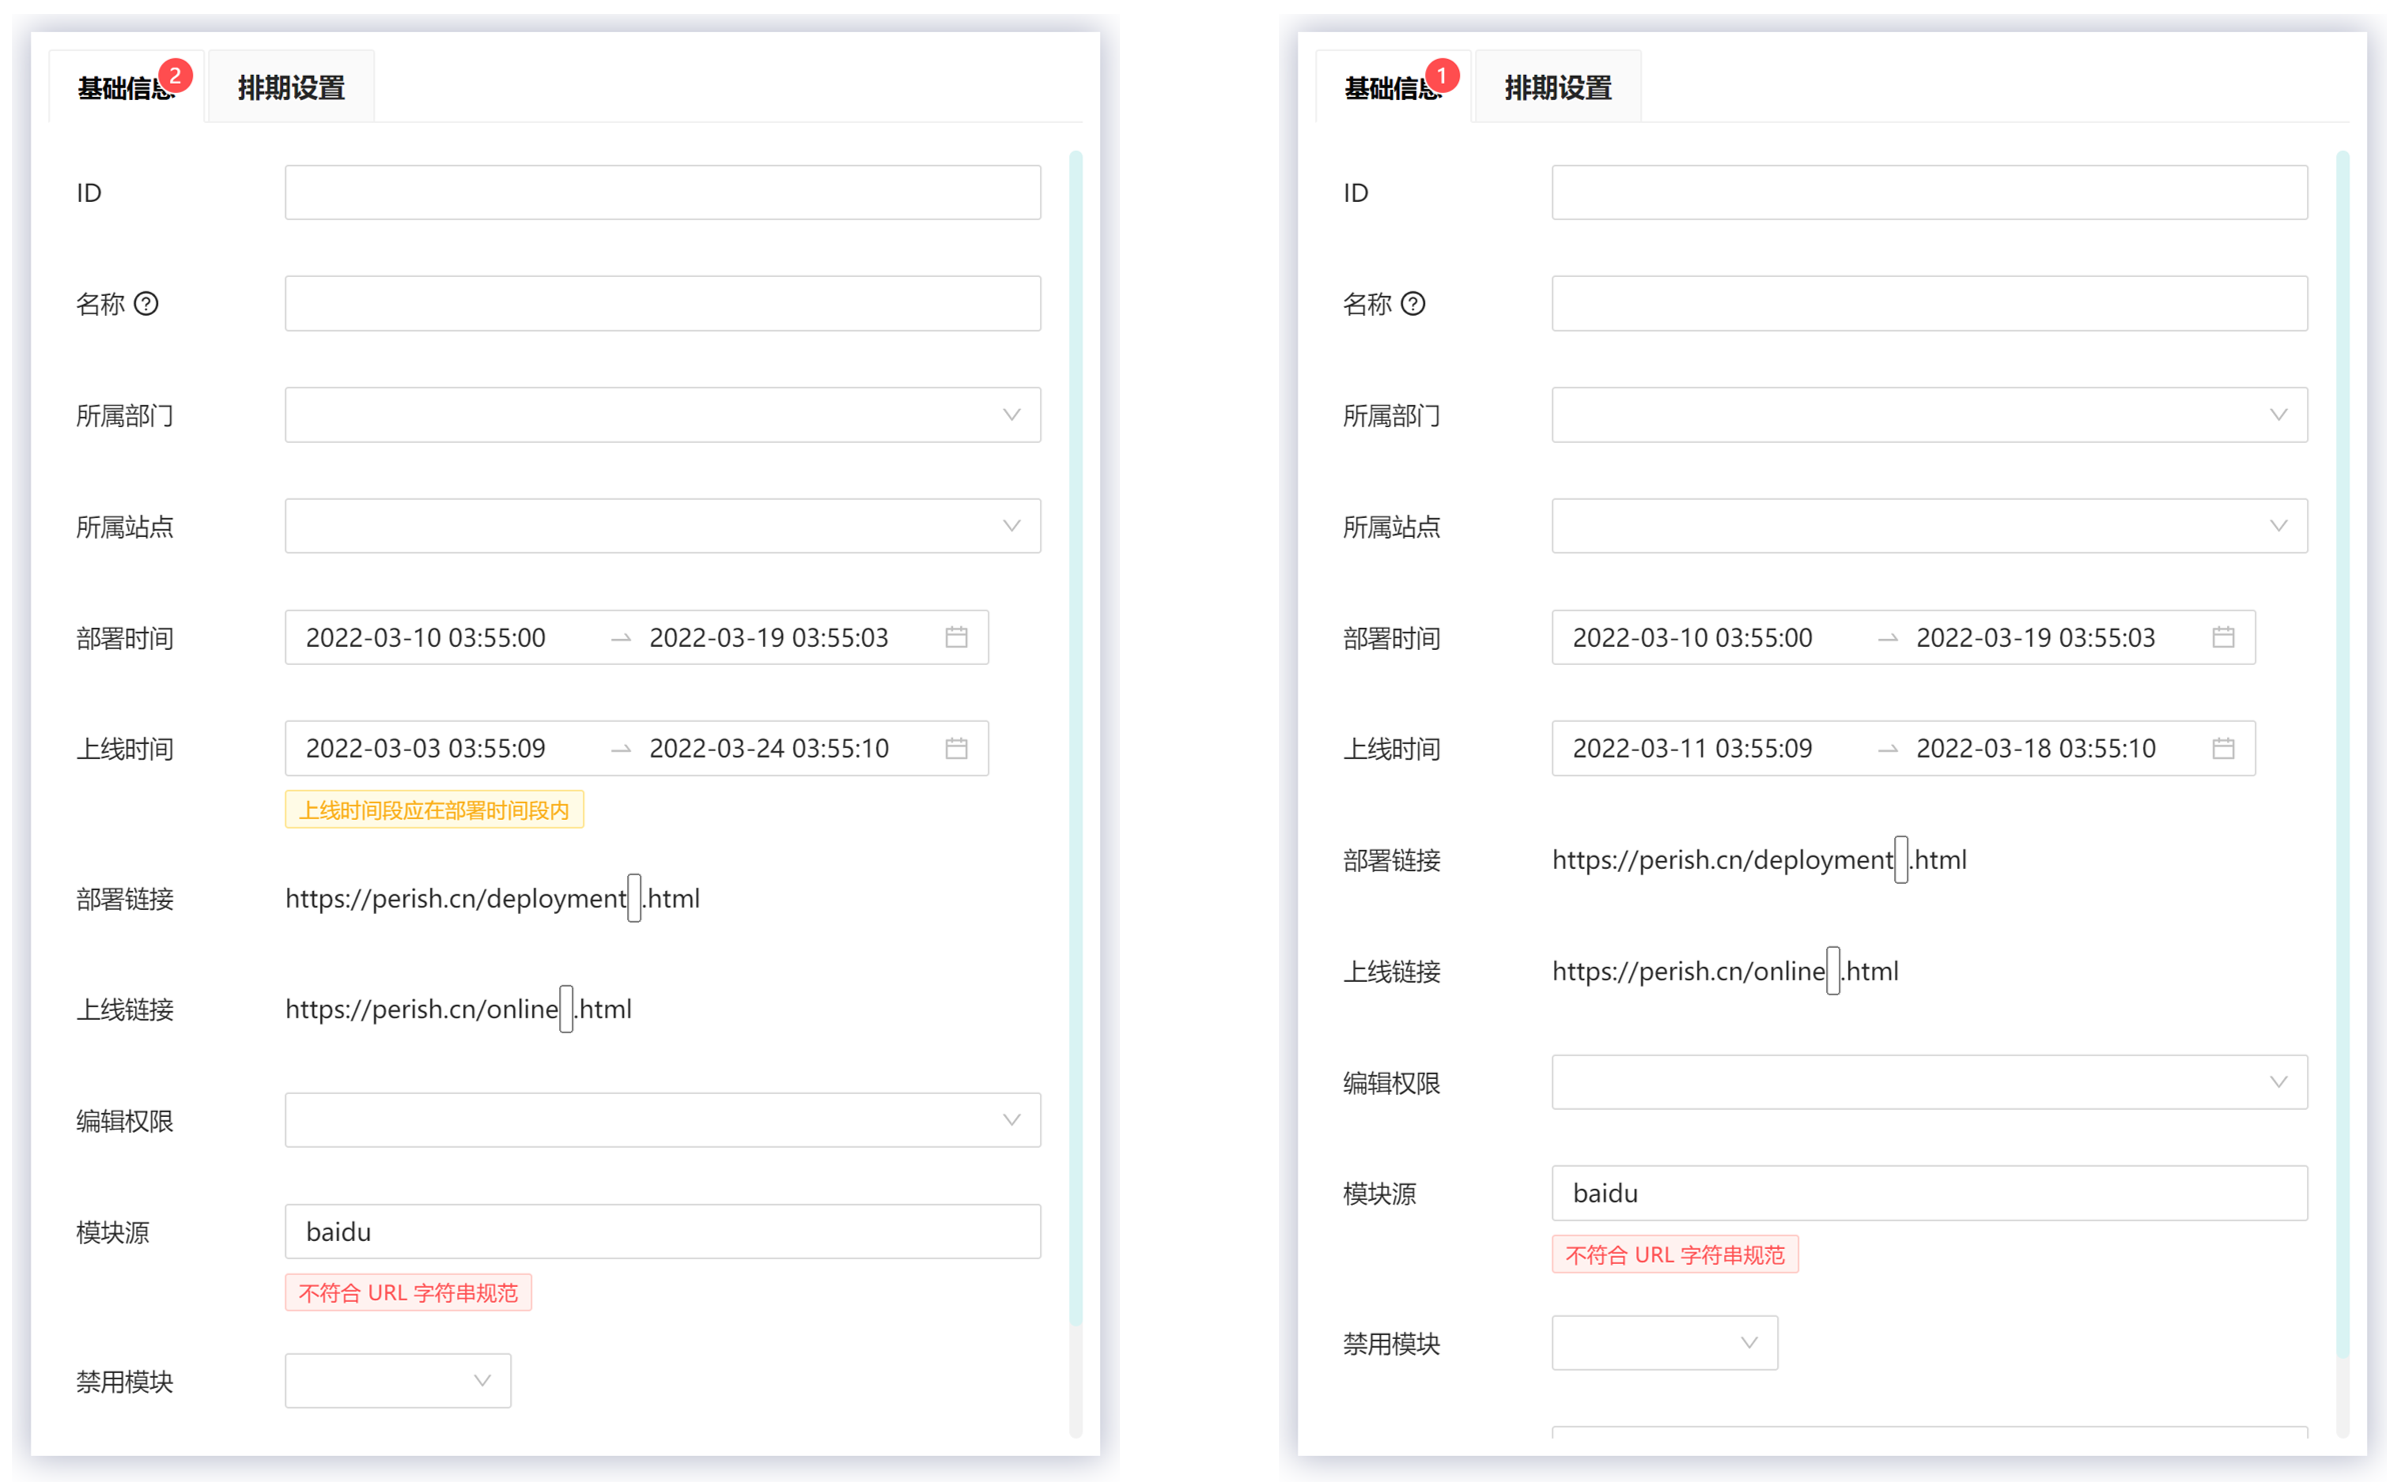
\includegraphics[width=\textwidth]{figure/chapter-5/one-to-many-dependency-update.png}
%     \caption{一对多依赖模式样例}
%     \label{one-to-many-dependency-figure}
% \end{figure}

多对一依赖模式渲染效果如\hyperref[many-to-one-dependency-figure]{图6-4} 所示\footnote{在多选框中的任意选项若被选中,则对应的分享样式填写内容就会变为显示状态,反之隐藏}:

\begin{figure}[h]
    \centering
    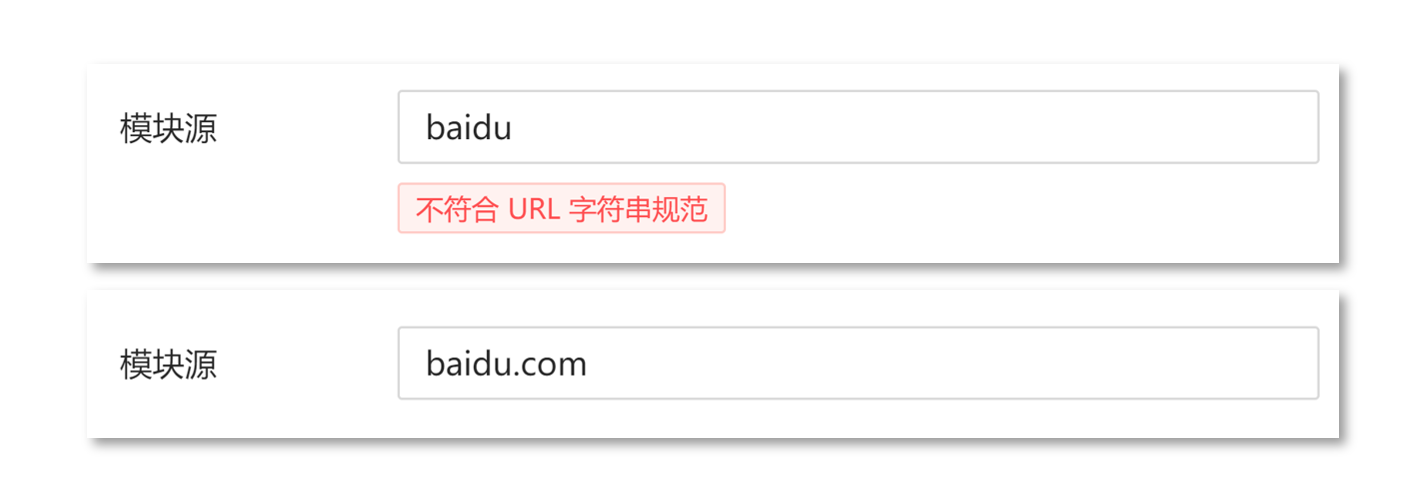
\includegraphics[width=\textwidth]{figure/chapter-5/one-to-one-dependency.png}
    \caption{一对一依赖模式样例}
    \label{one-to-one-dependency-figure}
\end{figure}

\begin{figure}[h]
    \centering
    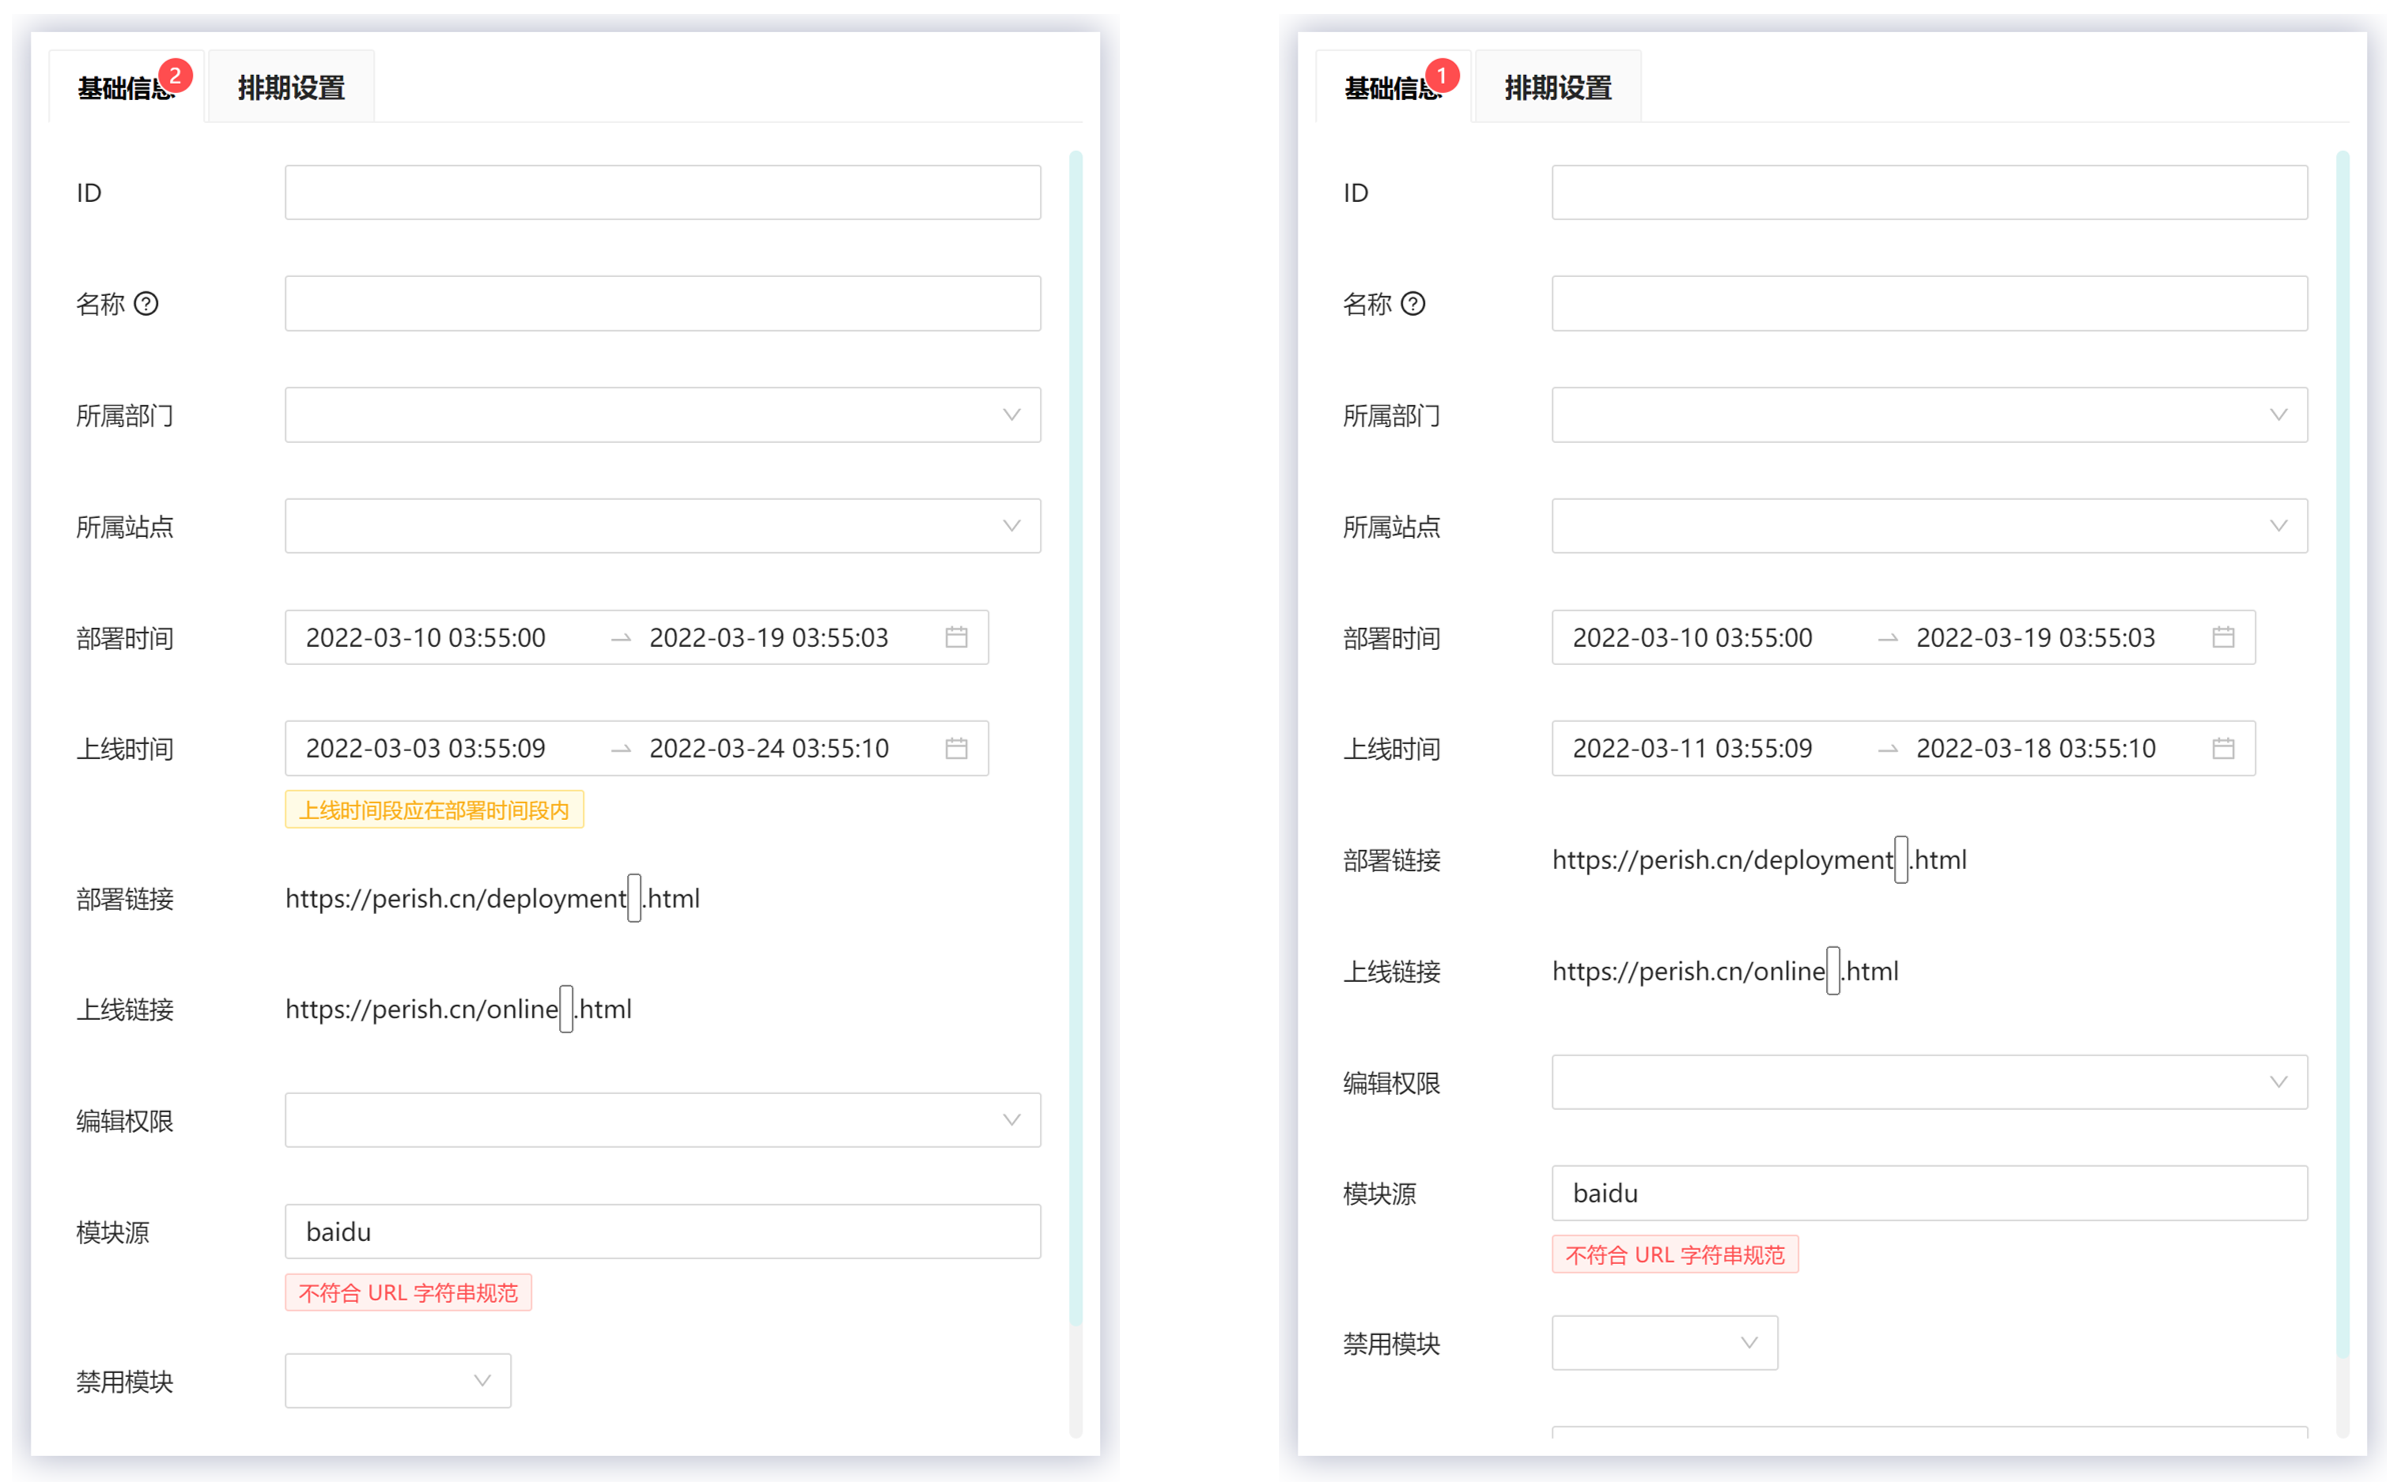
\includegraphics[width=\textwidth]{figure/chapter-5/one-to-many-dependency-update.png}
    \caption{一对多依赖模式样例}
    \label{one-to-many-dependency-figure}
\end{figure}

\begin{figure}[h]
    \centering
    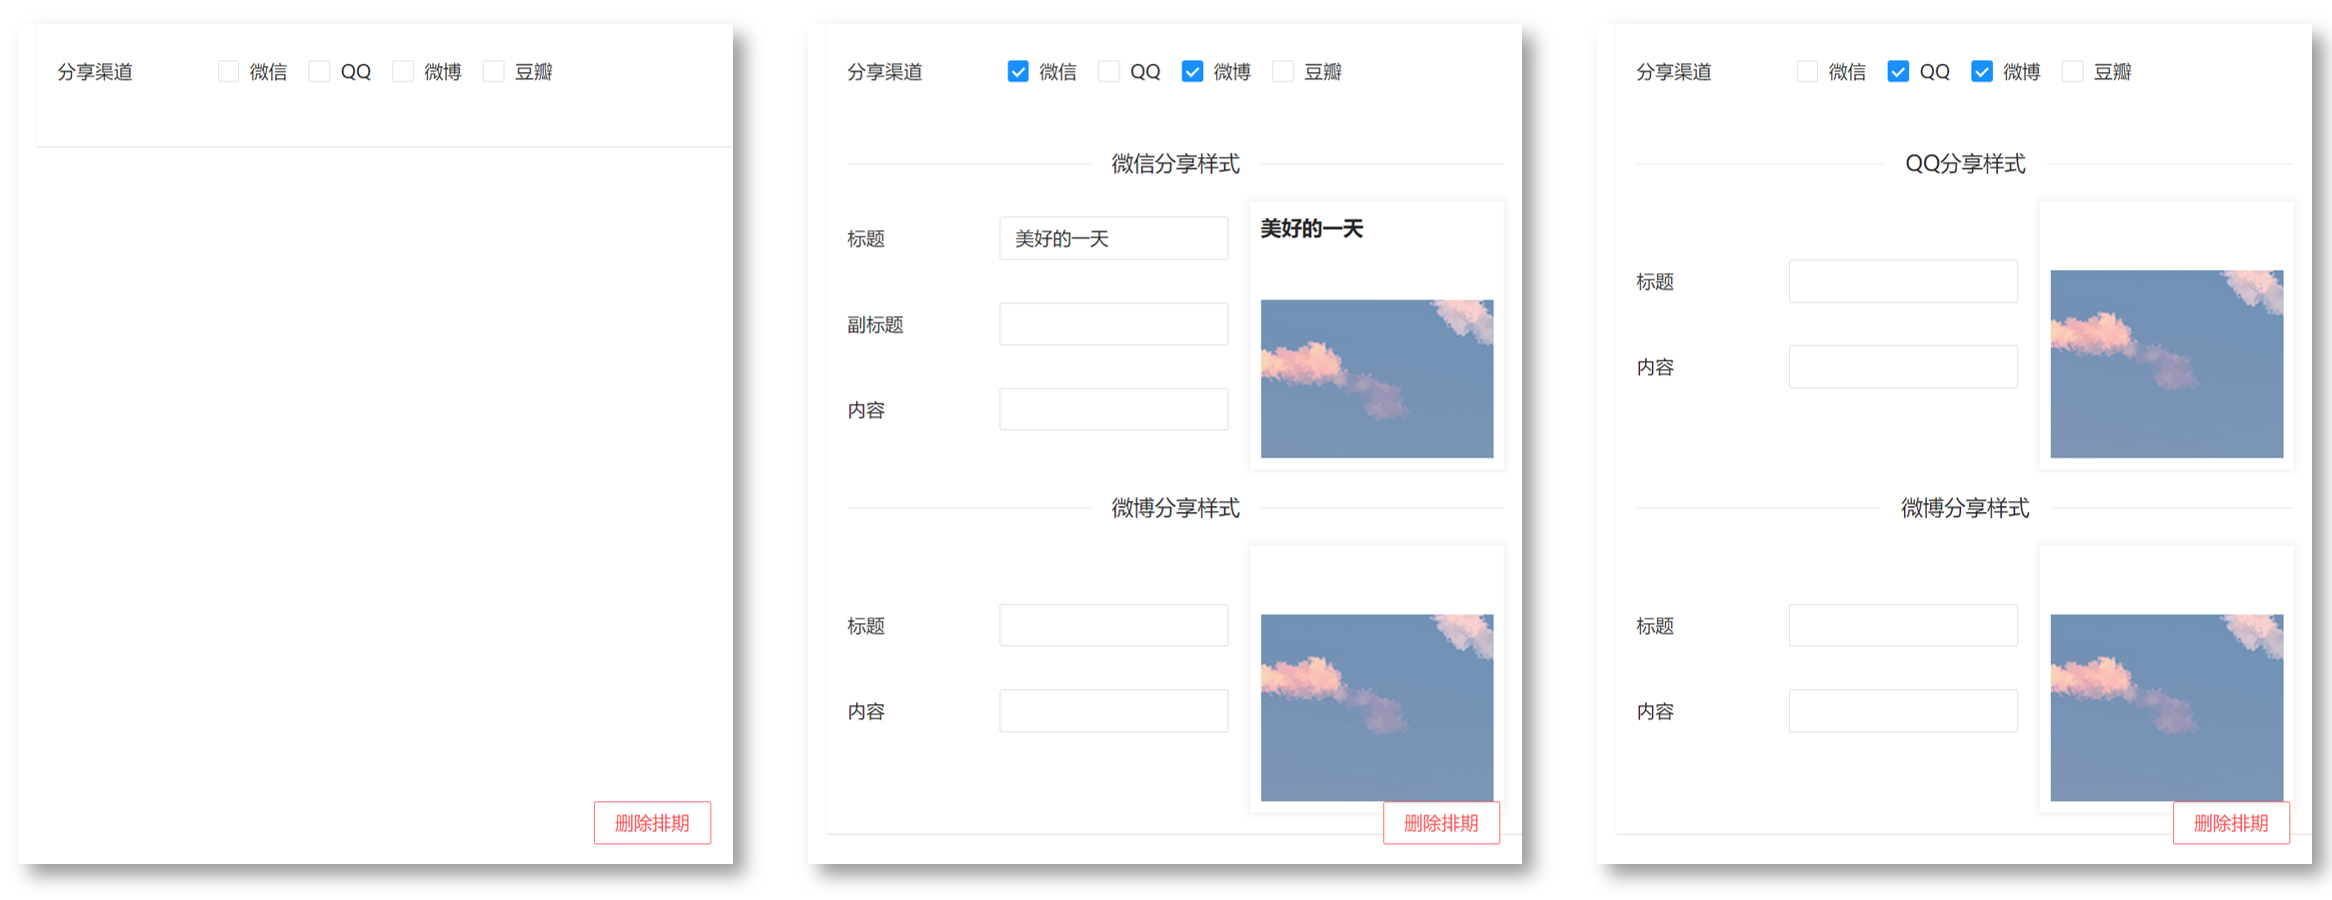
\includegraphics[width=\textwidth]{figure/chapter-5/many-to-one-dependency-update.png}
    \caption{多对一依赖模式样例}
    \label{many-to-one-dependency-figure}
\end{figure}

上述实验证明了 \xform{react} 能够正确地表达三类基本的依赖关系模式,它们可以通过进一步结合,衍生出链式依赖关系($A.a \rightarrow B.b\ \text{and}\ B.b \rightarrow C.c$)、多对多关系(many-to-one $\times$ one-to-many)等更复杂的依赖关系模式;同时,实验结果证明响应式组件正确地还原了数据模型和组件之间绑定关系,即变量的更改只影响其对应组件的渲染结果。因此,\xform{react} 保证了数据模型依赖管理以及组件渲染两方面的基础功能,其可用性得到了验证。

\section{\xform{react} 渲染性能测试}

渲染性能测试的基本流程是在 Chrome 浏览器中访问目标表单页面,使用 React 官方提供的 Profiling 工具进行录制,每一个输入操作模拟 20 次,取渲染时间的均值。Profiling 工具会自动记录用户输入触发渲染到渲染结束的各阶段信息,本文所用的信息 duration 是由 Profiling 工具自动计算的单次用户输入到渲染结束的时间间隔(不受两次用户输入时间间隔的影响),可以比较精准地反应真实渲染时间。

\begin{figure}[h]
    \centering
    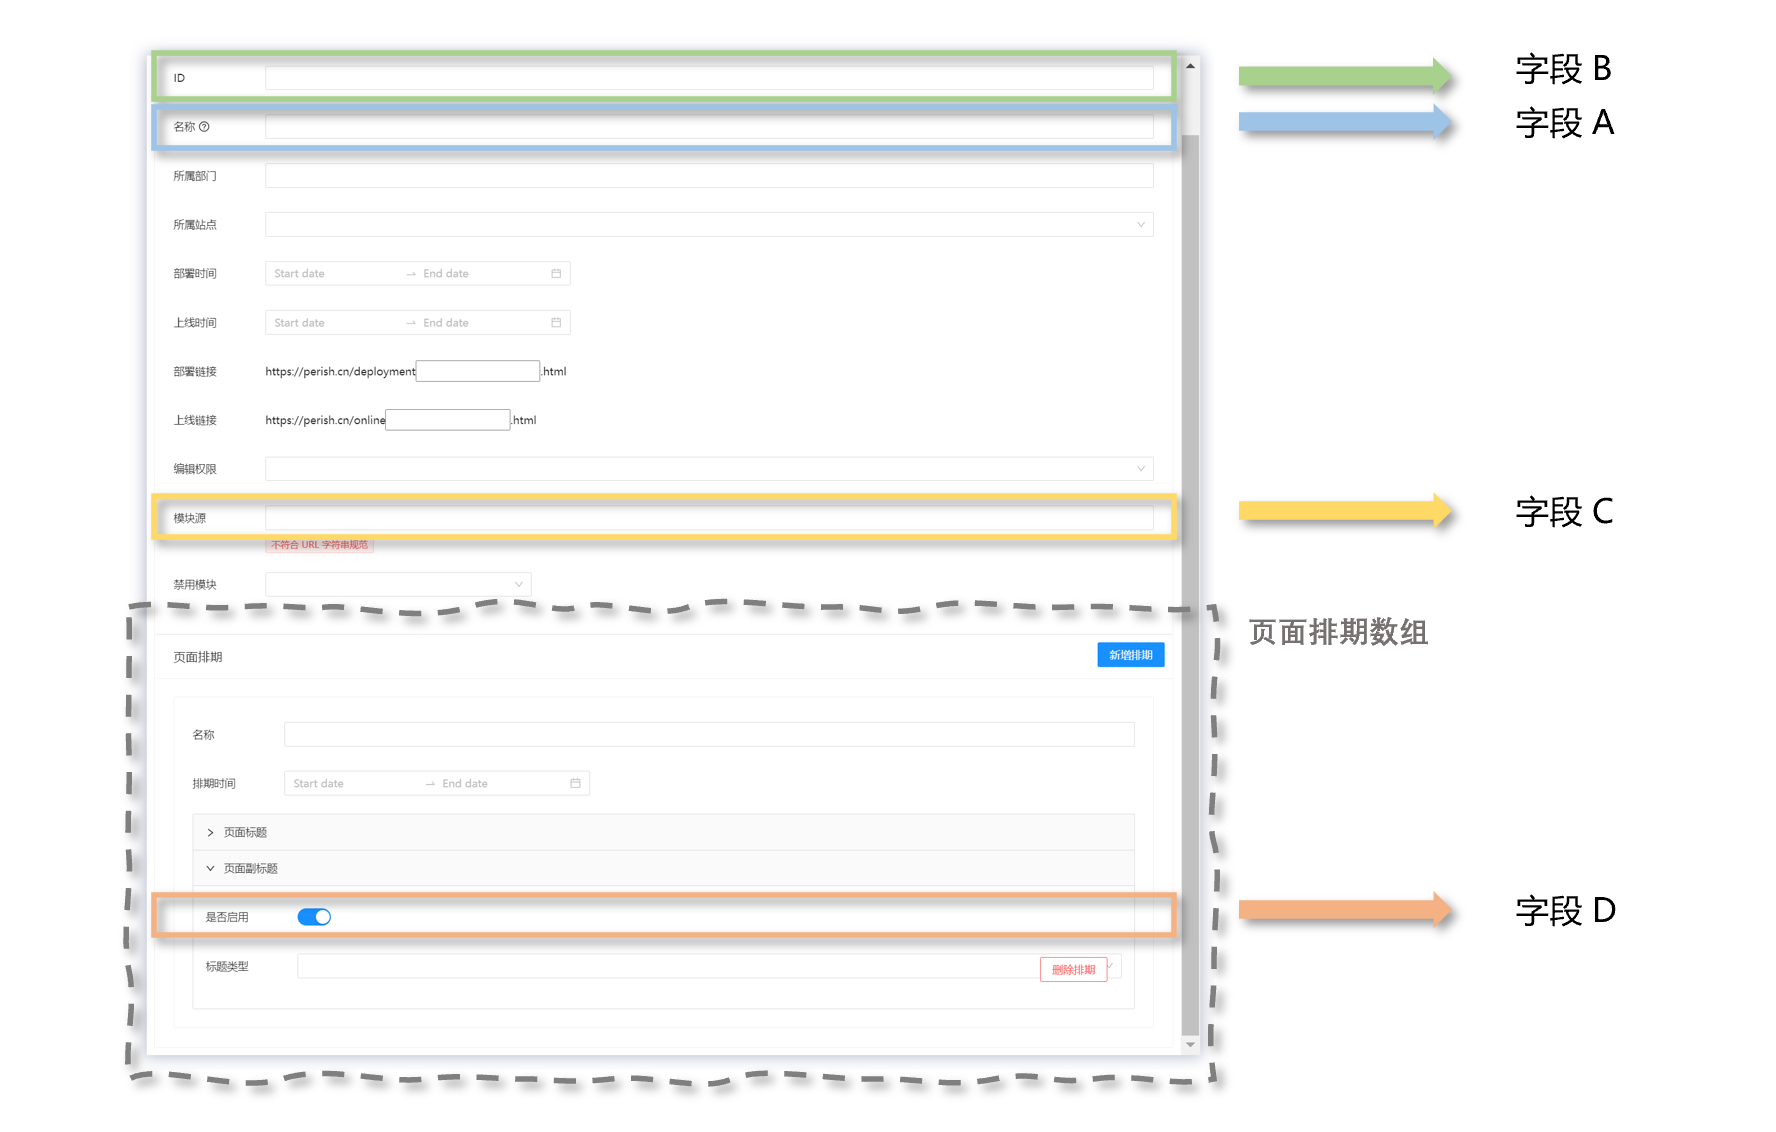
\includegraphics[width=0.9\textwidth]{figure/chapter-5/kaola-form-testcase-area-preview.png}
    \caption{渲染性能测试字段对应组件示意图}
    \label{kaola-form-testcase-area-preview}
\end{figure}

本文从考拉海购案例表单中选取了几个具有代表性的字段来模拟交互(参考\hyperref[kaola-form-testcase-area-preview]{图6-5}):

\begin{table}[h]
    \centering
    \scriptsize
    \begin{tabular}{|l|l|l|l|}
        \hline
        \multicolumn{1}{|c|}{编号} & \multicolumn{1}{c|}{目标字段}       & \multicolumn{1}{c|}{说明}              & \multicolumn{1}{c|}{操作方式} \\ \hline
        A                          & 基础信息.名称                       & 存在跨字段的一个依赖                             & 模拟用户输入                  \\ \hline
        B                          & 基础信息.ID                         & 存在跨字段的两个依赖                   & 模拟用户输入                  \\ \hline
        C                          & 基础信息.模块源                     & 存在同字段的一个依赖和跨字段的一个依赖 & 模拟用户输入                  \\ \hline
        D                          & 页面排期[index].页面副标题.是否启用 & 深度为 4 但为内部状态        & 模拟用户点击                  \\ \hline
    \end{tabular}
    \normalsize
    \caption{表单渲染性能测试样例设计}
    \label{kaola-render-performence-testcases}
\end{table}

为了证明表单内的变量个数对渲染性能的影响,测试过程还会将\textbf{页面排期}字段的数据项个数作为变量,分别在数组长度为 1,10,20,30,40,50 的情况下\footnote{单个\textbf{页面排期}字段的数组项包含约 24 个变量}进行上述字段的渲染性能测试,实验结果如下:

\subsection{字段A测试结果}

\begin{figure}[h]
    \centering
    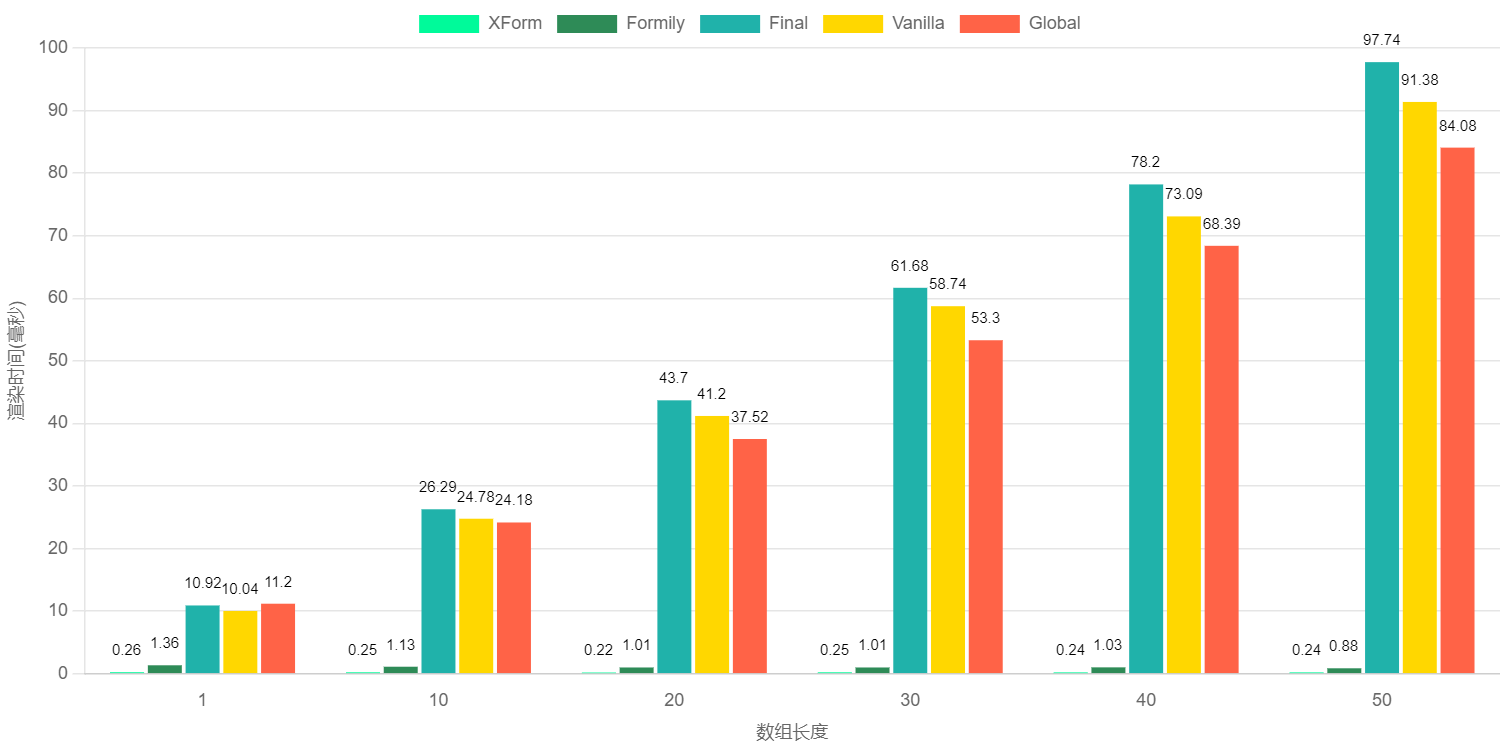
\includegraphics[width=\textwidth]{figure/chapter-5/A-update.png}
    \caption{字段A的渲染性能测试}
    \label{render-performence-testcase-A}
\end{figure}

从对字段A的测试结果可以看出,对于无依赖关系的字段,Vanilla 和 Global 方法的渲染时间整体随变量数增加呈线性增长,且数值差异很小;而不考虑测量误差, XForm 方法的渲染时间几乎是相同的,其渲染性能较另外两种方法存在几个数量级的提升,并且与 Formily 方法保持相近的渲染性能,这与 \hyperref[final-solution]{3.3.2节}的建模结论一致。而对于 Final 方法,可以看出在实现含跨模型依赖关系的表单模型时,由于模型切分策略在管理数据模型时引入了额外的数据操作,其渲染时间略长于 Global 方法。

\subsection{字段B测试结果}

\begin{figure}[h]
    \centering
    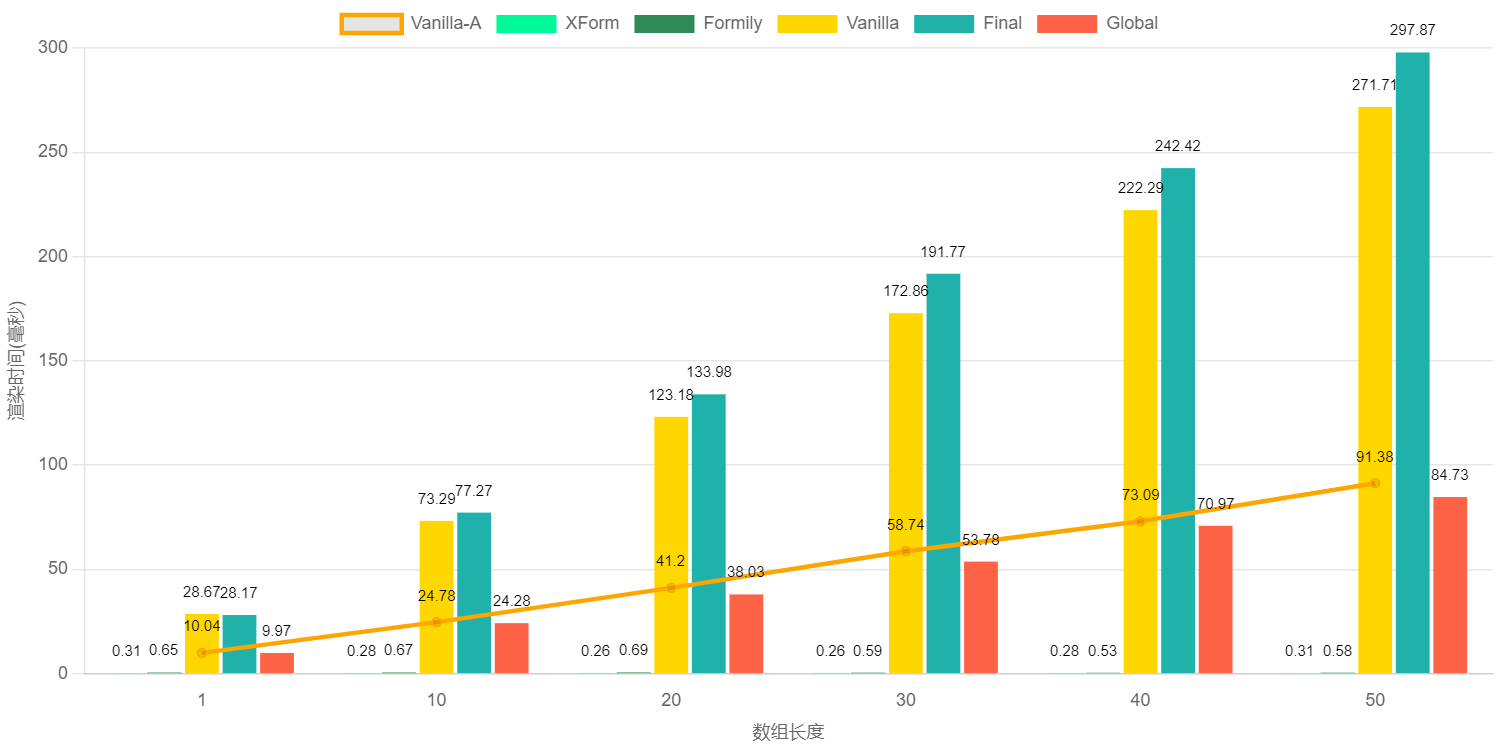
\includegraphics[width=\textwidth]{figure/chapter-5/B-update.png}
    \caption{字段B的渲染性能测试}
    \label{render-performence-testcase-B}
\end{figure}

从对字段B的测试结果可以看出,对于存在依赖关系的字段(样例中共有三个字段相互关联),Vanilla 方法和 Global 方法依然呈线性增长,进一步观察可以注意到,与字段A的测试结果相比较,Vanilla 方案由于需要分别进行三次 diff 操作,因此恰好存在约 3 倍的渲染开销,而 Formily 方法与 Final 方法的结论与字段A一致。

与字段A的测试结果相同的是,XForm 方法依然保持稳定的性能优势,这里需要说明的是,由于依赖关系涉及到的节点数太小,因此 XForm 方法的渲染时间已经接近了 Profiling 过程完成插桩和统计的时间,很难区分字段A与字段B的开销差异;而 Global 方法的全局更新策略使得其应对不同字段均保持了相近的渲染时间,这种方法在不考虑优化的情况下甚至优于 Vanilla 方法。

\subsection{字段C测试结果}

\begin{figure}[h]
    \centering
    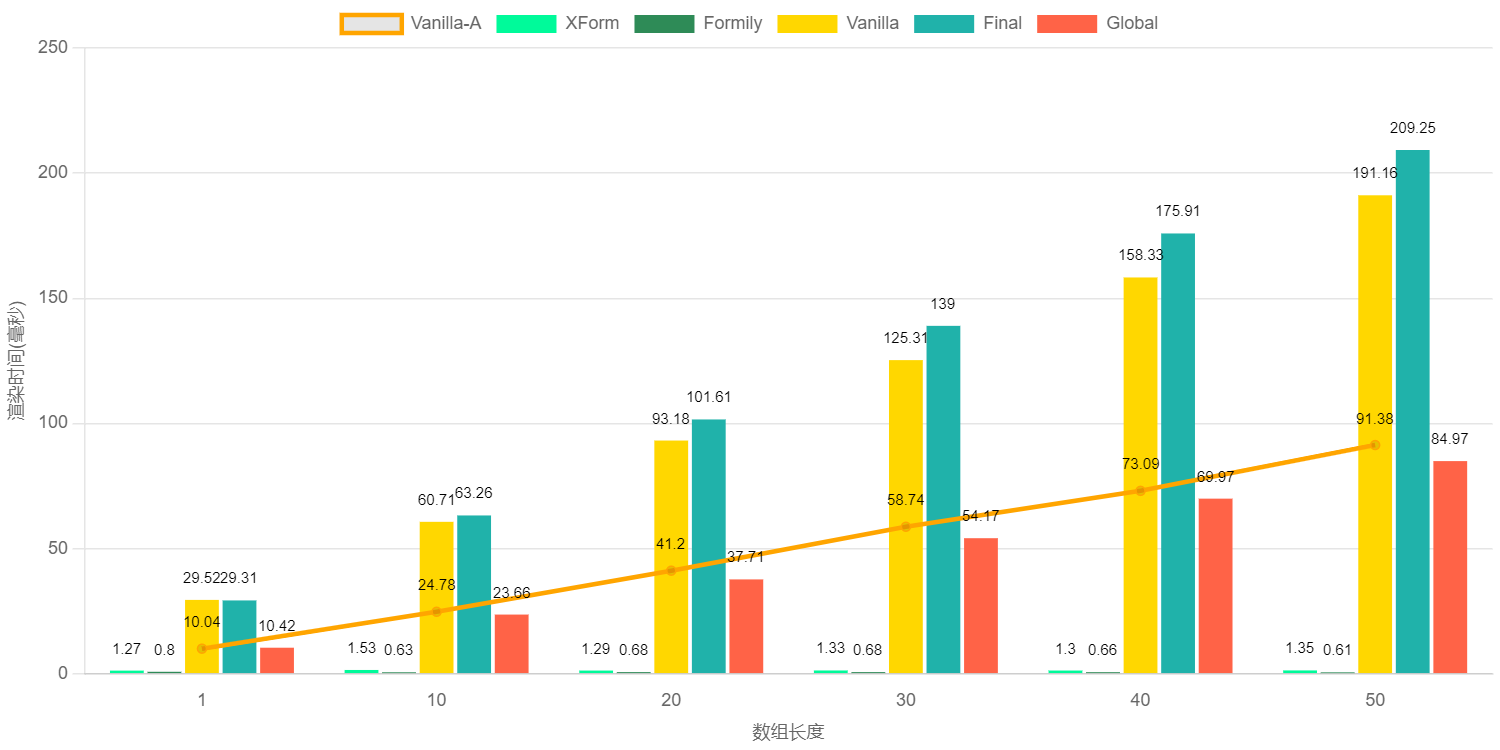
\includegraphics[width=\textwidth]{figure/chapter-5/C-update.png}
    \caption{字段C的渲染性能测试}
    \label{render-performence-testcase-C}
\end{figure}

与字段B相似,字段C的测试结果中,XForm 保持稳定性能优势;Vanilla 方法并没有受到依赖关系中节点层级的影响,恰好保持约 2 倍于字段 A 的渲染开销;Global 方法和 Final 方法保持稳定的开销变化;但是 Formily 方法无法表达此类依赖关系,因此只能展示不含依赖关系的情况下的渲染时间。

\subsection{字段D测试结果}

\begin{figure}[h]
    \centering
    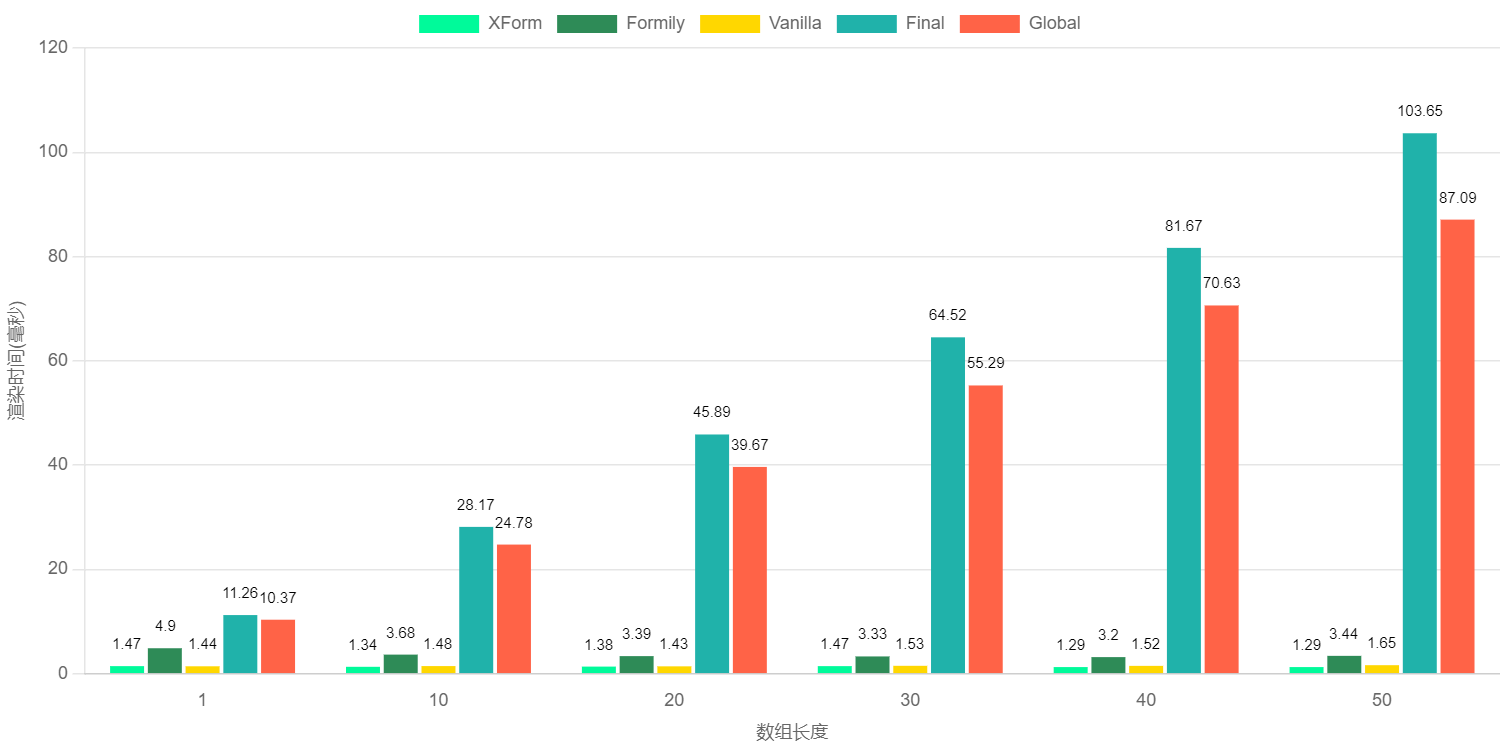
\includegraphics[width=\textwidth]{figure/chapter-5/D-update.png}
    \caption{字段D的渲染性能测试}
    \label{render-performence-testcase-D}
\end{figure}

在字段D的测试结果中,XForm 方法与 Vanilla 方法呈现了几乎一致的高渲染性能,而 Global 方法却维持与字段A相近的渲染开销。这是由于 Vanilla 方法使用 state (即内部状态) 对该字段的值进行管理,从而最小化了受影响的组件范围,当然代价也是有的,由于使用 state 进行封装,因此目标属性是外部不可访问的,未来发生可能的需求变更时,该属性还需要转换为 props 声明,从父组件注入,修改代码的同时还会增加渲染的时间开销。

\subsection{渲染性能测试总结}

从四类典型字段的测试结果可以看出,XForm 方法具备极佳的渲染性能,不仅在单变量的情况(字段D)下能够实现与 Vanilla 方法几乎一致的渲染性能,而且变量规模较大的特定场景下,甚至能达到超过 100 倍的性能提升。

根据 Card 等人的研究结论\cite{card1991information},100ms 可以认为是用户感知交互是否 “卡顿” 的一个临界点,从测试结果可以看出,Vanilla 方法的部分测试结果已经远远高于这一数值,Global 方法也达到了约 85ms 的渲染时间,可以预见随着变量数增加,模型规模扩大,两种方案都会出现渲染性能瓶颈,而 XForm 方法在四项测试中均稳定保持 1 毫秒级的渲染时间,因此能够广泛适用于各种规模的表单模型。

\section{开发效率测试}

三类方法的 LOC 和功能点数量通过人工统计的方式得出,其结果大致如下:

\begin{table}[h]
    \centering
    \begin{tabular}{|l|l|l|l|}
        \hline
                 & XForm & Vanilla & Global \\ \hline
        LOC      & 802   & 878     & 826    \\ \hline
        功能点 & 22    & 108     & 86     \\ \hline
    \end{tabular}
    \caption{表单开发效率统计}
\end{table}

首先需要强调的是,由于原始的考拉海购案例表单模型过于复杂,涉及到大量的基础组件定制,因此本文并未对其作 1:1 的还原,具体到代码实现上,每个字段对应的组件平均简化了两个层级,另外部分与内部系统强相关的涉密内容也作了剔除;其次,本文仅统计了表单定义部分的代码,而略去了基础组件开发、测试环境搭建以及整个开发过程中所有可复用 API 的代码。

最终从统计结果来看,XForm 方法在 LOC 指标上存在较小的优势,考虑到组件的嵌套层级较浅,因此嵌套组件的声明式接口没有体现明显的优化效果,该结果符合预期;与此同时,XForm 相较于另外两种方法极大地降低了关键操作的次数\footnote{Global 方法较 Vanilla 方法在功能点指标上也存在一定的优势,但是远低于 XForm 方法的提升},这意味着开发和修改的代价均得到了有效的控制,开发效率和代码可维护性大大提升。

\section{本章小结}

本章围绕考拉海购的表单案例设计了一系列实验用于验证 \xform{react} 是否可用,以及在渲染性能、开发效率上是否存在明显的提升效果。最终,实验结果证明 \xform{react} 能够正确地还原含有复杂依赖关系的表单模型,并且在渲染性能和开发效率上与相同功能集的另外两类表单开发方法有显著优势。

\chapter{总结与展望}

\section{工作总结}

首先,本文针对前端开发中的表单开发场景,介绍了前端框架开发的基础知识,并结合考拉海购的实际表单案例描述了表单开发复杂性的根源,随后以数据模型管理为切入点,给出了一套完整的表单开发建模方法并基于该方法介绍了相关工作的解决方案以及它们的优缺点,并进一步总结了表单数据模型管理应当解决的核心问题。

然后,本文自底向上地介绍了一整套数据模型管理方案,分别解决了三个核心问题:响应式更新、逻辑结构维护、多字段依赖定义,并最终基于该方案实现了数据模型管理工具\xform{core}。

接下来,本文基于\xform{core}针对 React 框架进行了全面适配,实现了数据模型驱动的表单开发工具\xform{react},并提供了响应式组件、模型分发、声明式复合组件三个核心功能,完善了表单开发的工具链。

最后,本文使用包括 XForm 在内的五类表单开发方法分别实现了考拉海购的案例表单,并从不同的维度设计了一系列实验,实验结果证明,XForm 方案可以用于管理存在复杂依赖关系的表单模型,并且在渲染性能和开发效率上,较相关工作有显著优势。

\section{研究展望}

以下是本文在研究过程中关于后续研究方向的一些思考:

\begin{itemize}
    \item \textbf{深入前端开发领域}:表单开发是前端开发的一个典型场景,几乎囊括了前端开发可能出现的所有需求\footnote{这里的前端开发是狭义的,仅指代基于 DOM API 进行的页面开发},因此表单开发的解决方案存在推广到整个前端开发领域的可能性,这可能成为后续研究的一个切入点。
    \item \textbf{HTML Table}:table 是 HTML 标准中用于描述二维表格的标签,在表单场景中也有非常广泛的应用,由于 table 标签抽象层次较低,因此往往需要使用第三方工具来简化 table 在布局(行、列、单元格合并、固定表头、...)上的声明,而这类工具底层采用的数据模型管理方案也普遍是全局覆盖的策略,从根本上限制了 table 的渲染性能,如果应用类似 XForm 的方法解决数据模型管理问题,就能更专注于 table 的核心布局功能
          ,则 table 的表达能力就可以进一步提升。
\end{itemize}

%%%%%%%%%%%%%%%%%%%%%%%%%%%%%%%%%%%%%%%%%%%%%%%%%%%%%%%%%%%%%%%%%%%%%%%%%%%%%%%
% 致谢,应放在《结论》之后


\begin{acknowledgement}

    三年的硕士生涯在新冠疫情的反复侵扰之中逐渐走到了尾声,尽管研究生的求学时光因为疫情的打扰有些割裂,但依然给我留下了深刻而美好的回忆,在学位论文即将完成之际,我要在此向所有曾经给予我帮助的人表达最诚挚的感谢。

    首先,感谢我的导师曹春教授给我提供了一个继续深造的机会,让我得以留在计算机系完成进一步的学习和历练。曹老师不仅为实验室的同学们提供了大量项目实践的机会,也是我们在软件工程研究领域的引路人,本论文的选题、论述方式以及修改校对的过程都离不开曹老师的指导。更要感谢曹老师的言传身教让我在为人处事的方方面面有了很多的思考和收获。

    还要感谢南京大学计算机系的各位老师,七年的学习过程让我从一张白纸逐渐成长为一个掌握了扎实专业技能的计算机学生,这都要归功于各位幽默风趣且学识渊博的老师的帮助。

    感谢王国畅同学在前端开发领域对我的引导,更要感谢的是学位论文撰写期间他提出的论述和行文方面的真知灼见。感谢实验室的师兄师弟们和我的室友汤聪、段建辉同学在我的研究工作遭遇瓶颈停滞不前时的鼓励,和各位在同一个校园里工作生活是我莫大的荣幸。

    感谢考拉海购为本文提供的案例支持,尤其要感谢主管君钧能抽出宝贵时间与我沟通。

    感谢我的父母,你们的支持和鼓励是我前进路上的最大助力,感谢李佳仑同学,你是我学生时代最珍贵的礼物。

    最后,感谢南京大学为我们提供了如此优越的学习和生活环境,南大是我学生时代最耀眼的符号,也是我学生时代的圆满句点。

\end{acknowledgement}


%%%%%%%%%%%%%%%%%%%%%%%%%%%%%%%%%%%%%%%%%%%%%%%%%%%%%%%%%%%%%%%%%%%%%%%%%%%%%%%




% 参考文献。应放在\backmatter之前。
% 推荐使用BibTeX,若不使用BibTeX时注释掉下面一句。
%\nocite{*}
\bibliography{references}


% 附录,必须放在参考文献后,backmatter前

%%%%%%%%%%%%%%%%%%%%%%%%%%%%%%%%%%%%%%%%%%%%%%%%%%%%%%%%%%%%%%%%%%%%%%%%%%%%%%%
% 书籍附件
\backmatter
%%%%%%%%%%%%%%%%%%%%%%%%%%%%%%%%%%%%%%%%%%%%%%%%%%%%%%%%%%%%%%%%%%%%%%%%%%%%%%%
% 作者简历与科研成果页,应放在backmatter之后

\begin{resume}
    % 论文作者身份简介,一句话即可。
    \begin{authorinfo}
        \noindent 韩沅锡,男,朝鲜族,1997年5月出生,吉林延边人。
    \end{authorinfo}
    % 论文作者教育经历列表,按日期从近到远排列,不包括将要申请的学位。
    \begin{education}
        \item[2019年9月 --- 2022年6月] 南京大学计算机科学与技术系 \hfill 工学硕士
        \item[2015年9月 --- 2019年6月] 南京大学计算机科学与技术系 \hfill 理学学士
    \end{education}

    % 论文作者在攻读学位期间所发表的文章的列表,按发表日期从近到远排列。
    \begin{publications}
        \item 发明专利:一种表单依赖关系管理和表单精准渲染方法和系统(专利号:202210533414.5)
    \end{publications}

    % % 论文作者在攻读学位期间参与的科研课题的列表,按照日期从近到远排列。
    \begin{projects}
        \item 国家重点研发计划:软件定义的人机物融合云计算支撑技术与平台(2018YFB1004805),2019年11月-2020年1月,负责演示项目的前端实现。
    \end{projects}
\end{resume}

%%%%%%%%%%%%%%%%%%%%%%%%%%%%%%%%%%%%%%%%%%%%%%%%%%%%%%%%%%%%%%%%%%%%%%%%%%%%%%%
% 生成《学位论文出版授权书》页面,应放在最后一页
\makelicense

%%%%%%%%%%%%%%%%%%%%%%%%%%%%%%%%%%%%%%%%%%%%%%%%%%%%%%%%%%%%%%%%%%%%%%%%%%%%%%%
\end{document}
